\RequirePackage{fix-cm}
\documentclass[11pt,a4paper,twoside]{vutinfth}

% useful packages
\usepackage{graphicx,textpos}
\usepackage{float}
\usepackage{helvet}
\usepackage{lettrine}
\usepackage{lipsum}
\usepackage{amsmath}
\usepackage{fancyhdr}
\usepackage{multicol}
\usepackage{setspace}
% \usepackage[super, numbers]{natbib}
\usepackage[
backend=biber,
style=ieee,
style=ieee,
sorting=none,doi=false,
isbn=false,
url=false,
eprint=false,
maxnames = 5
]{biblatex}
\usepackage{emptypage}
\usepackage[linktocpage=true]{hyperref}
\usepackage[toc,acronym,nonumberlist]{glossaries}
\usepackage{tocloft}
\usepackage{wrapfig}
\makeglossaries

% Import packages for drawing diagram
%More defined colors
\usepackage[dvipsnames]{xcolor}
% Required package
\usepackage{tikz}
\usetikzlibrary{positioning}

% Load packages to allow in- and output of non-ASCII characters.
\usepackage{lmodern}        % Use an extension of the original Computer Modern font to minimize the use of bitmapped letters.
\usepackage[T1]{fontenc}    % Determines font encoding of the output. Font packages have to be included before this line.
\usepackage[utf8]{inputenc} % Determines encoding of the input. All input files have to use UTF8 encoding.
\usepackage{csquotes}

% Extended LaTeX functionality is enables by including packages with \usepackage{...}.
\usepackage{amsmath}    % Extended typesetting of mathematical expression.
\usepackage{amssymb}    % Provides a multitude of mathematical symbols.
\usepackage{mathtools}  % Further extensions of mathematical typesetting.
\usepackage{microtype}  % Small-scale typographic enhancements.
\usepackage[inline]{enumitem} % User control over the layout of lists (itemize, enumerate, description).
\usepackage{multirow}   % Allows table elements to span several rows.
\usepackage{booktabs}   % Improves the typesettings of tables.

\usepackage[export]{adjustbox}
\usepackage{subcaption}
\usepackage{graphicx}

\usepackage[ruled, lined, linesnumbered, commentsnumbered, longend]{algorithm2e} %
%Enables the writing of pseudo code.
%\usepackage[usenames,dvipsnames,table]{xcolor} % Allows the definition and use o colors.
%This package has to be included before tikz.
\usepackage{nag}       % Issues warnings when best practices in writing LaTeX documents are violated.
\usepackage{todonotes} % Provides tooltip-like todo notes.
\usepackage{hyperref}  % Enables cross linking in the electronic document version. This package has to be included second to last.
\usepackage[acronym,toc]{glossaries} % Enables the generation of glossaries and lists fo acronyms. This package has to be included last.

% Define convenience functions to use the author name and the thesis title in the PDF document properties.
\newcommand{\authorname}{Jan Stevens} % The author name without titles.
\newcommand{\thesistitle}{Coarse grained simulations of the DNA nanopistion} % The title

% Set PDF document properties
\hypersetup{
    pdfpagelayout   = TwoPageRight,           % How the document is shown in PDF viewers (optional).
    pdfauthor       = {\authorname},          % The author's name in the document
    pdftitle        = {\thesistitle},         % The document's title in the document
    pdfsubject      = {Master Thesis: Jan Stevens},              % The document's subject
    pdfkeywords     = {Thesis, Physics, DNA, Simulations}, % The document's keywords in
    colorlinks      = true,
    allcolors       = blue,
    linkbordercolor = {white}
}

\setpnumwidth{2.5em}        % Avoid overfull hboxes in the table of contents (see memoir

\setsecnumdepth{subsection} % Enumerate subsections.

\nonzeroparskip             % Create space between paragraphs (optional).
\setlength{\parindent}{0pt} % Remove paragraph identation (optional).

\makeindex      % Use an optional index.
\makeglossaries % Use an optional glossary.
\glstocfalse   % Remove the glossaries from the table of contents.


% settings for table of contents and section numbering
\setcounter{secnumdepth}{1} % numbering to which sublevel?
\setcounter{tocdepth}{1} % How many levels does the table of contents have?

\newcommand*\cleartoleftpage{%
  \clearpage
  \ifodd\value{page}\hbox{}\newpage\fi
}

% page settings
%\topmargin -10mm
%\textwidth 160truemm
%\textheight 240truemm
%\oddsidemargin 0mm
%\evensidemargin 0mm


% define the KUL colors
\definecolor{green}{RGB}{172,196,0}
\definecolor{bluetitle}{RGB}{29,141,176}
\definecolor{blueaff}{RGB}{0,0,128}
\definecolor{blueline}{RGB}{82,189,236}

% define units for the text blocks
\setlength{\TPHorizModule}{1mm}
\setlength{\TPVertModule}{1mm}

% Define your symbols and acronyms in here
% Used to give a list of symbols in Glossary on page vii
\newglossaryentry{pi}
{
  name={\ensuremath{\pi}},
  description={ratio of circumference of circle to its
               diameter},
  sort=pi
}

\newglossaryentry{alpha}
{
  name={\ensuremath{\alpha}},
  description={a random greek letter},
  sort=alpha
}

% Used to give a list of Acronyms in Acronyms on page ix
\newacronym{LSS}{LSS}{landslide susceptibility}


% Remove rule and put quote on the left of page
\renewcommand{\epigraphflush}{center}
%\renewcommand{\epigraphflush}{flushleft}

\epigraphfontsize{\small\itshape}
\setlength\epigraphwidth{9cm}
\setlength\epigraphrule{1pt}

\newenvironment{smallfont}{\fontfamily{lmodern}\small\selectfont}{\par}

\usepackage[framemethod=TikZ]{mdframed}
\usepackage{amsthm}
%%%%%%%%%%%%%%%%%%%%%%%%%%%%%%
%Theorem
\newcounter{theo}[section] \setcounter{theo}{0}
\renewcommand{\thetheo}{\arabic{theo}}
\newenvironment{theo}[2][]{%
\refstepcounter{theo}%
\ifstrempty{#1}%
{\mdfsetup{%
frametitle={%
\tikz[baseline=(current bounding box.east),outer sep=0pt]
\node[anchor=east,rectangle,fill=blue!20]
{\strut};}}
}%
{\mdfsetup{%
frametitle={%
\tikz[baseline=(current bounding box.east),outer sep=0pt]
\node[anchor=east,rectangle,fill=blue!20]
{\strut ~#1};}}%
}%
\mdfsetup{innertopmargin=10pt,linecolor=blue!20,%
linewidth=2pt,topline=true,%
frametitleaboveskip=\dimexpr-\ht\strutbox\relax
}
\begin{mdframed}[]\relax%
\label{#2}}{\end{mdframed}}
%%%%%%%%%%%%%%%%%%%%%%%%%%%%%%

%% defining bibliographystyle
% \bibliographystyle{apalike}
\addbibresource{Bibliography/thesis.bib}



% Start of the actual document
\begin{document}

\selectlanguage{english}

\newcommand\mycommfont[1]{\small\ttfamily\textcolor{blue}{#1}}
\SetCommentSty{mycommfont}

% FRONT MATTER
\frontmatter
\rmfamily

\thispagestyle{empty}
\newcommand{\form}[1]{\scalebox{1.087}{\boldmath{#1}}}
\sffamily
%
\begin{textblock}{191}(-17,-20)
    \colorbox{green}{\hspace{123mm}\
    \hspace{20mm}\parbox[c][18truemm]{48mm}{\textcolor{white}{FACULTY OF SCIENCES}}}
\end{textblock}
%
\begin{textblock}{70}(-11,-27)
\textblockcolour{}
\includegraphics*[height=19.8truemm]{Figures/LogoKULeuven}
\end{textblock}
%
\begin{textblock}{160}(-6,26)
\textblockcolour{}
\vspace{-\parskip}
\flushleft
\fontsize{40}{38}\selectfont \textcolor{bluetitle}{Coarse-grained simulations of the DNA
nanopiston}\\[1.5mm]
%\fontsize{20}{22}\selectfont subtitle \form{$S=\pi r^2$\textsl{(optional)}}
\end{textblock}
%
%\begin{textblock}{160}(8,147)
%\textblockcolour{}
%\vspace{-\parskip}
%\flushright
%\fontsize{14}{16}\selectfont \textbf{Jan Stevens}
%\end{textblock}
%
\begin{textblock}{160}(8,161)
\textblockcolour{}
\vspace{-\parskip}
\flushright
\fontsize{14}{16}\selectfont \textbf{Jan Stevens}
\end{textblock}
%
\begin{textblock}{70}(-6,185)
\textblockcolour{}
\vspace{-\parskip}
\flushleft
Supervisor: Prof. E. Carlon\\[-2pt]
\textcolor{blueaff}{Affiliation \textsl{(optional)}}\\[5pt]
Tutor: \textsl{(optional)}\\[-2pt]
\textcolor{blueaff}{Affiliation \textsl{(optional)}}\\
\end{textblock}
%
\begin{textblock}{160}(8,185)
\textblockcolour{}
\vspace{-\parskip}
\flushright
Thesis presented in\\[4.5pt]
fulfillment of the requirements\\[4.5pt]
for the degree of Master of Science\\[4.5pt]
in Physics
\end{textblock}
%
\begin{textblock}{160}(8,224)
\textblockcolour{}
\vspace{-\parskip}
\flushright
Academic year 2020-2021
\end{textblock}
%
\begin{textblock}{191}(-17,237)
{\color{blueline}\rule{550pt}{5.5pt}}
\end{textblock}
%
%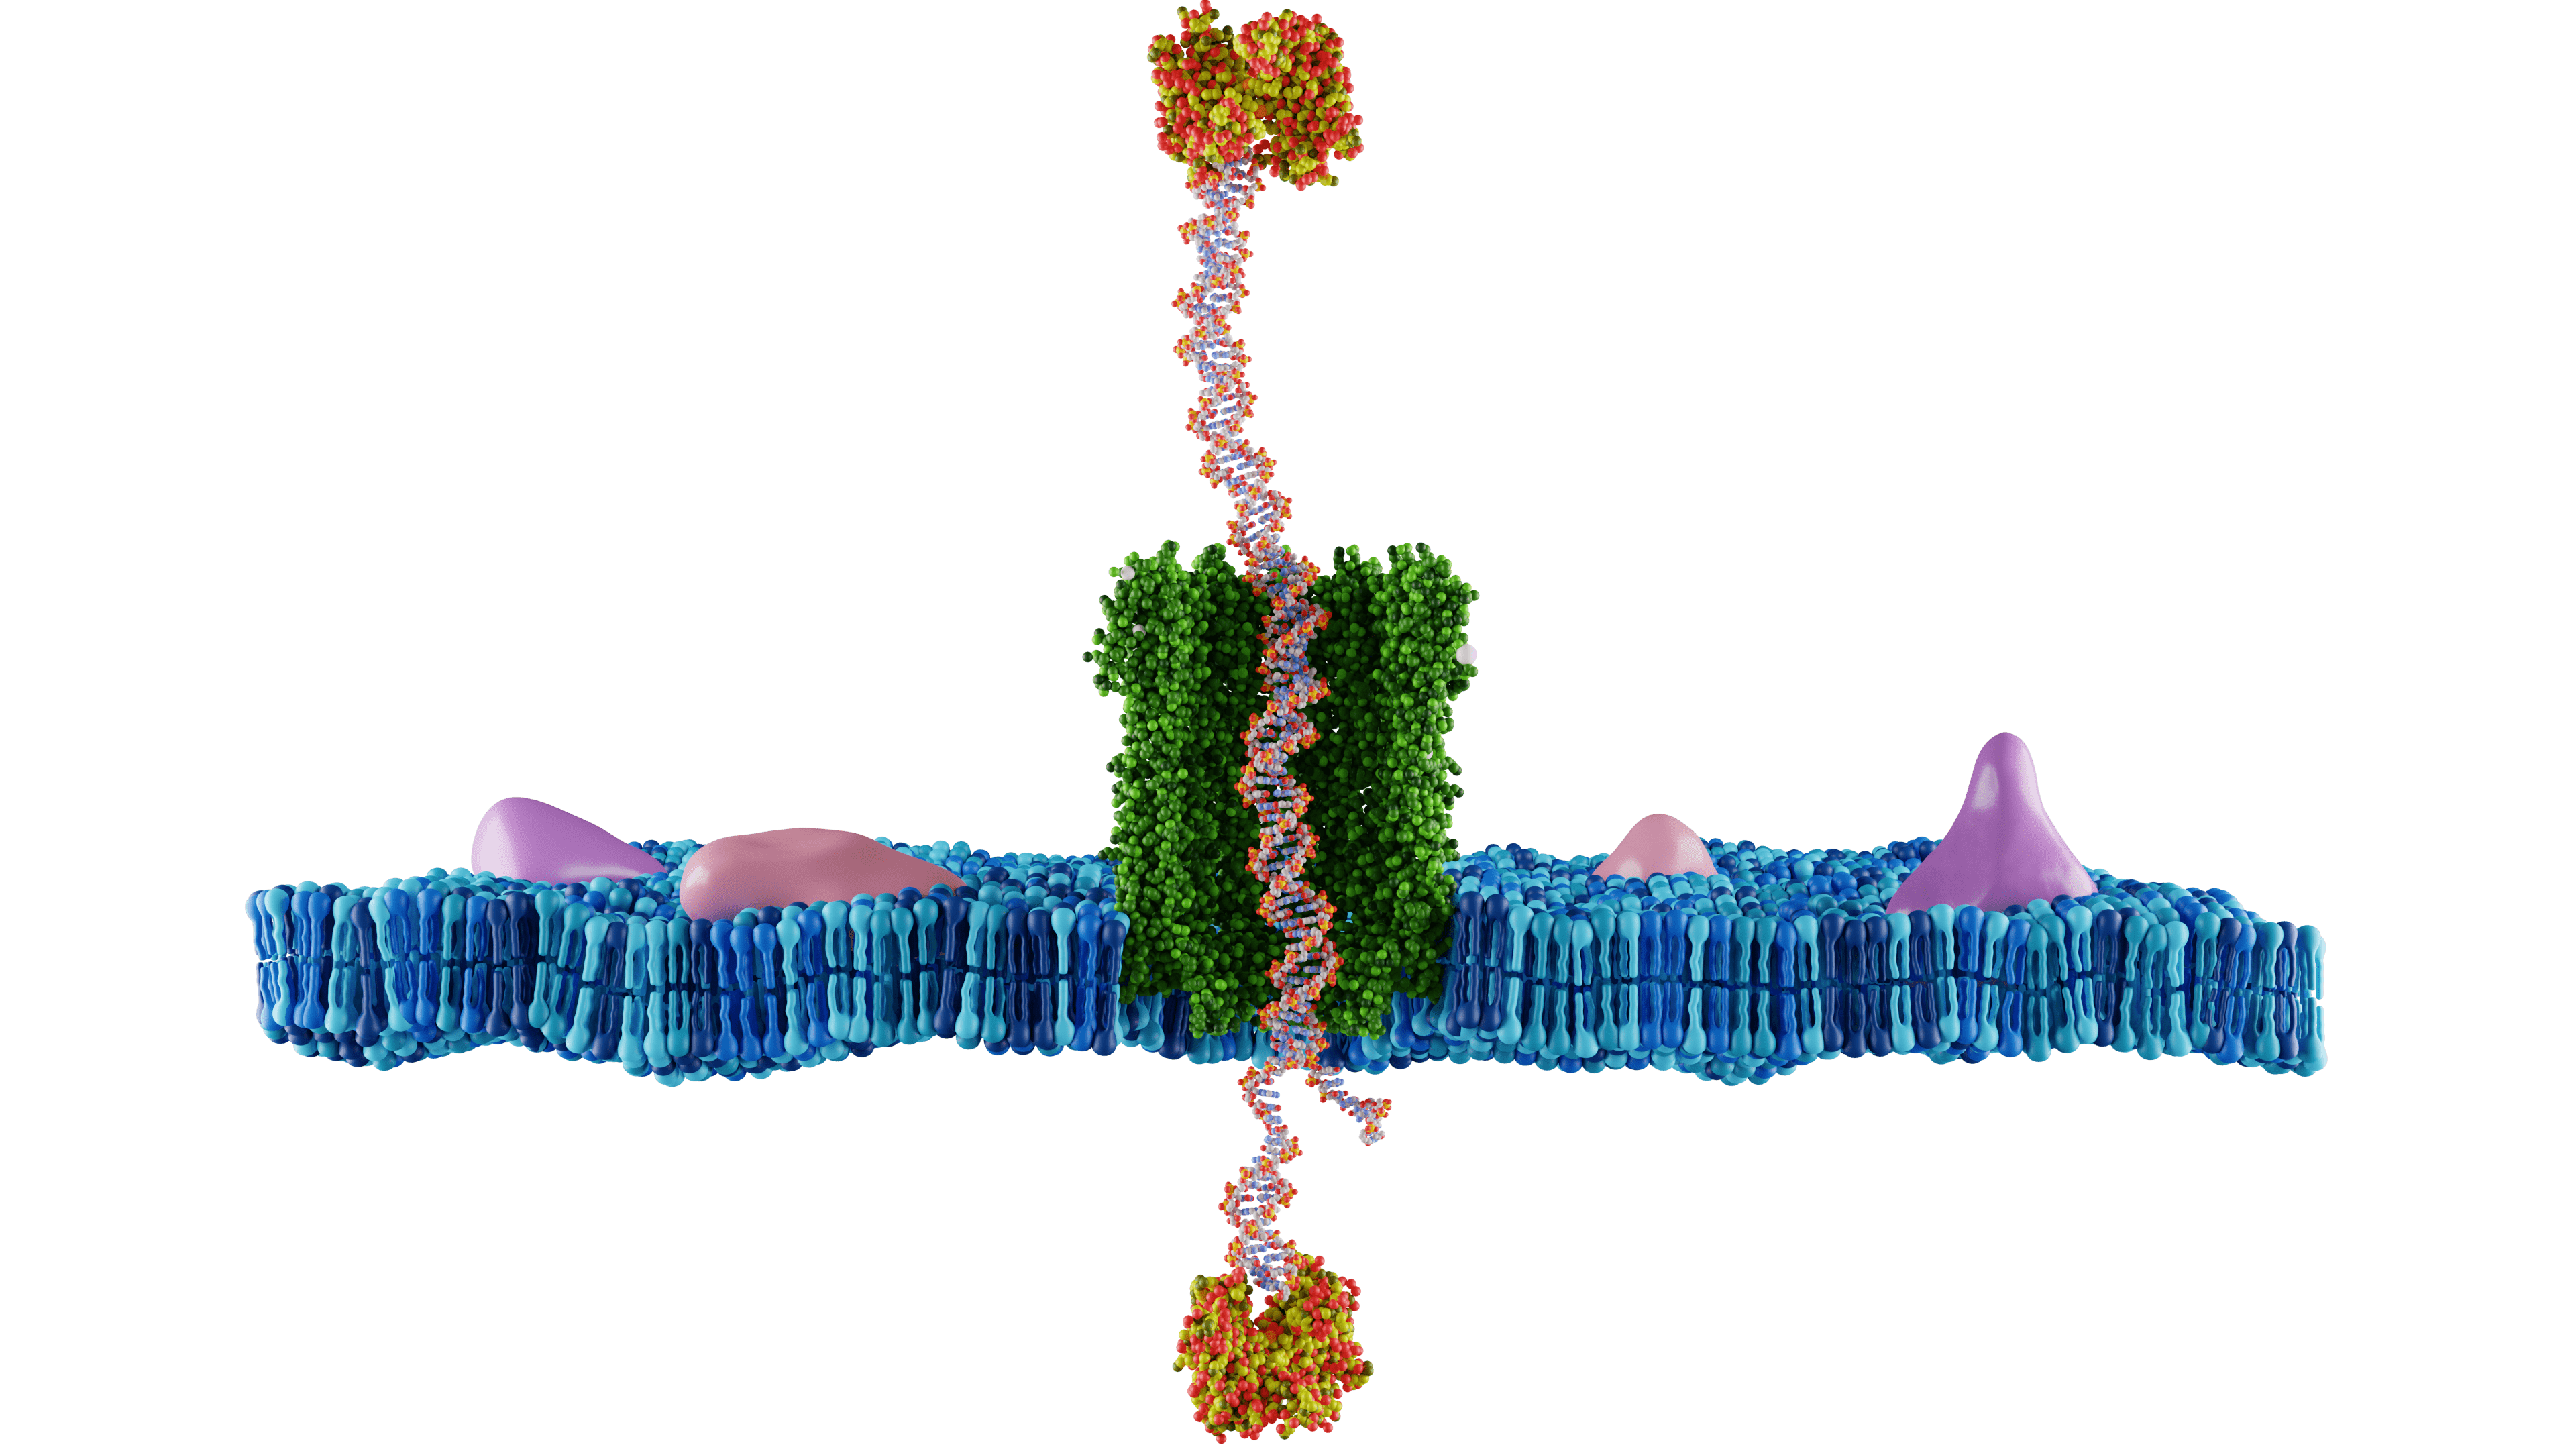
\includegraphics[height=9.5cm, width = 15.5cm]{Figures/CoverPhoto.png}
\vspace*{5.7cm}
\begin{center}
\begin{figure}[H]
\centering
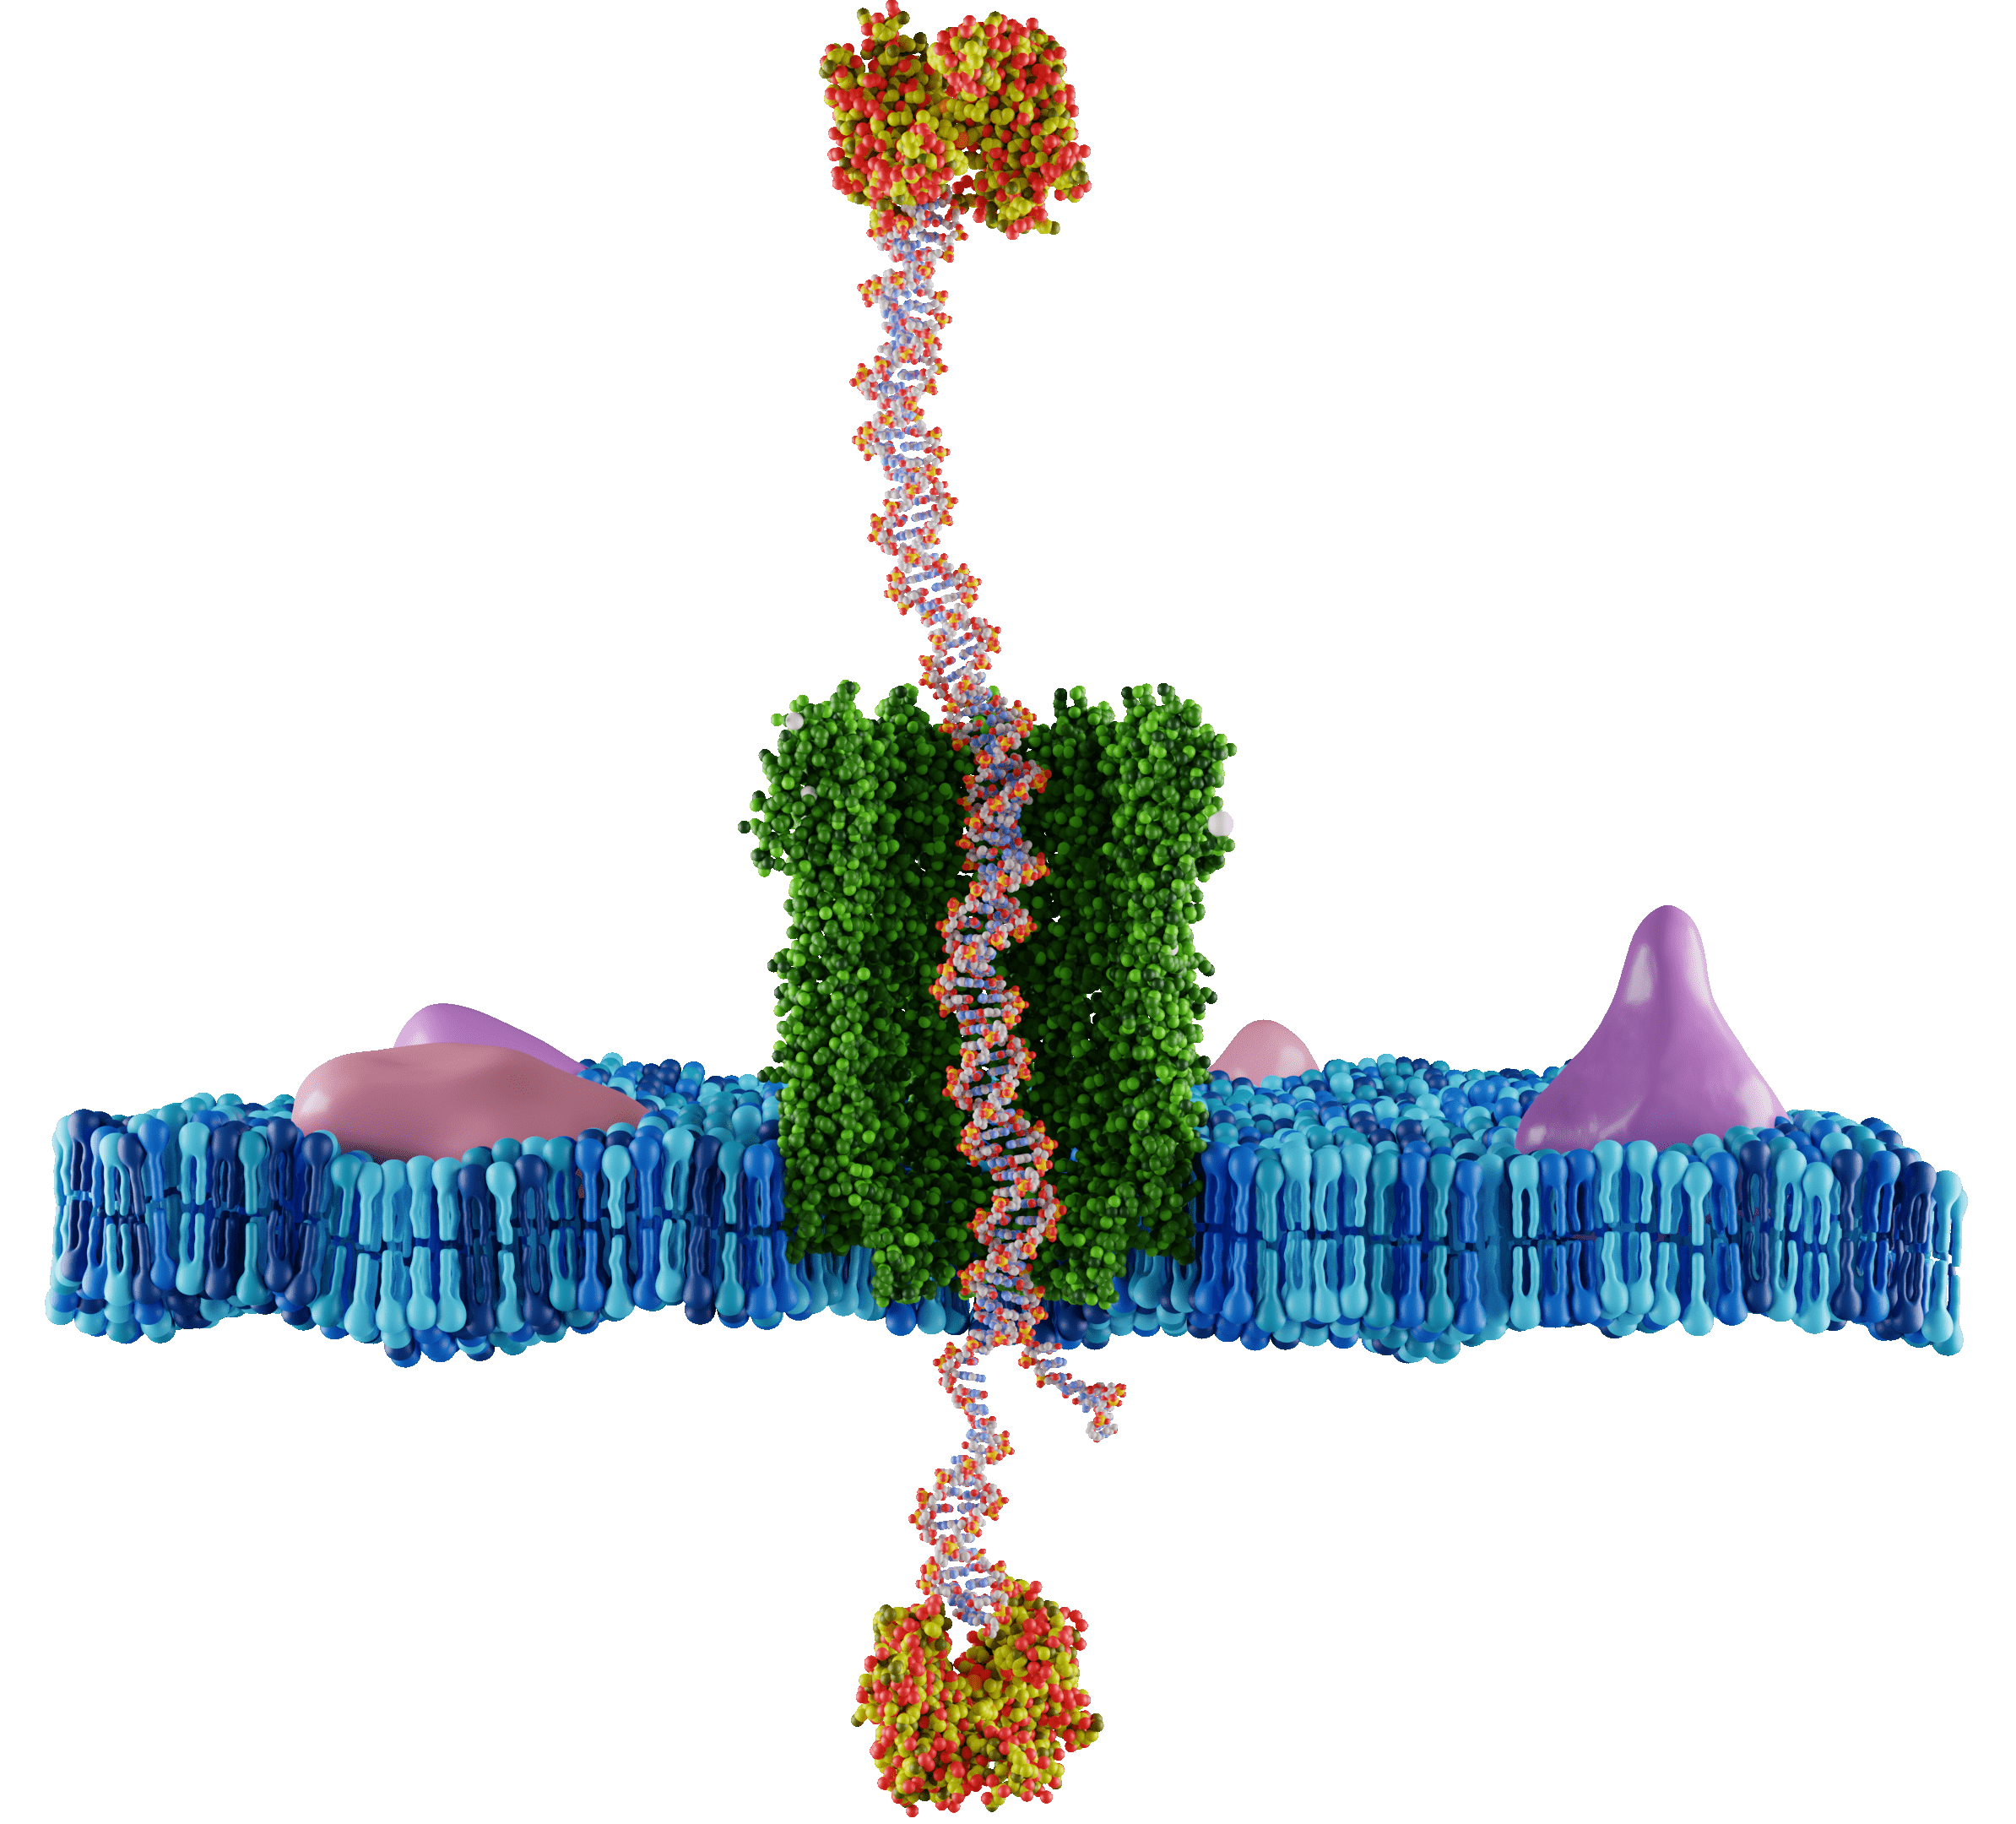
\includegraphics[scale=0.166]{Figures/CoverPhoto2.png}
\end{figure}
\end{center}
%
\vfill
 \cleardoublepage
\thispagestyle{empty}
\setlength{\parindent}{0cm}
\vspace*{\fill}

\begin{smallfont}
\copyright\ Copyright by KU Leuven \par
Without written permission of the promoters and the authors it is forbidden to reproduce or adapt in any form or by any means any part of this publication. Requests for obtaining the right to reproduce or utilize parts of this publication should be addressed to KU Leuven, Faculteit Wetenschappen, Geel Huis, Kasteelpark Arenberg 11 bus 2100, 3001 Leuven (Heverlee), Telephone +32 16 32 14 01.
A written permission of the promoter is also required to use the methods, products, schematics and programs described in this work for industrial or commercial use, and for submitting this publication in scientific contests.
\end{smallfont}

\setlength{\parindent}{0.5cm}
 \cleardoublepage
\setcounter{page}{0}
\pagenumbering{roman}

\addcontentsline{toc}{chapter}{Abstract}
\chapter*{Abstract}

Autonomous molecular machines are ubiquitous in the machinery of life, collectively
driving the molecular processes in our cells. Inspired by these biological machines,
scientists
develop synthetic devices performing specialised operations at the nanoscale. In this
thesis we study a specific molecular machine designed by Bayoumi et al.\cite{Bayoumi21},
which is composed of a DNA-neutravidin piston trapped inside a ClyA nanopore.

Using the free energy of DNA hybridisation this molecular machine is able to perform
autonomous and active transport of DNA cargo both following or opposing an
external bias force. During each operating cycle of the nanopiston a DNA cargo
is transported from the cis- to the trans-side of the membrane, in which the piston is
embedded.

Due to the length scale associated with molecular machines performing in depth
experimental studies has been proven to be challenging. During this thesis we aim
to shed light on the operating principles of the nanopiston by using molecular dynamics
simulations. Motivated by the computational cost of classical all-atom simulations a
coarse-grained model of the DNA nanopiston is designed.

Entropic interactions between the DNA piston and the nanopore are thought to
play an important role in facilitating the DNA transport. Studying these effects reveal
two distinct origins of entropic forces. Large double stranded DNA is kept predominantly
outside of the pore's constriction, by the entropic penalty of confinement.  Whereas, the
flexible single stranded DNA also
endouvours to maximize its available configurational space by opposing confinement.

Consecutively the  conformational fluctuations of
the nanopiston are studied.  These simulations clearly show the importance of the
entropic interactions promoting the operation cycle.  The entropic
penalty of confining the flexible single stranded DNA components of the piston in the
nanopore enable the continuation of the hybridisation reactions.

In an attempt to study a full piston cycle, the hybridisation reactions driving the
operation are simulated using our coarse-grained
model. Due to the inherent difficulty of simulating these reactions an advanced
sampling method called forward flux sampling is needed.
While performing these simulations the main limitation of our coarse-grained model is
encountered. The compliance of the biological nanopore is found to be essential in
facilitating the hybridisation pathways, but is not yet incorporated in our current
model.

\cleardoublepage
\cleardoublepage
\addcontentsline{toc}{chapter}{Samenvatting}
\chapter*{Samenvatting}
Summary in dutch.

\cleardoublepage
\addcontentsline{toc}{chapter}{Summary}
\chapter*{Summary}
Summary in english.
 \cleardoublepage
\printglossaries \cleardoublepage
%\addcontentsline{toc}{chapter}{List of Figures}
\listoffigures \cleardoublepage
%\addcontentsline{toc}{chapter}{List of Tables}
\listoftables \cleardoublepage
%\addcontentsline{toc}{chapter}{Contents}
\linespread{0.816}
{\small \tableofcontents}
\cleardoublepage
\linespread{1}

% MAIN MATTER
\mainmatter
\setcounter{page}{0}
\pagenumbering{arabic}

%% Introduction
\chapter{Introduction}
\vspace{-1cm}
\epigraphfontsize{\small\itshape}
\epigraph{“...if we were to name the most powerful assumption of all, which leads one on
and on in an attempt to understand life, it is that all things are made of atoms, and
that everything that living things do can be understood in terms of the jigglings and
wigglings of atoms.”}
{--- \textup{Richard P. Feynman}, The Feynman Lectures on Physics\cite{feynmanLectures}}
\section{Thesis outline}

All organisms in nature tirelessly perform work to keep their cellular functions
intact, opposing the ever increasing entropy in their environment. This work is
collectively performed by countless molecular machines, all contributing to
their specific tasks.

Despite being so abundantly present in nature, fabricating synthetic molecular machines
turns out to be a difficult task. One of the biggest hurdles in this process arises from
their corresponding length-scale. Often times these machines are not larger then
a few nanometres, making the typical energy associated with the bonds and
distortions of their structure comparable to thermal energy fluctuations. As a result of
these thermal fluctuations in their environment molecular machines naturally perform
a stochastic motion that complicates their functioning.  Extracting useful work from
these freely tumbling structures is almost impossible. To overcome this limitation most
synthetic molecular machines are embedded in a larger complex providing necessary
stability.\cite{Watson2016}

This phenomenon is also observed in nature, for instance in the interfacing of protein
complexes with the phospholipid bilayer of cells.  A wildly known example is the
bacterial flagellar motor, shown in Figure \ref{fig:flagella}. The function of this
machine is providing an efficient way for bacteria to
roll and tumble throughout their environment. Just like in electrical motors, the
flagellar motor consists of a stator and a rotor. The stator is anchored into the cell
membrane,
while the rotor is allowed to freely rotate. The work is produced by the flow of cations
through the stator. Inducing changes in the electrostatic interactions between the two
parts of the flagellar motor generates a unidirectional motion.\cite{sowa_berry_2008}

Similarly to macroscopic engines, heat is produced during the operation of molecular
machines. When the structure is not capable of dissipating this heat efficiently, an
excessive build-up compromises its durability. To mitigate this problem, large and soft
molecules are often used in the design of nanomachines. A logical choice
is the use of polymers, which can effectively dissipate heat as a result of their
flexibility.  Due to the programmability of DNA, using the Watson-Crick interactions,
the DNA polymer provides additional aptitude. This makes DNA a popular material in
nanotechnology.

The central topic of this thesis is studying a synthetic molecular machine consisting of
a DNA nanopiston embedded into a phospholipid membrane, as depicted on the cover page.
The structure was designed by Bayoumi et al. with the aim of performing
selective transport of DNA through a membrane.\cite{Bayoumi21} This
nanopiston can be characterised as an autonomous molecular machine, which turns over
chemical fuel to continuously perform work.

% The operation cycle of previously designed DNA transporters requires a supporting
% external bias.\cite{Franceschini2013} However, this specific nanopiston also operates
% opposing an external bias force. The physics driving this machine is entropy and will be
% discussed in detail in throughout this thesis.

In the first chapter a comprehensive introduction of important concepts
regarding the DNA nanopiston is given. Having laid this theoretical foundation, the
structure and operation cycle of the DNA nanopiston is discussed in chapter two. Next the
computational model used in this thesis is presented in chapter three. In chapter four,
the results of these simulations is discussed. Finally chapter five will offer a
discussion of these results and recommendations for further research.
\vspace{0.5cm}
\begin{figure}[ht!]
\begin{center}
  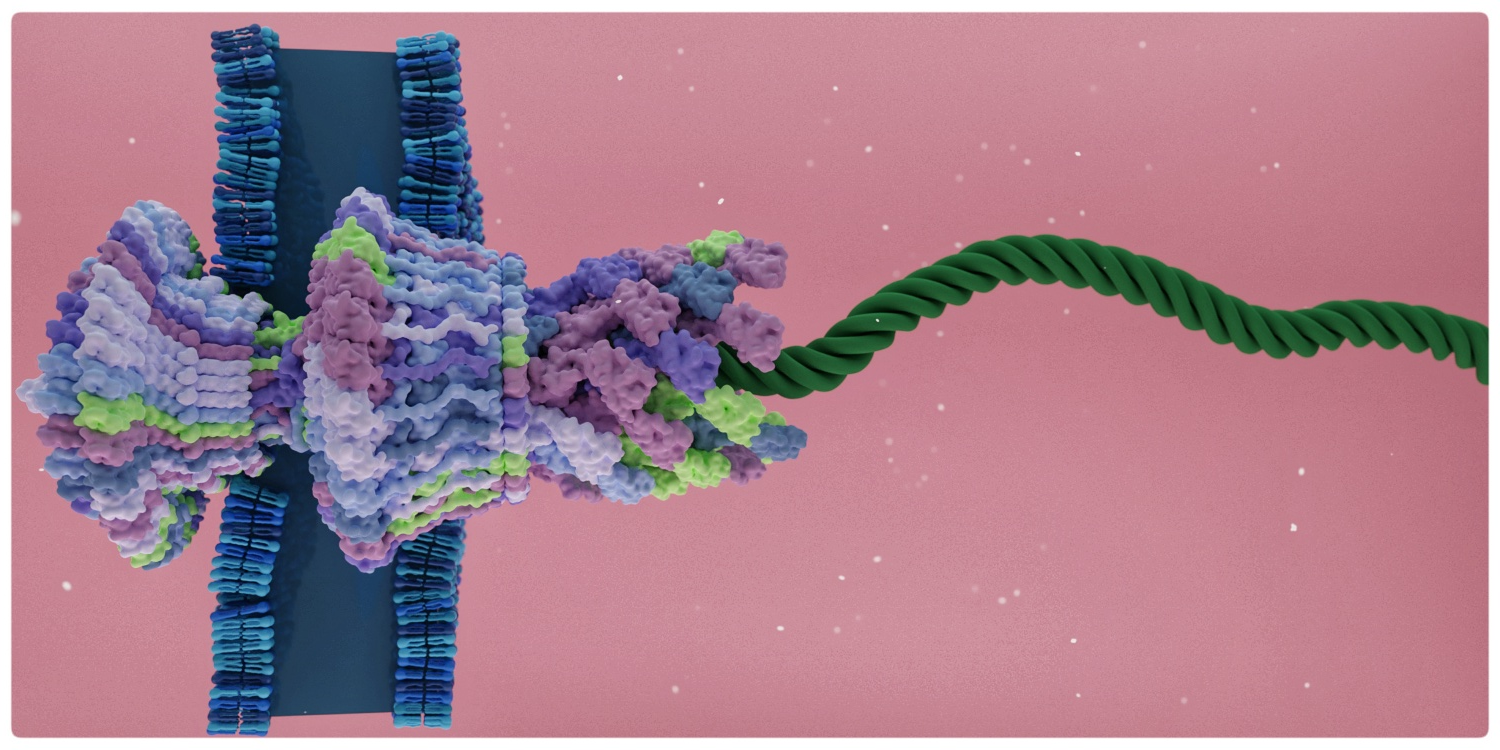
\includegraphics[width=0.85\textwidth]{Figures/flagella2.png}
  \caption[Render of a flagellar motor-hook complex, based on the cryo-EM structure of
  the Salmonella flagellar motor.] {Render of a flagellar motor-hook complex embedded in
  a
  cell membrane. The merged density map of the flagellar motor was obtained from the
  cryo-EM structure of the Salmonella flagellar motor and
  prepared using
  ChimeraX.  Both the cell membrane and the flagella are interprations. Image was
rendered using Blender.\cite{Tan2021, blender,
ChimeraX}}
  \label{fig:flagella}
\end{center}
\end{figure}


\section{Biological Nanopores}

Biological nanopores are small perforations in a lipid bilayer, created
by a pore forming protein.  The majority of these proteins are toxins produced by
pathogenic bacteria, as means of killing targeted cells. They work by perforating the
membrane of a cell, causing cell depolarization and inducing an osmotic potential.
These effects disrupt vital cell functions or spill its nutrients into the
environment, often times resulting in the killing of the cell.\\

The reason scientists are interested in studying nanopores is related to their size.
These protein structures are generally only a few nanometres in diameter, making them
comparable in size to the tiny transistors found in modern computers.
Working at these small scales has the unavoidable complication, that it becomes difficult
to retrieve information from nano scale processes.
Developing sensors to probe this exotic length scale is thereby very relevant. This is
the exact problem nanopores provide a solution to, i.e. spectroscopy at the smallest
scale.\\

Before delving into ionic current spectroscopy, the primary application of these
nanopores, first a brief overview will be given of the structural properties of two
popular biological nanopores.

\subsection{$\alpha$-Hemolysin ($\alpha$-HL)}

The $\alpha$-Hemolysin ($\alpha$-HL) protein is the most commonly used pore forming
proteins to create biological nanopores. It is produced by the Staphylococcus aureus, a
bacterium commonly found in human microbiota.\\

The $\alpha$-HL pore(PDBID:...) is an oligomeric complex with multiple naturally
occurring variations. The most typical configuration
is a heptameric structure, meaning that there are seven protomers found in the complex.
The secondary structure elements consist principally of $\beta$-sheets, making it a
member
of the $\beta$-barrel pore-forming toxins. Through both electrostatic and hydrophobic
interactions, the $\alpha$-HL is bound to the membrane of a target cell. Here the
monomers assemble to a 'prepore' complex that transitions to the stable pore complex by
inserting the $\beta$-barrel into the membrane.\\

Structurally the shape of $\alpha$-HL resembles that of a hollow mushroom. The total
hight of the complex is 11nm and the maximum width is measured to be 10nm. The internal
chamber of the pore located at the cis side of the membrane is called the lumen.
The lumen of $\alpha$-HL is quite constricted measuring a diameter of 3nm. At the
membrane, the lumen chamber transitions into a protein stem, referred to as the
constriction of the pore further reducing the diameter of the chamber to a minimum of
1.5nm. Over the inside surface of  $\alpha$-HL the charges are relatively uniformly
distributed, which will play an important role in further applications.\\

\begin{figure}[h!]
  \centering
  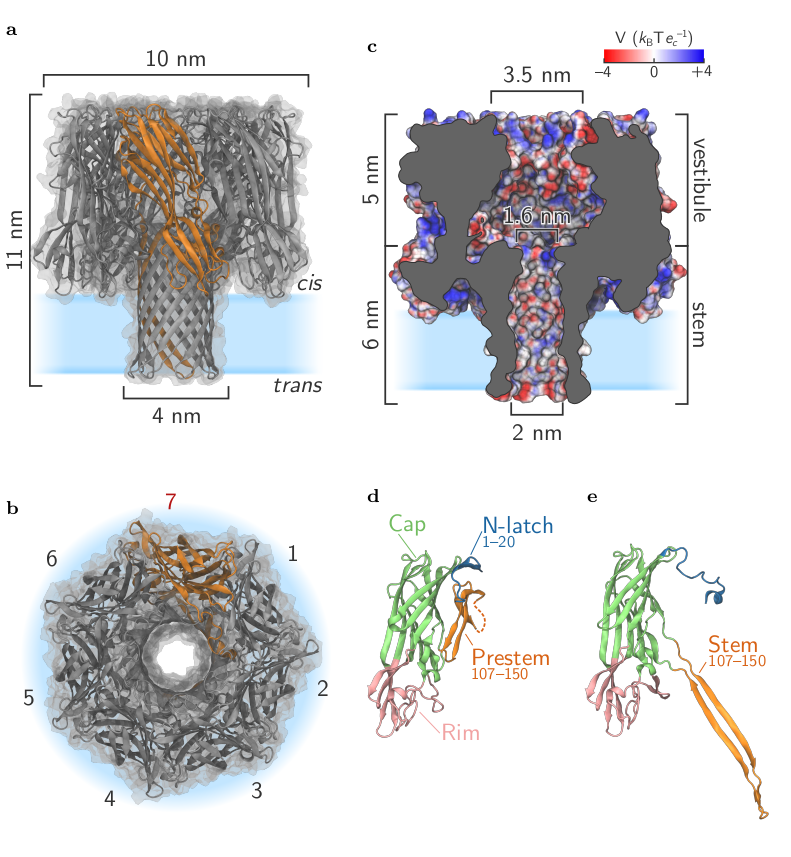
\includegraphics[width=0.5\linewidth]{Figures/alpha-hemolysin.png}
  \caption{write caption}
  \label{adsf}
\end{figure}


\subsection{Cytolysin A (ClyA)}

The Cytolysin A (ClyA) is a larger type of pore forming protein, first found to be
secreted by E. coli strains. The larger size of its lumen allows for different types of
applications, compared to smaller complexes like $\alpha$-HL. Most relevant for this
thesis, is the fact that the larger diameter of the pore's stem allows for translocation
of double stranded DNA.\\

The ClyA pore (PDBID:6MRT[cite]) is an oligomeric complex most typically found in a
 dodecameric configuration is, meaning that there are twelve protomers found in the
complex. In nature there are found small variations on this configuration. The secondary
structure elements consist principally of $\alpha$-helices, making it a member of the $
\alpha$-pore-forming toxins. The protein formation is induced by the hydrophobic
interactions between the $\beta$-hairpin and the solvent. The main structural
rearrangement in this process consists of swinging
out this $\beta$-tongue and inserting it into the membrane. After this transition, the
membrane-bounded monomers oligomerize to from the final pore structure.

Structurally the shape of ClyA resembles that of two hollow cylinders stacked on top of
each other. This cylinder approximation will be important later on in this thesis, where
it will be used to create a simplified model of the nanopore. The total hight of the
complex is
14nm and the maximum width is measured to be 11nm. The lumen's size of this nanopore
differentiates it from the previously discussed $\alpha$-HL. The cis entrance of the
lumen measures 6nm, while the constricted side of the pore is still 3.6nm in diameter. In
contrary to the $\alpha$-HL, the inside surface of ClyA has a net negative charge,
making it cation sensitive. This excess charge will induce an important
 coulomb interaction between the pore and negatively charged analytes.


\begin{figure}[h!]
  \centering
  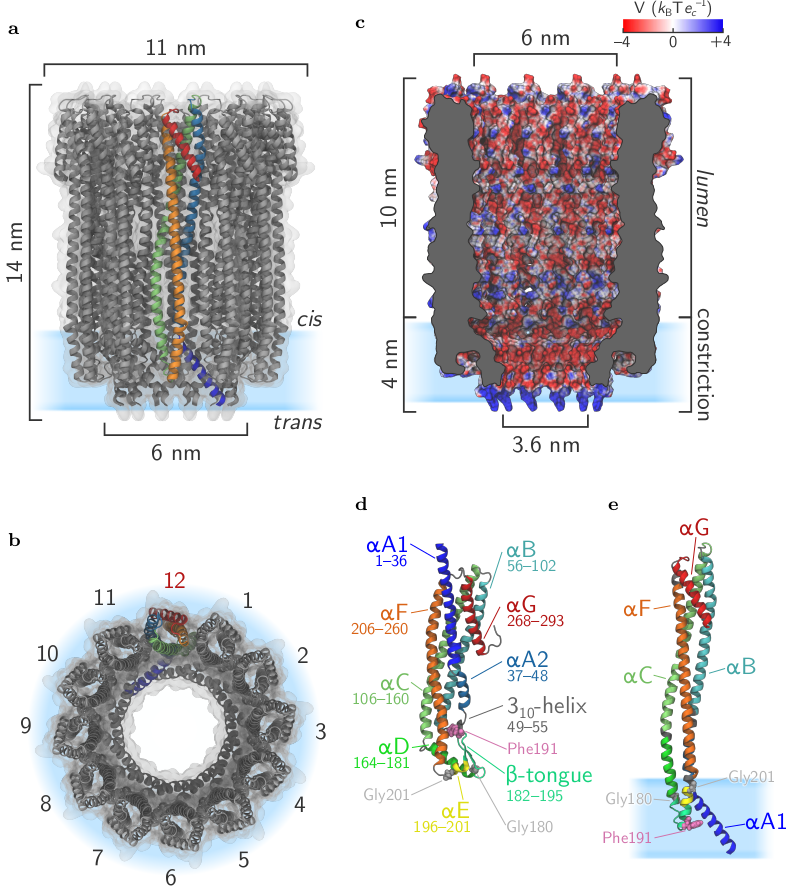
\includegraphics[width=0.5\linewidth]{Figures/cytolysinA.png}
  \caption{write caption}
  \label{adassf}
\end{figure}

\subsection{Ionic current spectroscopy}
In recent years the study of nanopores became a popular research domain, mainly
due to the development of the nanopore-based ionic current spectroscopy. For the case of
biological nanopores, this method depicted in figure ... A lipid bilayer is perforated
using a pore forming protein, for example $\alpha$-HL. The membrane separates two
chambers of a basin filled with a saline solution. When a potential difference is created
over the membrane, the nanopore mediates an ion current between the two sides of the
basin.

This ion current through the pore can accurately be measured. If the pore is empty we
refer to the measured current as the open pore current.  However the applied electric
field also induces forces upon analytes dissolved in the basin. The net result of these
interactions is a flux of analytes towards and in some cases through the nanopore.
Analytes located inside of the nanopore partially block the ion current through the pore,
reducing the measured current. Using machine learning algorithms, the time series of
these current fluctuation can be measured and identified with particular analytes in the
basin. These methods are so precise, that they allow for single cell spectroscopy.

It should be noted that besides these biological nanopores, there are also inorganic
nanopores under development. An example of inorganic nanopres are solid state nanopores,
created by making perforations in a semi-conductor wafer. While currently not as
accessible as biological nanopres, mainly due to their high production cost, this method
has some major advantages. First of all the material properties provide a chemical
robustness not
present in biological nanopores. The production process also allows for easy scalability
and customisability. While currently not as widely used as biological nanopores, due
to their customisability and robustness, solid state nanopores will prove to be an
important asset in future nanotechnology.

\section{Deoxyribonucleic acid (DNA)}

\begin{wrapfigure}{r}{0.23\textwidth}
  \begin{center}
    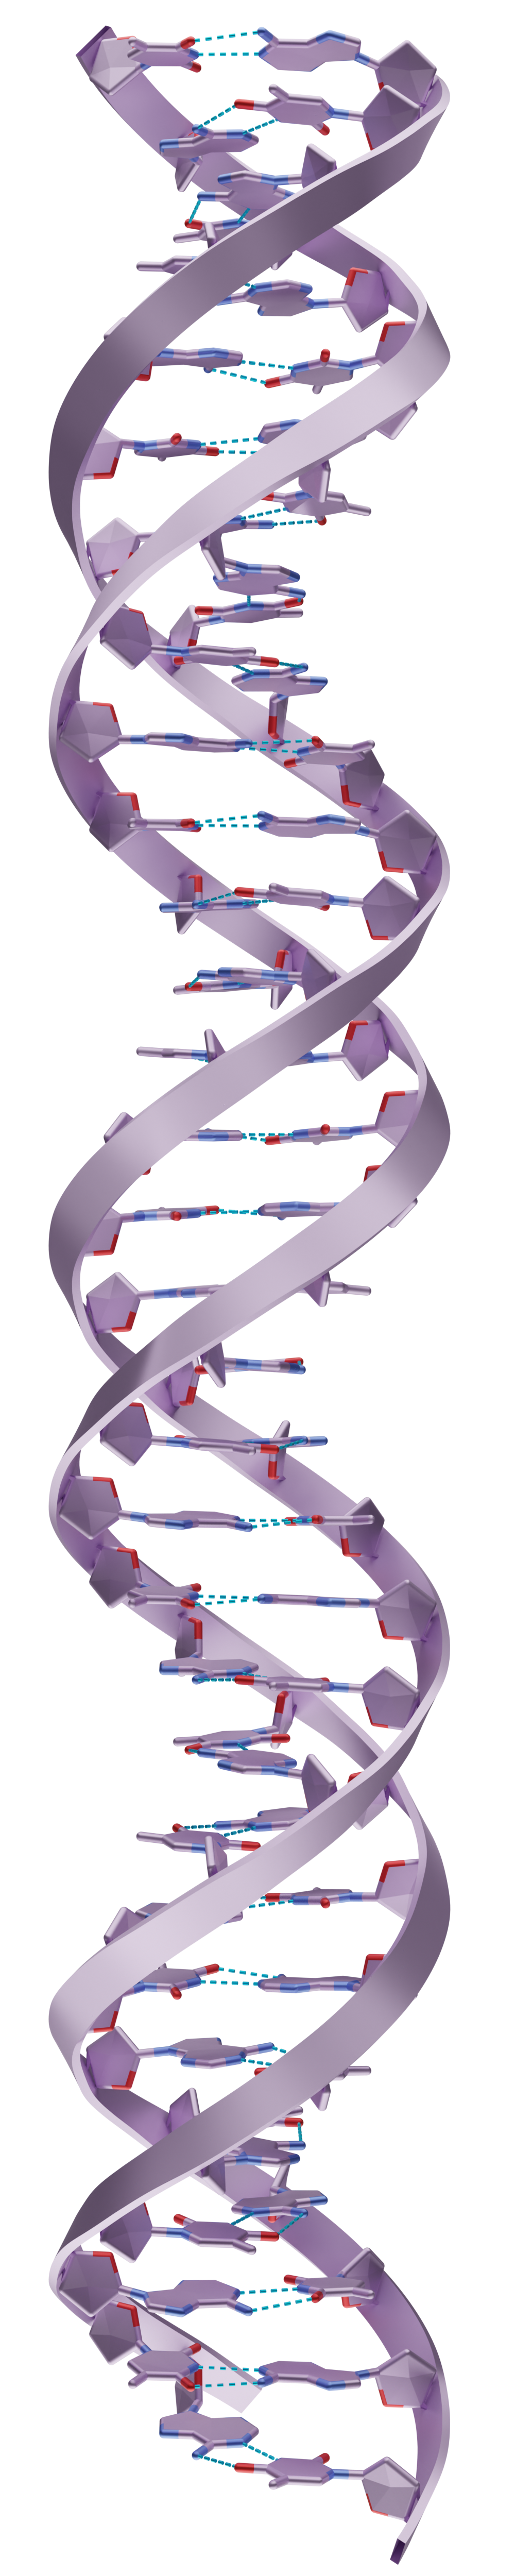
\includegraphics[width=0.20\textwidth]{Figures/cartoon2.png}
  \end{center}
  \caption{caption nog maken}
\end{wrapfigure}

Deoxyribonucleic acid (DNA) is a long biopolymer composed of two strands, commonly found
in its characteristic double helix structure. DNA is most famously know for storing the
genetic code of organisms in the nucleus of their cells. The existence of this genetic
code was already
postulated by the Greek philosopher Aristotle. He developed a heredity theory, based
upon "blueprints", in which he tried to explain why physical traits where passed on from
generation to generation. This theory would go unnoticed until in 1869
Friedrich Meicher discovered a new microscopic substance found on discarded
surgical bandages. He would call this substance "Nuclein" since it originated
form the nucleus of the cell. Later it was found that this new substance, currently known
as "Deoxyribonucleic acid" or DNA, plays an important role as a blueprint for the
perpatuation of living matter.

The structure of DNA was first determined by Rosalind Franklin using X-ray
crystallography. Later this research was published by Watson and Crick [.], who concluded
that DNA consists of two individual strands, coiled around each other in a double helical
structure. Each strand is a chain of monomers, which we call nucleotides. A nucleotide is
made up of a
deoxyribose sugar, phosphate group and one of four nitrogenous bases: cytosine(C),
guanine(G), adenine(A) or thymine(T). The covalent bonds that give both strands structure
are formed between consecutive phosphate groups, which together make up the DNA backbone.
To form the double helix, two backbones are held together by
selective hydrogen bonds occurring between corresponding bases of opposing strands. These
dipole interactions give rise to a selection rule, forming only A-T and C-G base pairs.

Since the binding of the two strands is mediated by hydrogen bonding, association and
dissociation is possible. The study of these processes is called DNA thermodynamics. The
dissociation process of double stranded DNA (dsDNA) is called DNA melting, resulting in
two individual strands of single stranded DNA (ssDNA). The reverse process is called DNA
hybridisation, which is the selective binding of complementary nucleotides to form dsDNA.

The double helix structure of DNA comes in three different types, B-DNA, A-DNA and Z-DNA,
all having a slightly different geometric arrangement. In nature the B-form is most
commonly observed, which is characterised by a right-handed helix and the coplanarity
between the complementary bases as shown in Fig. ... . A helical twist of B-DNA consists
of around 10 base pairs, having a net helical pitch of $0.34 nm$. During this thesis,
when analysing DNA we refer to the B-DNA form.

When studying DNA the statistical theory of polymer physics is a useful tool. An
atomistic resolution is not always needed to accurately describe processes involving
relatively long DNA strands.  Reducing the complexity of DNA to the monomer level is
often justified, allowing us to use more general results in polymer physics.



\section{Polymer Physics}
A polymer is a biomolecule made up of building blocks called monomers, linked together to
from a chain. The configuration of this chain is determined by the position vector of
each monomer, denoted as $\{\boldsymbol{r}_0, \boldsymbol{r}_1, \dots,
\boldsymbol{r}_N\}$.  The link between each consecutive pair of monomers is called the
bond-vector, defined as
$\boldsymbol{u}_i = \boldsymbol{r}_i - \boldsymbol{r}_{i-1}$. During this discussion we
will assume these bonds to be inextensible, i.e. having a fixed
bond length of $|\boldsymbol{u}_i| = a$.\\


Various different models can be used to describe a polymer. The most simple version is
called
the Freely Jointed Chain (FJC). This model is an example of an ideal flexible polymer, in
which excluded volume interactions or polymer bending rigidity are not taken into
account.  In this
model, it is assumed that each bond-vector is completely uncorrelated with its adjacent
bonds. Mathematically this is represented by assigning the bond-vector orientation
an uniform probability distribution
\begin{equation}
    g(\boldsymbol{u}) = \frac{1}{4 \pi a}
    \delta(|\boldsymbol{u}| - a), \\
\end{equation}
where $a$ is the fixed bond length.


The above described model provides a relatively accurate description of long polymers.
However, the assumption that consecutive monomers are uncorrelated becomes
problematic at small length scales. The Kratky-Porod model, or discrete wormlike chain,
solves this problem by taking the energetic cost of bending the polymer into
account. Mathematically this is done introducing a bending rigidity between neighbouring
bonds in the form of a coupling constant, $\kappa >0$. Each polymer configuration is
assigned an energy using the equation,
\begin{equation}
    E_{WLC}= -\kappa \sum_{i=1}^{N} \boldsymbol{\hat{u}_i} \cdot
    \boldsymbol{\hat{u}}_{i+1}
    = -\kappa
    \sum_{i=1}^{N} \cos\theta_i,
    \label{wlc}
\end{equation}
where $\boldsymbol{\hat{u}} = \boldsymbol{u}/a$ is the unit bond-vector and $\theta_i$ is
the angle between neighbouring bond-vectors $\boldsymbol{\hat{u}_i}$ and
$\boldsymbol{\hat{u}_{i+1}}$. The lowest energy state of this discrete wormlike chain is
a straight rodlike configuration, where the bond angles $\theta_i$ are minimized.

To calculate the bond-vector correlation function,  we first determine the partition
function, $Z_{WLC}$, of the system. Identifying the single monomer contributions, this
quantity factorises into a product of single bond-vector partition functions as
\begin{equation}
    \begin{aligned}
        \label{210}
        Z_{\mathrm{WLC}}(N, T)
        &= \int_{0}^{\pi}\dots \int_{0}^{\pi} d \theta_1 \dots d \theta_N \sin \theta_1 \dots
        \sin \theta_N\ e^{\beta \kappa \sum_{i=1}^{N-1} \cos\theta_i}\\
        &= \left[\int_{0}^{\pi} d \theta \sin \theta e^{\beta \kappa \cos
        \theta}\right]^{N}\\
        &= \left[Z_{\mathrm{WLC}}(1, T)\right]^{N},
    \end{aligned}
\end{equation}
where $\beta=1/\kappa_b T$ is the inverse temperature. It rests us to determine the
single bond-vector partition function. Carrying out the integration yields the result,
\begin{equation}
    Z_{\mathrm{WLC}}(1, T)=\int_{0}^{\pi} d \theta e^{\beta \kappa \theta}=\frac{2
    \sinh(\beta \kappa)}{\beta \kappa}.
\end{equation}

%\begin{equation}
%    \left\langle\cos \theta_{i+1}\right\rangle
%    =\frac{\partial \log Z_{\mathrm{WLC}}(1, T)}{\beta \partial \kappa}.
%\end{equation}

From the found partition function we can now determine the bond-vector correlation
function. Using the definition of the partition function, we determine the average cosine
of the angle between consecutive bonds to be,
\begin{equation}
    \begin{aligned}
    \left\langle\cos \theta_{i+1}\right\rangle
    &=\frac{\partial \log Z_{\mathrm{WLC}}(1, T)}{\partial(\beta \kappa)}\\
    &= \frac{1}{\tanh(\beta \kappa)} - \frac{1}{\beta \kappa}.
    \end{aligned}
\end{equation}

Studying the conformation of polymers is often times done assuming a low
temperature or large bending rigidity, where we find
that the above expression simplifies. In the limit, $\beta \kappa \gg 1$, the lowest
order approximation yields,
\begin{equation}
    \langle\cos \theta\rangle \approx 1-\frac{1}{\beta \kappa}.
\end{equation}

Decomposing the bond-vector $\boldsymbol{\hat{u}}_{n+1}$ in terms of an orthonormal
basis, defined by the normal and tangential directions of the preceding vector
$\boldsymbol{\hat{u}}_{n+1}$, gives
\begin{equation}
\boldsymbol{\hat{u}}_{n+1} = \boldsymbol{\hat{u}}_{n} \cos \theta_{n} +
\boldsymbol{\hat{u}}_{n}^{\perp} \sin \theta_{n}.
\end{equation}
This decomposition allows us to express the correlation between distant bond-vectors in
terms of the correlation between neighbouring bonds-vectors. The factorisation
yields
\begin{equation}
\begin{aligned}
    \left\langle\boldsymbol{\hat{u}}_{i} \cdot \boldsymbol{\hat{u}}_{i+m}\right\rangle
    &=\left\langle\boldsymbol{\hat{u}}_{i} \cdot
        \boldsymbol{\hat{u}}_{i+m-1}\right\rangle\left\langle\cos
    \theta\right\rangle = \dots =\langle\cos \theta\rangle^{m},
    % &=\exp \bigg{[} -\frac{n a}{l_{b}} \bigg{]},
\end{aligned}
\end{equation}
where we used the fact that the sinusoidal terms vanish due to symmetry.
Exploring this result in the limit, $\beta \kappa \gg 1$, we find the expression
\begin{equation}
    \left\langle\boldsymbol{\hat{u}}_{i} \cdot \boldsymbol{\hat{u}}_{i+m}\right\rangle =
    e^{m \log(1 - \frac{1}{\beta \kappa})} \approx e^{-na/l_p},
\end{equation}
introducing a new polymer quantity, the bending persistence length

\begin{equation}
    l_b \equiv \frac{a \kappa}{k_{b} T}.
\end{equation}
This general result in polymer physics states that the correlations between bond-vectors
is exponentially decreasing. The defined quantity represents the characteristic
length scale of the polymer, over which the correlations between
bond-vectors is lost.

Two limiting cases can be explored. Firstly, in the
case where the persistence length is much larger then the polymer's length, $l_p \gg na$,
all bond-vectors are correlated, i.e. the polymer approximates a straight rod. For the
reverse case, where $l_p \ll na$, it can easily be shown that the polymer behaves as a
stochastic walk.

The persistence length is a central result in the theory of polymer physics, providing a
measurable quantity related to the bending rigidity of a polymer. During the
simulations performed in this thesis, the notion of bending persistence length is used to
discuss the flexibility of the DNA polymer.


%The end-to-end vector $\boldsymbol{R}$ in the continuum limit. For example can be
%rewritten using the arc-length parameter $s$ where $0 \leq s \leq L$ and $L = Na$ as:
%\begin{equation}
%    \label{hoi}
%    \langle\widehat{u}(q) \cdot \widehat{u}(q+s)\rangle= e^{-s / l_{\mathrm{p}}}.
%\end{equation}
%The continuum version of the end-to-end vector
%\begin{equation}
%    \boldsymbol{R}=\int_{0}^{L} \widehat{u}(s) d s.
%\end{equation}

%\begin{equation}
%\begin{aligned}
%    \left\langle\boldsymbol{R}^{2}\right\rangle
%    &= \int_{0}^{L} d s d s^{\prime}\left\langle\widehat{u}(s) \cdot
%  \widehat{t}\left(s^{\prime}\right)\right\rangle \\
%    &= 2 l_{\mathrm{b}} L\left\{1-\frac{l_{\mathrm{b}}}{L}\left(1-e^{-L /
%l_{\mathrm{b}}}\right)\right\}.
%\end{aligned}
%\end{equation}


\newpage
\section{Computer Simulations}

The theory of classical mechanics is often regarded as the first major breakthrough in
the field of physics. For every aspiring physicist this is still the starting point of
their studies. Unfortunately, getting to know these relatively simple laws of nature,
leads to the inescapable realisation that these theories are expressed in mathematical
formalisms that are only analytically solvable in few idealised scenarios. Applying these
formulas to a problem consisting of just more then two particles already leads to
practically unsolvable equations.\\

Although it is often times not possible to find an exact solution to equations
related to complex physical systems, finding reasonable approximations to their solution
is achievable. One popular method to analyse the dynamics of complex systems is the use
of simulations.\\

\begin{wrapfigure}{r}{0.5\textwidth}
  \begin{center}
    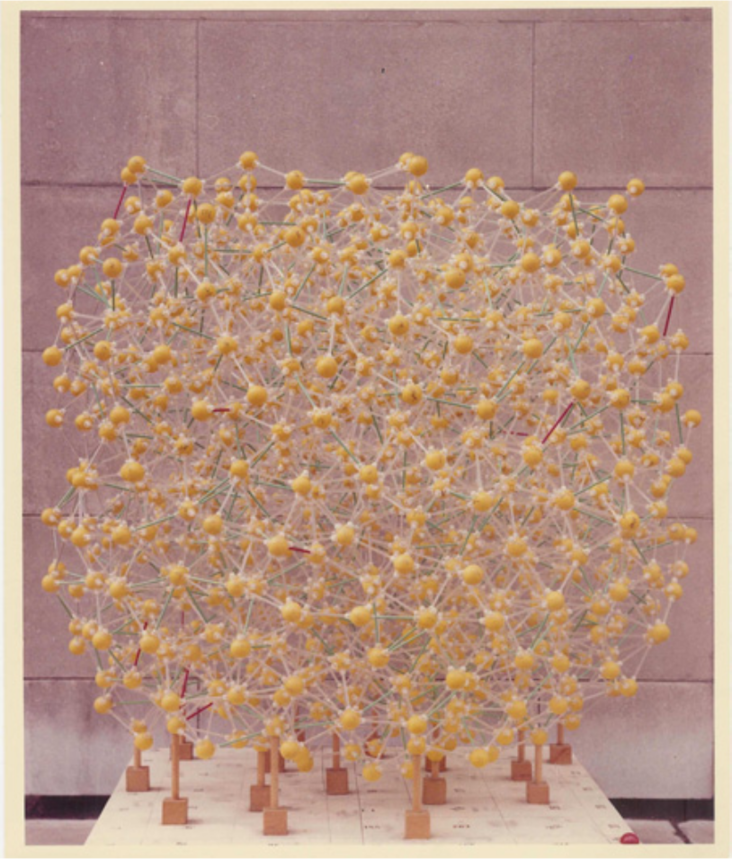
\includegraphics[width=0.38\textwidth]{Figures/WaterModel.png}
  \end{center}
  \caption{Example of an expanded model of a simple liquid (J L Finney, Ph.D thesis)}
\end{wrapfigure}

Simulations have a rich history within physics and engineering, starting even before the
invention of the computer.

\todo{dit weg laten??? misschien te veel bla bla}
An example of one of these mechanical simulations is the Waterloopkundig Laboratorium or
currently the waterloopbos, a scale model of important
Dutch waterways, where the influence of waves on harbours and docks was studied. This
simulation provided revolutionary insights into the behaviour of water and played an
important part in the design of the famous Delta Works.\\

Another more relevant example is the use of mechanical simulations to study the
structure of water.  In the early 20th century physicist J.D. Bernal and his fellow
researchers build various ball and stick models of water to analyse the possible 3D
configurations of water molecules in a liquid. Their research eventually explained the
peculiar physical properties of water from a atomistic perspective. However useful these
mechanical simulations turned out to be, the biggest drawback of the method was the
extreme cost of labour involved with their construct. As Bernal alluded to in his
famous 1962 lecture,

\begin{quote}
\dots I took a number of rubber balls and stuck them together with rods of a
selection of different lengths ranging from 2.75 to 4 inch. I tried to do this in the
first place as casually as possible, working in my own office being interrupted every
five minutes or so and not remembering what I had done before the interruption.\dots
\end{quote}

After the first computer simulations where performed in the Los Alamos labs, the
popularity of simulations rapidly increased. The remarkable explanatory power of
simulations, combined with the relative easy construction of computer models, lead to a
fast adoption of computer simulations in the scientific community. Within the context of
this thesis, computer simulations are used to study the mechanics of
the DNA polymer. Due to the high number of atoms in a typical system, it is generally
not possible to find an analytical solution to their equations of motion. In this
context, simulations are often used to gain an insight into the complex dynamics of the
system and guide the developments of more simple approximate theories. The simulations
act as a bridge between the microscopic constituents of the systems and the macroscopic
properties we want to understand.


\subsection{Molecular Dynamics Simulations}
Molecular Dynamics (MD) is a computer simulation technique, used to analyse
the dynamics of a classical many-body system. The central idea of this method is to
generate all the trajectories in a system of $N$ particles by numerically
integrating the classical equations of motion,
\[
m_i \frac{d^2 \boldsymbol{r_i}}{dt^2} = \boldsymbol{f_i}, \quad \boldsymbol{f_i} = -
    \frac{\partial}{\partial \boldsymbol{r_i}} \mathcal{U}_i, \quad for\ i \in N.
\]
The motion of the particles are governed by the forces $f_i$ acting upon them, which are
usually derived from the interaction potentials $U_i$.
Solving these differential equations is achieved by employing a discretized time
integration scheme.  Algorithm 1 shows the typical structure of a molecular dynamics
simulation. The discretization resolution is conventionally called the time step of the
simulations denoted by $\Delta t$.\\

\noindent There are a large number of different integrations schemes that one can choose
from, where the choice depends entirely on the system at hand.
When working with an isolated system -- i.e. microcanonical ensemble --, logically an
energy conserving integrator is needed. The canonical
choice for this type of integration scheme is the Velocity-Verlet algorithm. This
algorithm is an example of leapfrog integration, where the updating of the positions
and velocities are interleaved at different points in time. The major strength of this
type of algorithm is that it turns out to be a symplectic integrator, which means the
errors on the conserved energy are bounded.

On the other hand, when a system is in contact with a thermal reservoir --i.e. canonical
ensemble-- not the total energy is conserved, but rather the temperature of the
simulation is fixed. To achieve this, a thermostat is implemented in the MD
simulation. A typical thermostat attempts to negate any drift in temperature by
appropriately importing or exporting energy to the system after each timestep.
Poplular examples of thermostats are the Nos\'e-Hoover thermostat or the Langevin
thermostat.  The latter regulates the temperature by introducing an implicit solvent to
the simulation that gives rise to random thermal kicks. The resulting equations of motion
are the Langevin equations given by,

\begin{equation}
    m_i \frac{d^2 \boldsymbol{r}_i}{dt^2} = - \nabla \mathcal{U}_i - \gamma_i \frac{d
    \boldsymbol{r}_i}{d t} +
    \xi_i(t),
\end{equation}
where $\gamma_i$ is known  as the friction coefficient and $\xi_i(t)$ a random force
acting upon the particles. The combination of the last two terms fully capture the
statistical consequences of the solvent interacting with the system.


\begin{algorithm}
    \SetKwFunction{isOddNumber}{isOddNumber}
    \SetKwInOut{KwIn}{Input}

    \KwIn{Configuration of the system at $t=0$}

    $newList = [\ ]$

    \tcc{For odd elements in the list, we add 1, and for even elements, we add 2.}

    \For{$i \leftarrow 0$ \KwTo $n-1$}{
        \eIf{$\isOddNumber(a_i)$}{

            $newList.append(a_i + 1)$ \tcp*[f]{Some thought-provoking comment.}
         }{
            \tcp{Another comment}
            $newList.append(a_i + 2)$
         }
    }

    \KwRet{$newList$}
    \caption{The Velocity Verlet algorithm}
\end{algorithm}

% \begin{center}
% 	\begin{tikzpicture}[
% 	squarednode/.style={rectangle, draw=blue!60, fill=blue!5, very thick, minimum width=50mm,
% 	minimum height=5mm},]
% 	%Nodes
% 	\node[squarednode]      (step1)                        {1};
% 	\node[squarednode]      (step2)       [below= 3mm of step1] {2};
% 	\node[squarednode]      (step3)       [below= 3mm of step2] {3};
% 	\node[squarednode]      (step4)       [below= 3mm of step3] {4};
% 	\node[squarednode]      (step5)       [below= 3mm of step4] {5};
% 	\node[squarednode]      (step6)       [below= 3mm of step5] {6};
% 	\node[squarednode]      (step7)       [below= 3mm of step6] {7};
% 	\node[squarednode]      (step8)       [below= 3mm of step7] {8};
%
% 	%Lines
%     \draw[very thick, ->] (step1.south) -- (step2.north);
% 	\draw[very thick, ->] (step2.south) -- (step3.north);
% 	\draw[very thick, ->] (step3.south) -- (step4.north);
% 	\draw[very thick, ->] (step4.south) -- (step5.north);
%     \draw[very thick, ->] (step5.south) -- (step6.north);
% 	\draw[very thick, ->] (step6.south) -- (step7.north);
% 	\draw[very thick, ->] (step7.south) -- (step8.north);
% 	\draw[very thick, ->] (step8.west)  -- +(-0.4,0) |-(step2.west);
% 	\end{tikzpicture}
% \end{center}

\subsection{Coarse Grained modelling}
As most thing do, molecular dynamics simulations have their pitfalls. A commonly
encountered problem is the rapidly increasing computational cost, when the number of
particles in the system increase. If not addressed, this would limit the scope of MD
simulations to systems of a few particles over short time-scales.\\

During these simulations the most costly calculations involve the non-bonded
interactions in the system. These interatomic interactions make the computational
complexity for rudimentary MD simulations scale as $O(N^2t)$, where $N$ is the number of
particles in the system and $t$ the simulation time. This bad scaling behaviour comes
from the fact, that for each individual particle all the other particles are contributing
to its interaction potential. To improve this scaling behaviour, the non-bonded
interactions in a MD simulation are almost always truncated. This localization of the
interatomic interactions has the nice effect that not all atoms are involved in every
calculation. Efficient algorithms, like the multigrid method, have been derived to
improve the scaling complexity of MD simulations up to $O(Nt)$.\\

Coarse graining is a method to further optimize molecular dynamics simulations.
In contrary to all atom simulations, where each atom is explicitly represented in the
simulation, in coarse grained simulations multiple atoms are grouped together to form
generalised pseudo-atoms with their respective pseudo-interaction.

There are two distinctly different ways to construct a coarse grained model. The first
method starts from the all atom model of the system and generalises nearby atoms into
larger pseudo-atoms, this is called the bottom up approach. The second method focuses
more on the precise reproduction of a system's thermodynamical properties, rather than
the precise small scale dynamics. Here larger pseudo-atoms are designed, based upon
repeating structures in the system, after which the pseudo-interactions are tweaked to
accurately reproduce the system's dynamics.

In the case of DNA simulations, coarse graining turned out to be a very important method.
Previous all atom simulations of DNA polymers were restricted to simulations of less then
hundred baisepairs over only a few microseconds. Studying large scale systems, often
encountered in DNA technology, was only possible after the development of coarse grained
models. A few examples of commonly used coarse grained models of DNA are Martini, 3SPN
and oxDNA.

\begin{figure}[htpb]
    \centering
    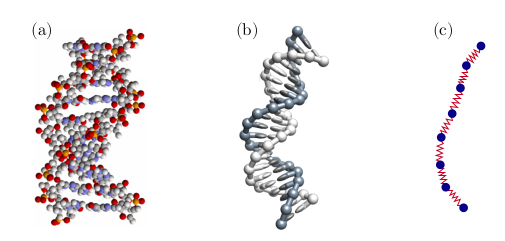
\includegraphics[width=0.6\linewidth]{Figures/CoarseGrained.png}
    \caption{zelf nog namaken met blender!!!}%
    \label{fig:Figures/CoarseGrained}
\end{figure}


\cleardoublepage
% \vspace{-1cm}
% \epigraph{Given for one instant an intelligence which could comprehend all
% the forces by which nature is animated and the respective positions
% of the beings which compose it, if moreover this intelligence were vast
% enough to submit these data to analysis, it would embrace in the same
% formula both the movements of the largest bodies in the universe and
% those of the lightest atom; to it nothing would be uncertain, and the
% future as the past would be present to its eyes.}
% {--- \textup{Pierre-Simon Laplace}}
\chapter{The DNA Nanopiston}

\begin{theo}[Chapter Reference]{thm:pythagoras}
  The contents of the chapter is based on:
  \vspace{-0.4cm}
  \begin{itemize}
    \item Bayoumi, M., Nomidis, S. K., Willems, K., Carlon, E., and Maglia, G. (2021).
      Autonomous and active transport operated by an entropic dna piston.\\
      Nano Letters, 21(1):762–768. PMID: 33342212.
  \end{itemize}
  \vspace{0.3cm}
\end{theo}

The DNA nanopiston is a molecular machine developed by the Maglia research group[.].  Its
main function constitutes the turning over of chemical fuel, in the form of ssDNA,  into
autonomous motion. The design is based upon the group earlier work, where they developed
a protein rotaxane[.], consisting of a polypeptide thread trapped in a Clya nanopore by
two stopper proteins. This rotaxane could be moved between two stable states inside the
nanopore by an electric potential, acting as a molecular switch.

Motivated by the results from this research, the DNA nanopiston was developed by Bayoumi
et al.[.] in the Maglia group. In this new molecular machine the rotaxane constitutes of
a DNA strand instead of a polypeptide thread. Utilising the thermodynamic transitions of
DNA, this complex is capable of actively transporting DNA cargo-strands through the
nanopore.

In this chapter the work of Bayoumi et al. is discussed, giving an overview of the
construction and operating cycle of this molecular machine.  At the end of this chapter
the molecular dynamics simulations from the paper of Bayoumi et al. are discussed, as
they where the main inspiration behind our project.

\section{Rotaxane Formation}


Synthetic molecular machines are often times embedded in larger complexes, providing the
necessary structure for their operation. For this reason biological nanopores are a
suitable starting point in the development of molecular machines. These transmembrane
proteins spontaneously self-assemble into well defined structures, embedded into a lipid
bilayer. Extensive research has been performed towards designing methods and tools to
tailor their structural and electrostatic properties for specific use cases, originally
focused on Ionic current spectroscopy. This large back catalogue of research can now be
employed into building out their utility as an ideal building block for membrane bound
molecular machines.

The design of the DNA nanopiston is centred around the biological nanopore Cytolysin
A (ClyA). A modified variant ClyA-AS is used, which has been specially engineered for
use in Ionic Current Spectroscopy.[.] By virtue of the large inner lumen of ClyA,
translocation of dsDNA through the pore is possible. The molecular machine utilises this
property by capturing a DNA rotaxane structure inside of the pore, anchoring it to the
lipid membrane. The rotaxane is composed of a DNA complex connected to two neutravidin
protein stoppers via biotin, which serve to keep the structure captured in the pore. The
DNA complex consists of three ssDNA strands: ssDNA $1$, ssDNA $2$, and ssDNA $3$, shown
in fig
....

The formation of the DNA nanopiston takes place in a saline filled reservoir, where a
ClyA nanopore is embedded into a membrane portioning the reservoir into a cis- and
trans-side. To start the formation process Neutravidin ($0.5\ \mu M$), ssDNA $1$
($5′-\text{biotinylated, }100\text{ nt, }1.2\ \mu M$) and ssDNA $2$ ($80\text{ nt, }1
\mu M$) are added to the cis-compartment. Since the first $70$ nucleotides of ssDNA $1$
are complementary to the last $70$ nucleotides of ssDNA $2$ both, the two strands will
partially hybridise. Resulting in an DNA duplex structure, on one side connected to a
neutravidin stopper and on the other two ssDNA overhangs.

Applying a voltage of $+100\ mV$ over the reservoir results in a net force guiding the
DNA complex from the cis towards the trans-side. The applied potential drives the
capturing of the DNA inside the nanopore, observed as a drop in the current through the
pore (Fig ..). The complex remains indefinitely captured inside the pore until the
applied potential is reversed, restoring the open-pore current.

Finally neutravidin ($1\ \mu M$) and ssDNA $3$ ($3\text{′-biotinylated, }20\text{ nt, }2
\mu\ M$) are brought into the solution at the trans-side, while keeping the potential at
$+ 100\ mV$. The longest overhang of the captured DNA thread is formed by the 30 free
nucleotides of ssDNA. The added strand, ssDNA $3$, is fully complementary with the last
$20$ nucleotides of this overhang, resulting in the hybridisation of both strands. To
verify if the hybridisation has successfully taken place, the voltage over the reservoir
is reversed. If no difference is measured in the pore-current, we conclude that the
stable structure is formed, capturing the rotaxane inside the pore by the two protein
stoppers.

After the hybridisation we find the final structure, which is referred to as the
rotaxane-ds. Here the suffix, $ds$, alludes to the predominately dsDNA composition of
this rotaxane configuration.\\


\begin{figure}[ht!]
  \begin{centering}
  \adjustbox{minipage=1.3em,valign=t}{\subcaption{}\label{sfig:testa}}%
  \begin{subfigure}[t]{\dimexpr.92\linewidth-1.3em\relax}
  \centering
  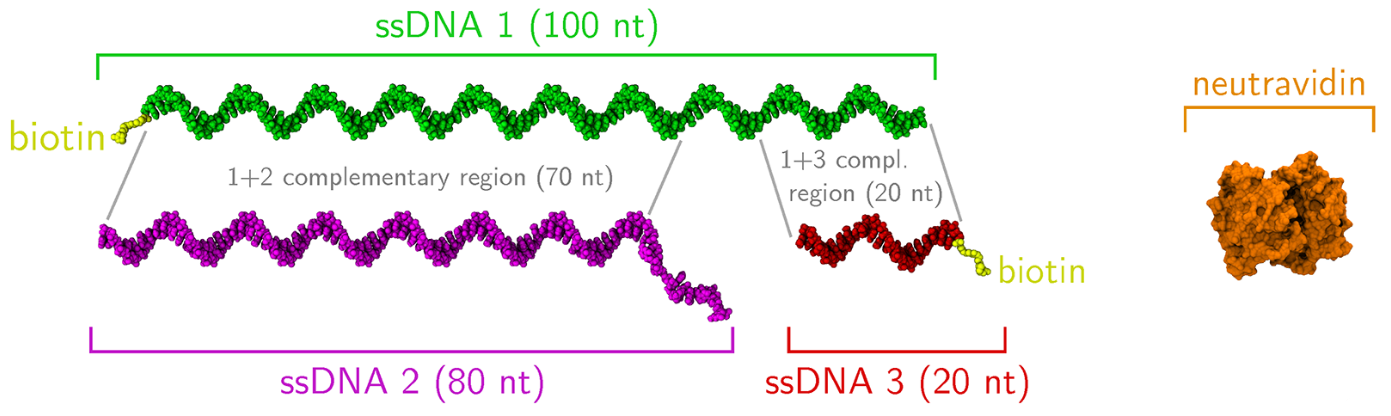
\includegraphics[width=\linewidth,valign=t]{Figures/RConstruction1.png}
  \end{subfigure}%
  \vspace{0.5cm}
  \adjustbox{minipage=1.3em,valign=t}{\subcaption{}\label{sfig:testa}}%
  \begin{subfigure}[t]{\dimexpr.92\linewidth-1.3em\relax}
  \centering
  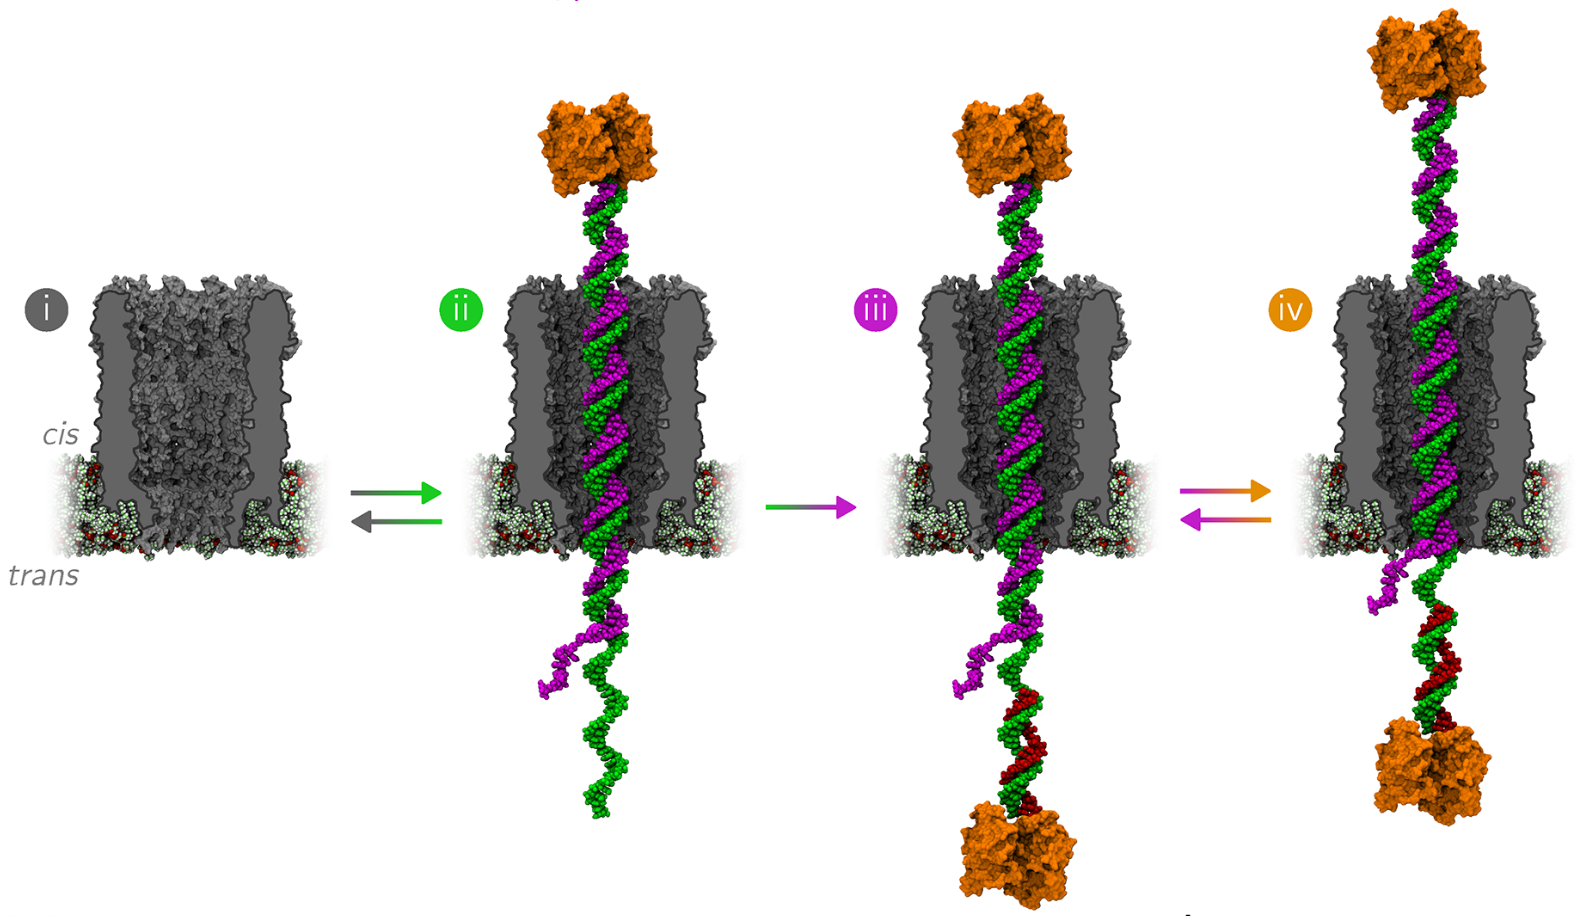
\includegraphics[width=\linewidth,valign=t]{Figures/RConstruction2.png}
  \end{subfigure}%
  \vspace{0.5cm}
  \adjustbox{minipage=1.3em,valign=t}{\subcaption{}\label{sfig:testb}}%
  \begin{subfigure}[t]{\dimexpr.92\linewidth-1.3em\relax}
  \centering
  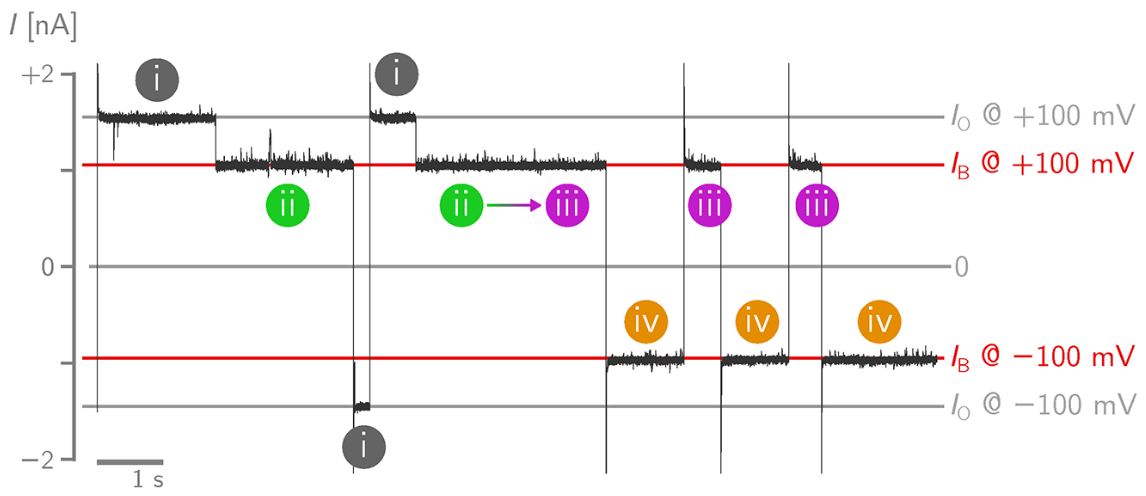
\includegraphics[width=\linewidth,valign=t]{Figures/RConstruction3.png}
  \end{subfigure}
  \caption{This is a figure [.]}
  \label{fig:test}
  \end{centering}
\end{figure}


\newpage

\section{Operating principles}

Once rotaxane-ds is formed, the addition of ssDNA 4 (0.5μM) to the trans chamber, which
is fully complementary to ssDNA 2, induces the displacement of the latter in trans via a
strand displacement reaction, using the ssDNA 2 overhang as a toehold (Figure 2)

During the strand displacement reaction, two possible transient states possibly occur.


the cis neutravidin is transiently pushed toward
the trans side, most likely entering the lumen of the nanopore (see Section S3).

The intermediate state of the strand displacement reaction can occur in two possible
ways. In the first scenario, the DNA cargo is hybridized with the fuel exclusively
outside the nanopore in the trans solution. This implies that neutravidin will enter
inside the lumen of the nanopore. Indeed, previous studies have shown that avidin can
enter the cis lumen of ClyA but cannot translocate through the nanopore. Alternatively,
the strand displacement reaction can  take place inside the nanopore. In this case, the
DNA transport would occur from trans-to-cis rather than from cis-to-trans, as described
in the main text. We think this is unlikely, because this scenario would require the
translocation through the trans entry of three DNA strands


After the removal of ssDNA 2,
a new configuration is obtained, in which ssDNA1 and ssDNA3 remain trapped within the
pore. This configuration consists ofa 90-base-ssDNA thread on the cis end, a
10-basepair-dsDNA stretch on the trans side, and neutravidin on both sides ofthe pore
(Figure 2). We refer to this configuration as rotaxane-ss.

The subsequent addition of 0.5 μM ofssDNA 2 cargo to the cis side restores rotaxane-ds,
as ssDNA 2 hybridizes with the thread of rotaxane-ss

After each cycle, one cargo molecule is transported from cis to trans and one fuel
molecule is expended.

These cycles were found to be both at positive, + 20 mV (Figure 2a, top trace), + 50 mV
and +100 mV (Figure S3), and negative, − 20 mV (Figure 2a,
bottom trace), biases. Higher negative applied potentials (e.g., −50 mV, Figure S3)
prevented the cycling

The working of the nanopiston against and with external bias is important, postulated
that it is due to the entropic interaction between the rotaxane and the pore.
Discuss the importance of entropy. power stroke is toehold disp reaction. Results in lwo
entropy state. This entropic energy provides the recovery stroke. Next hybridisation with
the fuel strand makes us come back to the intial configuration.

Furthermore, the cycles were faster at positive than at negative applied potentials, but
were slower as the potential was increased. This voltage dependency can be explained by
toehold sequestering inside the nanopore

Due to brownian motion both autonomous and non-autonomous systems use ratcheting to
eventually deliver work. Using this method minimal synthetic machines can deliver
elegance and performance shedding the 'baggage' of biological evolution.

Figure 2.2a shows the measured current over through the nanopore during the operation
cycle. The ionic current of rotaxane-ss is lower than the blocked current ofrotaxane-ds
most likely reflecting the coiled structure of ssDNA inside the nanopore. Shows the
limitation of the experimental analysis of the pore, only view into the system is
throught the measured current. To get a more indepth understanding of the conformal
fluctuations of the pore computation analysis was performed in the form of molecular
dynamics simulations.


% Dit nog ergens bij schrijven idk waar, maar deze krachten zijn wel belangrijk?
% misschien bij de biological nanopores.
% Electrophoretic, electro-osmotic and entropic forces are, in principle, acting on the
% rotaxanes. The electrophoretic force sets the negatively charged DNA in motion, under the
% action of the applied bias (from cis to trans for
% ∆?? > 0 ). Electroosmosis generates an opposing force, arising from the motion of cations
% accumulated on the walls of the negatively charged ClyA pore and the DNA thread. Finally,
% the entropic force is solely geometry specific, and pushes the rotaxane towards
% conformations with high configurational entropy. Entropic forces are expected to play an
% important role in the rotaxanes studied here, which are composed of stiff dsDNA and
% flexible ssDNA parts.



\begin{figure}[ht]
  \begin{centering}
  \adjustbox{minipage=1.3em,valign=t}{\subcaption{}\label{sfig:testa}}%
  \begin{subfigure}[t]{\dimexpr.95\linewidth-1.3em\relax}
  \centering
  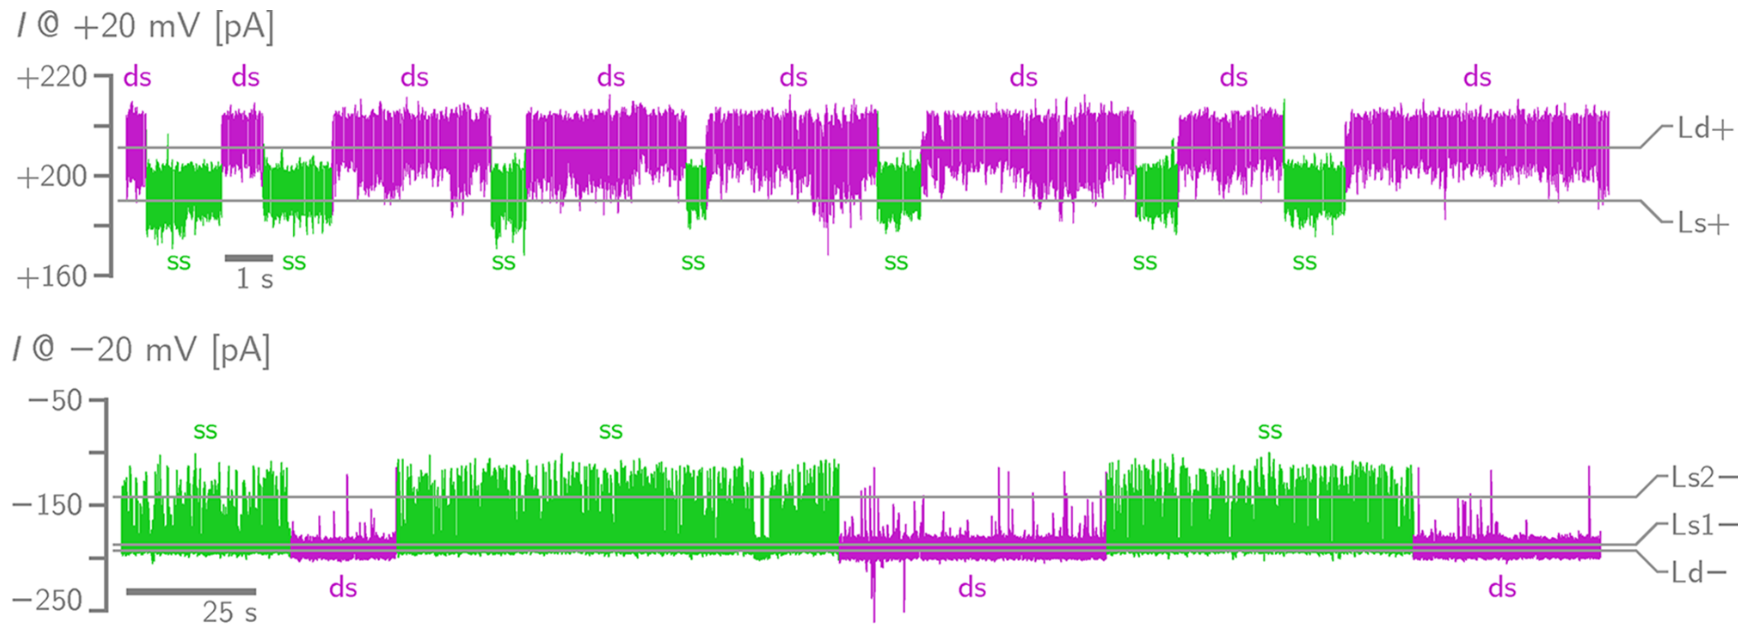
\includegraphics[width=\linewidth,valign=t]{Figures/FluctuationRotaxane.png}
  \end{subfigure}%
  \vspace{0.5cm}
  \adjustbox{minipage=1.3em,valign=t}{\subcaption{}\label{sfig:testb}}%
  \begin{subfigure}[t]{\dimexpr.5\linewidth-1.3em\relax}
  \centering
  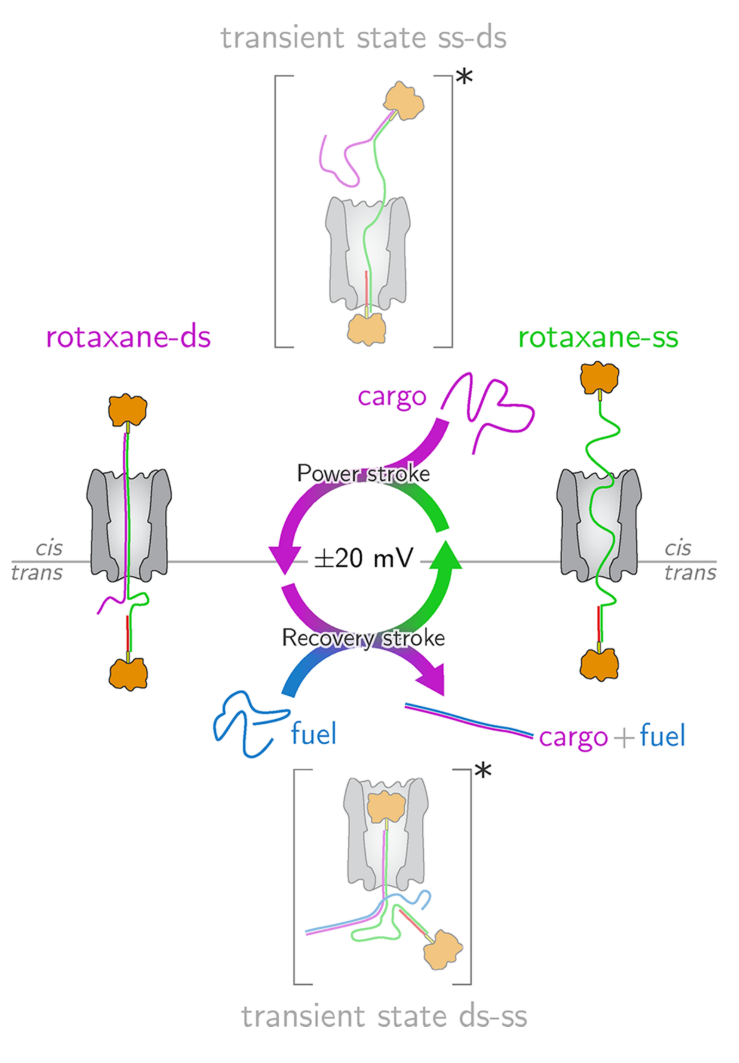
\includegraphics[width=\linewidth,valign=t]{Figures/RotaxaneCycle.png}
  \end{subfigure}
  \caption{This is a figure}
  \label{fig:test}
  \end{centering}
\end{figure}

\section{Coarse-grained simulations}

\begin{figure}[h]
  \centering
  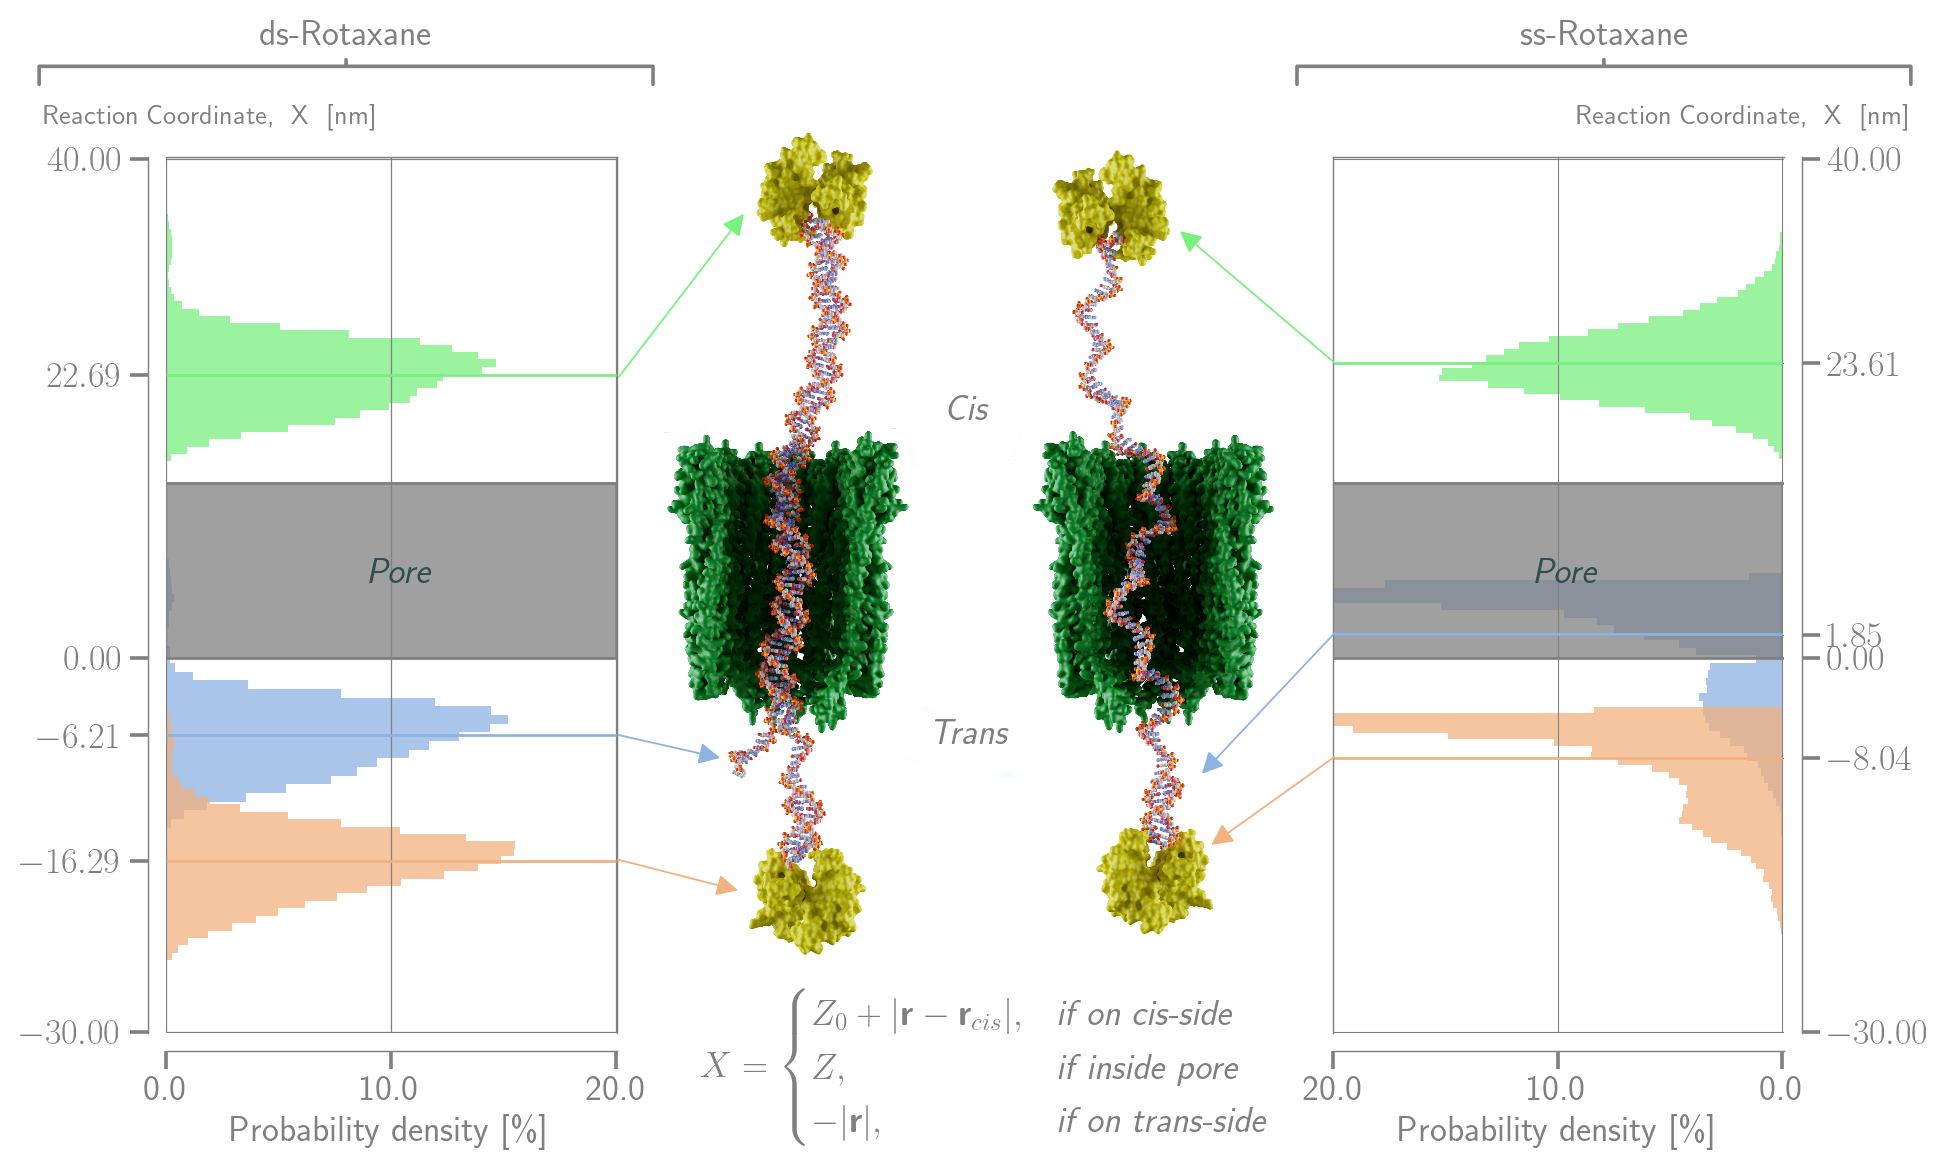
\includegraphics[width=0.8\linewidth]{Figures/RotaxaneFluctuations.png}
\end{figure}


\chapter{Improving the Model}
\vspace{-1cm}
\epigraph{All models are wrong, but some are useful.}
{--- \textup{George Box}}
\section{OxDNA}

\begin{wrapfigure}{r}{0.45\textwidth}
  \begin{center}
    \includegraphics[width=0.42\textwidth]{Figures/oxDNA_model.png}
  \end{center}
  \caption{Structure of the OxDNA model with the different interactions.
          Figure was taken form [].}
\end{wrapfigure}

OxDNA is a coarse-grained model of DNA developed by Thomas E. Ouldridge et al. at Oxford
university. The central aim of the project was to develop a coarse-grained model of DNA
that could be used in the design of DNA technology. For the development of these
technologies a model was needed that accurately captured the structural, mechanical and
thermodynamical properties of DNA while keeping the computational cost low.

The OxDNA model represents each nucleotide in the DNA strand as a rigid unit. Each rigid
nucleotide has three independent interaction sites, each capturing a different aspect of
the model. The interactions between these pseudo atoms are next compared to experimental
data to tweak the interactions, characterising the approach as "top down"
coarse-graining. The interactions defined in the OxDNA model can be summarized as,

\begin{equation}
  \begin{aligned}
    V = \sum_{\text{nearest neighbours}} \bigg[ V_{\text{backbone}} + V_{\text{stack}} +
    V^{'}_{\text{exc}}\bigg]\\
    + \sum_{\text{other pairs}} \bigg[V_{\text{HB}} + V_{\text{cross stacking}} +
    V_{\text{exc}} + V_{\text{coax stack}}\bigg].
  \end{aligned}
\end{equation}

The first interaction site is the hydrogen-bonding/base excluded volume site,
incorporating the hybridisation of complementary nucleotides into the model. The
hydrogen-bonding interactions are not fixed, allowing for OxDNA to simulate dsDNA, ssDNA
and their thermodynamic transitions.

The second interaction site is an excluded volume interaction located at the backbone.
These interactions simulate the covalent bonding between consecutive phosphate groups
using the FENE (finitely extensible nonlinear elastic) bond type.

The last interaction site is again located at base where it provides a base stacking
interaction between consecutive nucleotides. The nucleotides stacking in DNA is crucial
for the formation of the characteristic helical structure. Using these stacking
interactions this structure is implicitly imposed in the model. Contrasting the common
approach of explicitly imposing the Double helix structure in other coarse grained-models
like 3SPN and Martini. This implicit structure allows for the unstacking of nucleotides,
which especially in ssDNA is an important contribution to the flexibility of the strand.

During the simulations of the DNA Nanopiston both the flexibility of the single stranded
DNA strands and the hybridisation reactions play an important role. Since both of these
aspect of DNA are accurately captured by the OxDNA model, it provides a logical choice
for our simulations. The low number of degrees of freedom in the model, allows us to
simulate computationally intensive simulations like DNA hybridisation.

\section{DNA Thermodynamics}

 The field of DNA thermodynamics focuses on understanding how the structure of DNA varies
with temperature. Due to the nature of hydrogen bond interactions, that give rise to the
structure of dsDNA, the association and dissociation of the DNA duplex is possible. The
former is called DNA hybridisation shown in fig. ..., driven by a reduction in free
energy due to the bonding of complementary base-pairs. The latter is called DNA
melting, a process observed at high temperatures. This dissociation is
energetically driven, since the reduction in free energy due to base-pair hybridisation
is no longer a favourable trade-off with the reduction in configurational entropy in the
duplex structure.

During the discussion of the DNA nanopiston, we stated that thermodynamic transitions of
DNA are the driving force behind its operating cycle. The power stroke of the piston is
induced by a toehold mediated strand displacement reaction, while a hybridisation
reaction facilitates the recovery stroke.

Initiating a hybridisation reaction between two strands of ssDNA incurs a thermodynamic
penalty. This penalty originates in the decrease of configurational entropy, when the
strands start to form a duplex. This has a consequence that initial contacts in these
reactions often dissociate, due to the initial energy barrier that needs to be crossed
before the full hybridisation becomes energetically favourable. Even when an initial
contact
results in the stabilisation of a dsDNA duplex for select base-pairs, the configuration
often times is not conducive to full duplex formation. Especially in repetitive
sequences, the chance of a mismatched initial hybridisation is significant.

Another limiting factor to the rate constant of hybridisation reactions is that these
transitions are not characterised by a single state, but rather by an ensemble of
possible transition pathways. The number of pathways increase dramatically when the
strand sequences are repetitive, giving rise to hybridisation pathways facilitated by
Inchworm and pseudo-knot displacements[.].

The combination of the unstable initialisation of hybridisation reactions together
with its many transition pathways, complicates the analysis of the full reaction kinetics
observed in DNA hybridisation.


\begin{figure}[ht]
  \begin{centering}
  \adjustbox{minipage=1.3em,valign=t}{\subcaption{}\label{sfig:testa}}%
  \hspace{-0.3cm}
  \begin{subfigure}[t]{\dimexpr.2\linewidth-1.3em\relax}
  \centering
  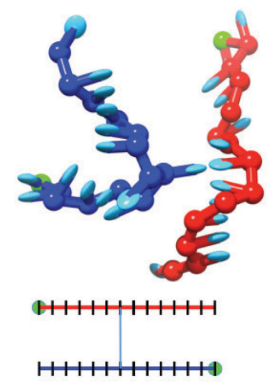
\includegraphics[width=1.06\linewidth,valign=t]{Figures/hybridDiag1.png}
  \end{subfigure}%
  \adjustbox{minipage=1.3em,valign=t}{\subcaption{}\label{sfig:testa}}%
  \hspace{-0.35cm}
  \begin{subfigure}[t]{\dimexpr.2\linewidth-1.3em\relax}
  \centering
  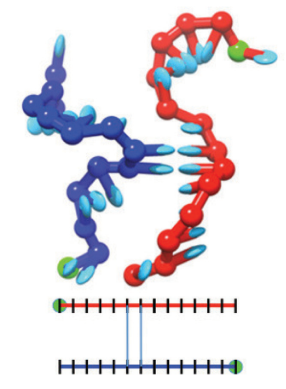
\includegraphics[width=1.09\linewidth,valign=t]{Figures/hybridDiag2.png}
  \end{subfigure}%
  \adjustbox{minipage=1.3em,valign=t}{\subcaption{}\label{sfig:testb}}%
  \hspace{-0.28cm}
  \begin{subfigure}[t]{\dimexpr.2\linewidth-1.3em\relax}
  \centering
  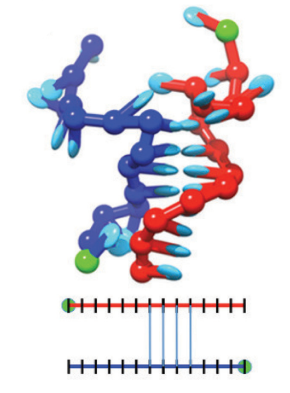
\includegraphics[width=1.1\linewidth,valign=t]{Figures/hybridDiag3.png}
  \end{subfigure}
  \adjustbox{minipage=1.3em,valign=t}{\subcaption{}\label{sfig:testa}}%
  \hspace{-0.21cm}
  \begin{subfigure}[t]{\dimexpr.2\linewidth-1.3em\relax}
  \centering
  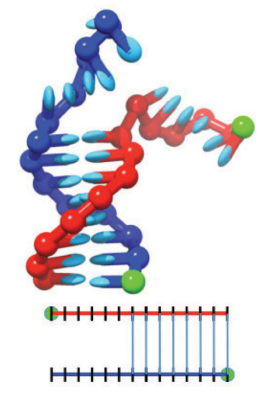
\includegraphics[width=.98\linewidth,valign=t]{Figures/hybridDiag4.png}
  \end{subfigure}%
  \adjustbox{minipage=1.3em,valign=t}{\subcaption{}\label{sfig:testa}}%
  \hspace{-0.38cm}
  \begin{subfigure}[t]{\dimexpr.2\linewidth-1.3em\relax}
  \centering
  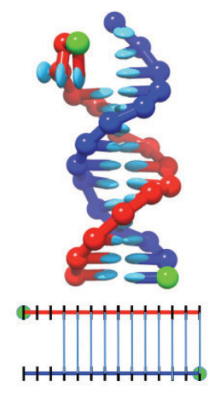
\includegraphics[width=.8\linewidth,valign=t]{Figures/hybridDiag5.png}
  \end{subfigure}
  % \adjustbox{minipage=1.3em,valign=t}{\subcaption{}\label{sfig:testb}}%
  % \hspace{-0.5cm}
  % \begin{subfigure}[t]{\dimexpr.2\linewidth-1.3em\relax}
  % \centering
  % 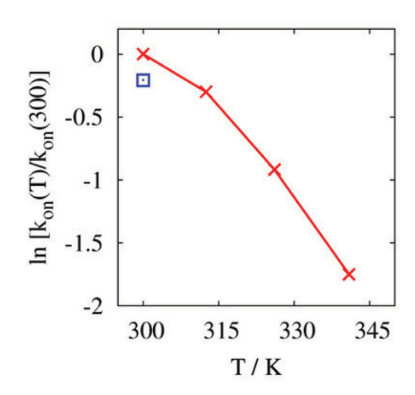
\includegraphics[width=1.5\linewidth,valign=t]{Figures/hybridDiag6.png}
  % \end{subfigure}
  \caption{This is a figure [.]}
  \label{fig:test}
  \end{centering}

\end{figure}

% ‘fraying’ to describe the disruption of base-pairs at the end of a duplex; if all base
% pairs fray, the duplex melts or dissociates.
%
% ‘zippering’ refers to when a new base-pair forms at the end of an existing duplex, shown
% in figure 3.2

The other important thermodynamic transition in the operating cycle of the nanopiston
is a toehold mediated strand displacement. Initially this reaction consists out of two
components. The first is an imperfect duplex structure, formed by a substrate strand and
an incumbent strand. The two strands are partially complementary by having either a
mismatch in their base-pair sequence or a surplus of base-pairs on the substrate strand.
The non-hybridised part of the substrate constitutes a flexible strand of ssDNA
that is referred to as the toehold.

The second component is called the invasive strand, and is fully complementary with the
substrate. It is energetically favourable for the invading
strand to disrupt the imperfect duplex structure and form a fully Watson–Crick
complementary dsDNA with the substrate strand. This displacement reaction results in an
overall reduction in the free energy of the system, since the strand displacement
increases the total number of hybridised base-pairs.

The process of strand displacement starts with the hybridisation of the toehold and the
invading strand. Once this initial hybridisation has occurred the invading strand can
start to contest hybridised base-pairs of the imperfect duplex. Disrupting the
base-pairing of the duplex is referred to as fraying, while the reverse process
where new base-pairs are formed is called zippering. During this process the invading
strand competes with the incumbent strand to form base-pairs with the substrate.

The reaction can be modelled using an one-dimensional energy landscape, called the
intuitive energy landscape (IEL) model[.], shown in figure ... . In the shape of the
energy landscape we recognise two distinct features. The first features is the initial
energy barrier, also seen in DNA hybridisation. This energy barrier again arises from a
reduction in configurational entropy, when the initial binding happens. The second
feature
is the plateau, representing the change in free energy when the strand
displacement takes place. This plateau gives rise to a relatively slow reaction, which
can be explained using a simple toy model. Considering a scenario, where the substrate
consists of $N+1$ nucleotide, with only one of these nucleotides constituting the
toehold. If we now assume that both the incumbent and invasive strand contest each others
hybridised base-pairs at the same rate, the displacement reaction can be modelled as a
random walk. The model is reduced to a famous problem in probability theory, called the
gamblers ruin. It can be shown that the reaction rate scales as $1/3N$[.], making the
Toehold displacement reaction increasingly difficult to study for large strands.

These two types of thermodynamic transitions, central in the operation cycle of the DNA
nanopiston, are relatively difficult to study due to their slow reaction rates and
initial energy barrier. Accurately analysing the reaction kinetics of these rare events,
requires the use of advanced sampling techniques.

\begin{figure}[ht]
\begin{center}
  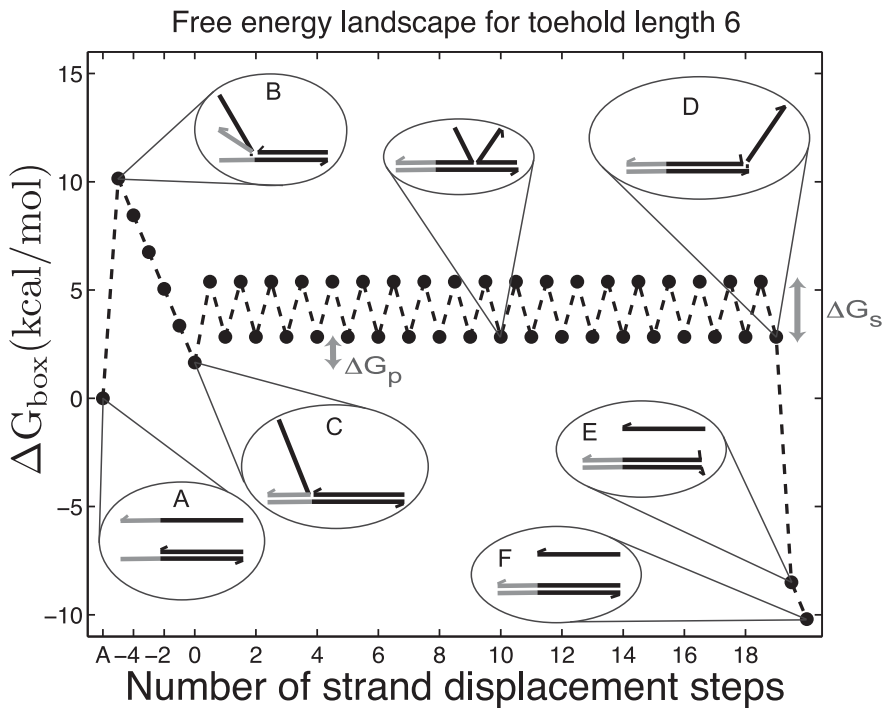
\includegraphics[width=0.6\textwidth]{Figures/ToeholdDiagram.png}
  \caption{write caption[.]}
\end{center}
\end{figure}



\section{Forward Flux sampling}

Computational methods are used to study a wide variety of phenomena, ranging from
large meteorological events to chemical reactions at the atomic scale. One class of
phenomena that is omnipresent in all these fields are the rare events. A rare event is an
event caused by stochastic fluctuations in the system, characterised by a large
gap in the time-scales of the duration of the events and their temporal spacing.
The infrequency of their occurrence in combination with their short duration, makes them
hard to study with both experimental and computational approaches.

Using this definition many natural processes can be classified as rare events, among
which the hybridisation and toehold displacement reactions studied in this thesis. Due to
the large temporal spacing of these rare events, brute-force molecular dynamics
simulations would simulate a lot of wait time between events. To effectively probe the
kinetics of these rare events, advanced sampling methods are needed.

A large ensemble of advanced sampling methods have been developed and can be largely
divided into two classes. The first class are the free energy methods, based upon
applying a biasing potential onto chosen collective variables. These potentials bias the
Hamiltonian of the system in such a way that rare parts of its configuration space are
explored. Notable examples of these methods are adaptive biasing force algorithm[.],
basis function sampling[.] and umbrella sampling[.]. %(SSAGES)

The second class of methods, known as path sampling methods, do not influence the
systems Hamiltonian, but rather interface directly with the simulations trajectories. The
transition path ensemble is usually sampled by perturbing an initial transition path or
partitioning the phase space in subregions. Examples of these methods are transition
path sampling [.] and forward flux sampling[.][.].  The latter will be used in our
hybridisation simulations, motivated by its relative simplicity.

Forward Flux Sampling (FFS) starts with identifying two local minima, $A$ and $B$, in the
energy landscape of our system, for which we want to sample the transition path ensemble.
Next an order parameter, $\lambda(x)$, is defined with the aim of partitioning the
phase space, $\Omega$, using a set of nonintersecting hypersurfaces. By design, we
choose this order parameter to be a function, $\lambda(.):\ $\Omega$\ \rightarrow
\mathcal{R}$, monotonically increasing from the initial state $A$ and too the final
state $B$.

Using this function the two local minima can
now be specified as $A := \{x: \lambda(x) < \lambda_A\} $ and $B := \{x: \lambda(x) \geq
\lambda_B\} $. The chosen levels of order, $\lambda_A$ and $\lambda_B$, construct the
interfaces separating the two local energy basins from the rest of the
phase space. Finally this procedure can be done for a $N$-number of interfaces
partitioning the space between $A$ and  $B$, we find
\begin{equation}
\lambda_A = \lambda_0 < \lambda_1< \dots < \lambda_{N-1} < \lambda_N = \lambda_B
\end{equation}
Note that this methods does not require an in depth knowledge of the systems energy
landscape, however the choice of order parameter will heavily influence the
efficiency of the simulation. Analogues to the ambiguous choice of a collective variable
in free energy methods, making these decisions is often more an art then a science.

The ultimate aim of these methods is to get a grasp of the kinetics of rare events. In
quantitative terms this means determining the rate constant of the transition
from $A$ to  $B$, denoted as $k_{AB}$. The expression used to calculate $k_{AB}$ is:
 \begin{equation}
    k_{AB} = \frac{\langle \Phi_{A,n} \rangle}{\langle h_{\mathcal{A}}\rangle} =
    \frac{\langle \Phi_{A,0} \rangle}{\langle h_{\mathcal{A}}\rangle}
    P(\lambda_n|\lambda_0)
 \end{equation}
 where $\langle \Phi_{A,n} \rangle$ is the steady-state flux of trajectories starting in
 $A$ and reaching the final interface $\lambda_n$ (i.e. reaching B) and
$\langle h_{\mathcal{A}}\rangle$ is the average fraction of time that  a trajectory
spends in the basin of local minima $A$. In the above equation this steady state flux is
factorised into the flux of trajectories starting in $A$ and crossing $\lambda_0$ and the
subsequent probability of reaching the final state from this
interface. Using the previously defined interfaces, we can now factorize the events'
probability into transition probabilities between the individual interfaces as
\begin{equation}
    P(\lambda_n|\lambda_0) = \prod_{i=0}^{n-1} P(\lambda_{i+1}|\lambda_i).
 \end{equation}
Estimating these transition probabilities can be done by shooting trajectories starting
from one interface to the next, while keeping track of the fraction of attempts
successfully crossing the next interface. Since not the entire energy landscape between
the minima has to be crossed, measuring these small transitions can be more easily done.

Note that this set-up allows for simulations of both equilibrium and out-of-equilibrium
systems, it does not require detailed balance like other sampling techniques. Non
equilibrium systems are ubiquitous in soft matter physics, illustrating another strength
of the method.
\begin{figure}[ht]
\begin{center}
  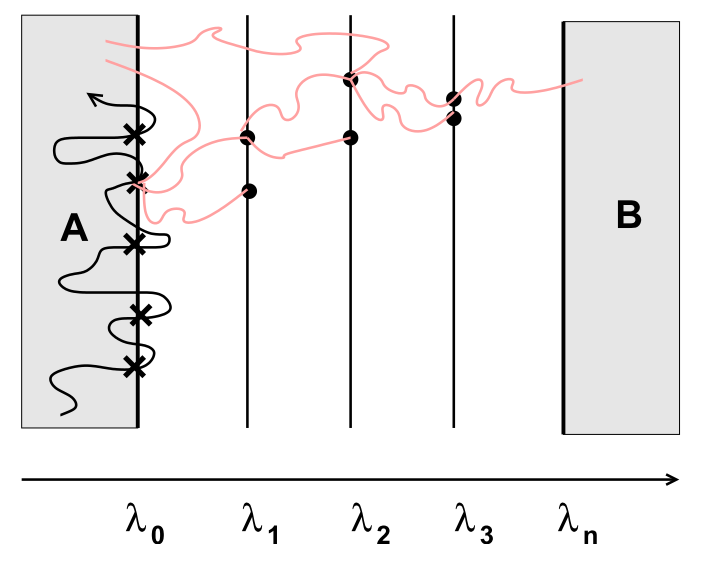
\includegraphics[width=0.5\textwidth]{Figures/FFS.png}
  \caption{write caption[.]}
\end{center}
\end{figure}
Different variants on the FFS method have been devised, they differ in the approach by
which they calculate the probability $P(\lambda_n|\lambda_0)$. During this thesis I
choose to use the “Rosenbluth-like” (RB) method [zie citation allen review]. The choice
is motivated
by its resemblance with well known Monte Carlo Simulations and recursive nature, making
it easy to implement.  This method generates unbranched transition paths from state $A$
to state $B$, making them easy to analyse. The algorithm is described in six steps:
\begin{enumerate}[label=\textbf{(\roman*)}]
   \item Generate configurations on the $\lambda_0$ interface by running
      simulations in the $A$ basin. Keeping track of the fractions $\langle
      \Phi_{A,0} \rangle/\langle h_{\mathcal{A}}\rangle$ is evaluated.
   \item Fire $k_0$ trial runs from generated configurations on $\lambda_0$ until they
      cross $\lambda_1$ or cross back to $\lambda_0$. Store the final configurations of
      the successful simulations.
   \item Sample one of the saved configuration on the $\lambda_1$ interface and use it to
      shoot $k_1$ runs to the next interface $\lambda_2$.
   \item Iterate the previous steps until the trajectories reach $\lambda_n$ or no more
     configurations are available.
   \item If not successful, sample a stored configuration on $\lambda_0$ and repeat the
      steps $\textbf{(i)}$ to $\textbf{(iv)}$.
   \item Finally compute $P(\lambda_n|\lambda_0)$ using a weighted average of individual
     transition probabilities as described below.
\end{enumerate}
Calculating the transition probabilities is done by taking a weighted average of the
attempted trial runs. The path $b$ starting at the inital basin and reaching
interface $\lambda_i$ is assigned a weight $w_{i,b}$ as
\begin{equation}
   w_{i,b} = \prod_{j=0}^{i-1} S_{j,b}/k_j,
\end{equation}
where $S_{j,b}$ is the number of successful trajectories crossing interface $j$ during
the generation of path $b$. Using these weights, the transition probability is computed
using
\begin{equation}
   P(\lambda_{i+1} | \lambda_i) = \frac{\sum_{b} w_{i,b}\ S_{i,b}/k_i}{\sum_b w_{i,b}}.
\end{equation}


\section{Computational Setup}

The model used to study the DNA nanopiston in this thesis, is largely based on the model
previously devised by Bayoumi et al. The main variation between the two models lays in
the different coarse-grained models, used to simulate the DNA strands. As discussed in
Chapter 2, the Bayoumi model uses a bead-spring approach to simulate DNA strands, where
we use the more sophisticated oxDNA model. This DNA model gives a better
representation of the dynamics of DNA strands, at the same time allowing for accurate
simulations of the thermodynamic transitions in the DNA nanopiston.

Our simulations are performed using the popular molecular dynamics simulator,
LAMMPS.\cite{PLIMPTON19951} Employing the LAMMPS implementation of oxDNA developed by
Henri et al.,
it becomes possible to study the interactions between oxDNA strands and externally
defined particles.\cite{Henrich18} The initial configurations of the simulations are
generated using the
Moltemplate package, a general purpose molecule builder for LAMMPS.\cite{JEWETT2021}

The molecular dynamics simulations performed in this thesis utilises a Langevin
thermostat, more precisely the Dot-C Langevin integrator, also implemented by Henri et
al. This is a LAMMPS implementation of the “Langevin C” integrator developed by
Davidchack et al., falling in the class of rigid-body Langevin-type
integrators.\cite{Davidchack2015}
This type of thermostat separates the stochastic and deterministic parts of a Langevin
thermostat to efficiently take into account the extra degrees of freedom in the system,
arising from the non-spherical shape of the oxDNA beads. As is common practice in MD
simulations, the diffusion coefficient of the oxDNA strand is chosen larger then the
value of physical DNA. This is done to speed up the simulations, while ensuring its
physical accuracy.

The model is used to more accurately study the conformational fluctuations of
the DNA rotaxanes and develop understanding of the entropic interactions between the DNA
and the nanopore. Next the thermodynamic transitions in the operation cycle of the piston
are simulated using a forward flux sampling algorithm. The FFS algorithm is implemented
as a Python script, performing the simulations by interfacing with the Python API of
LAMMPS.


\chapter{Simulations of the Rotaxane}
\vspace{-1cm}
\epigraph{The career of a young theoretical physicist consists of treating the harmonic
oscilator in ever-incresing levels of abstraction.}
{--- \textup{Sidney Coleman}}
\vspace{2cm}
\noindent In this chapter the results of various simulations utilising the OxDNA based
rotaxane model are presented. The aim of this computational analysis is to shed light on
the entropic effects which play a central role in the nanopiston's operating cycle. By
extension, the thermodynamic transitions providing the free energy governing its
operation are studied.\\\\
To better understand the entropic interactions between the DNA rotaxane and the nanopore
a specially engineered rotaxane variant is studied. This other class of rotaxane is
called the mixed rotaxane, composing of different ds- and ssDNA fractions in an attempt
to isolate the influence of entropic interactions. Having explored the effects of the
entropic contributions, next the conformational fluctuations of the nanopiston are
simulated and analysed. Lastly, an attempt is made to simulate the thermodynamic
transitions driving the piston cycle. These particular simulations are made possible
by the use of a forward flux sampling algorithm.

\newpage

\section{Mixed Rotaxane}

Having identified the entropic interactions as key component of the nanopiston cycle,
studying them is an important but challenging task. The problem arises when we aim to
specify the entropic contributions to the conformal fluctuations of the rotaxane. The
main factor complicating this analysis is the multiplicity of the interactions acting
upon the nanopiston.\\

% Studying solely the contributions of entropic interactions in the conformal
% fluctuations  of the rotaxane is challenging task. The main factor complicating this
% analysis is the  multiplicity of the interactions acting upon the nanopiston.\\

The first category of forces is composed of the external forces arising from the
potential difference applied over the membrane. This potential difference induces an
electric field both outside and inside of the nanopore, influencing the movement of
molecules in these regions. The most significant contributions can be identified as the
electrophoretic and electro-osmotic forces acting upon the rotaxane. The second class of
forces is composed of the intrinsic forces. These forces do not arise from the
electric field, but rather originate from the direct interactions between the rotaxane
and the nanopore itself. Under this category fall the electrostatic, steric and entropic
forces, limiting the conformational freedom of the piston.



% Since both the DNA polymer and the ClyA nanopore have a net negative
% charge, the first intrinsic force can be identified as the electrostatic interaction
% between these two components of the piston. At short distances however this electrostatic
% force is dominated by the repulsive component of van der Waals forces arising from
% overlapping of the atoms' electron clouds. This contribution is referred to as the steric
% force. Lastly the entropic force is also categorised as a intrinsic force, arising from
% the reduction in available configurational micro states of the rotaxane upon confinement
% in the pore. [.]

In order to study the role of entropy in the conformational fluctuations of
the nanopiston, these effects need to be isolated from the other contributions present in
the system. To achieve this Bayoumi et al. devised a new variation of the rotaxane
called the mixed rotaxane. In this rotaxane variation the toehold is removed, resulting
in a thread composed of solely ds- and ssDNA. By varying the DNA composition of this
rotaxane the changes in entropic interactions can be analysed. More specifically, the
total length of the rotaxane was constant, i.e. the total number of nucleotides and
basepairs are fixed at 100, while the ssDNA part was varied from $0nt$ to $30 nt$ in
steps of $10nt$. The effects of these changes in composition were first studied using I-V
measurements in the range of $[-100mV, +100mV]$. During an I-V measurement a range of
voltages is applied over the lipid membrane and at each step in this voltage sweep the
current through the pore is measured. A detailed explanation of this method is described
in. \cite{MAGLIA2010591} The results from these experiments are presented in Figure....

The mixed rotaxane composed entirely of dsDNA yields an almost linear I-V trace in the
measured voltage range. This result indicates a constant obstruction of the nanopore over
the entire voltage sweep. On the other hand, the mixed rotaxane composed of a $10nt$
ssDNA strand shows a drastically different I-V trace. Decreasing the voltage below
$-20mV$ results in current fluctuations between two distinct levels. A second transition
can be observed when the voltage is further decreased below $-70mV$. Here the measured
current becomes independent from the applied voltage, suggesting a partial blockage of
the current through the nanopore. These same characteristics can be identified in the I-V
trace of
the mixed rotaxane with a $20nt$ ssDNA strand. Remarkably, the voltage range
in which the current fluctuations are observed is moved to a more negative
voltage range from $-30mV$ to  $-85 mV$. When the fraction of ssDNA in the mixed rotaxane
is further increased to $30nt$, the characteristic blockage is no longer observed and the
linear I-V trace is recovered.

\begin{figure}[ht!]

  \begin{centering}
  \adjustbox{minipage=1.3em,valign=t}{\subcaption{}\label{sfig:testa}}%
  \begin{subfigure}[t]{\dimexpr.29\linewidth-1.3em\relax}
  \centering
  \vspace{0.35cm}
  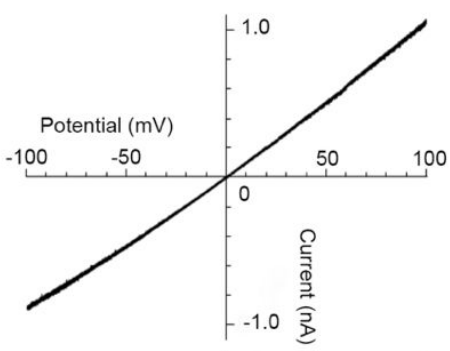
\includegraphics[width=1.05\linewidth,valign=t]{Figures/IV-100.png}
  \end{subfigure}%
  \adjustbox{minipage=1.3em,valign=t}{\subcaption{}\label{sfig:testb}}%
  \begin{subfigure}[t]{\dimexpr.5\linewidth-1.3em\relax}
  \centering
  \hspace{-0.2cm}
  \vspace{0.1cm}
  \includegraphics[width=0.95\linewidth,valign=t]{Figures/MR-100.png}
  \end{subfigure}%
  \adjustbox{minipage=1.3em,valign=t}{\subcaption{}\label{sfig:testc}}%
  \begin{subfigure}[t]{\dimexpr.21\linewidth-1.3em\relax}
  \centering
  \vspace{0.3cm}
  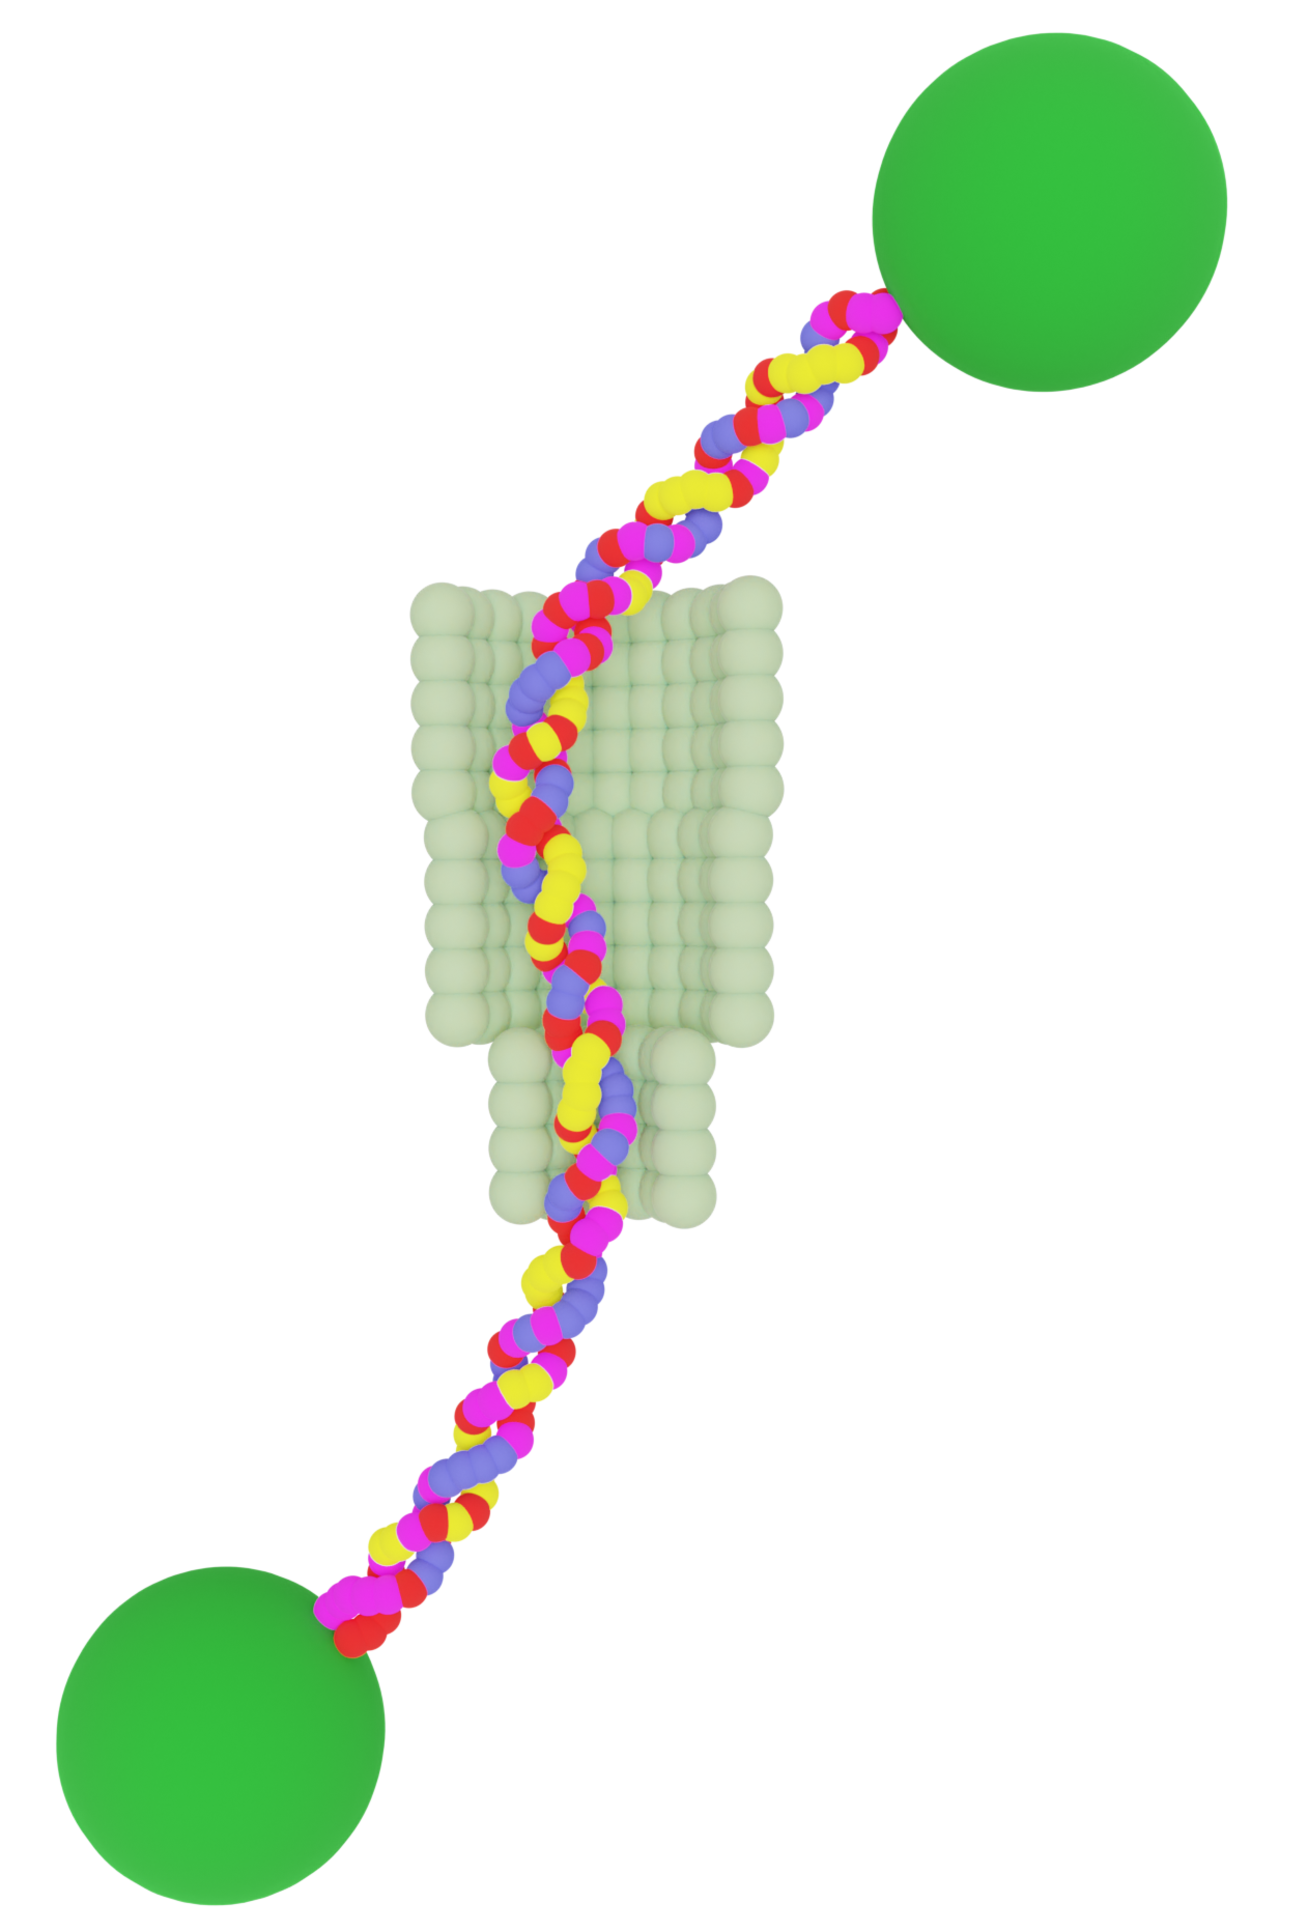
\includegraphics[width=0.8\linewidth,valign=t]{Figures/Rotaxane-100.png}
  \end{subfigure}
  \label{fig:test}
  \end{centering}

  \vspace{0.05cm}

  \begin{centering}
  \adjustbox{minipage=1.3em,valign=t}{}%
  \hspace{.35cm}
  \begin{subfigure}[t]{\dimexpr.3\linewidth-1.3em\relax}
  \centering
  \vspace{-0.1cm}
  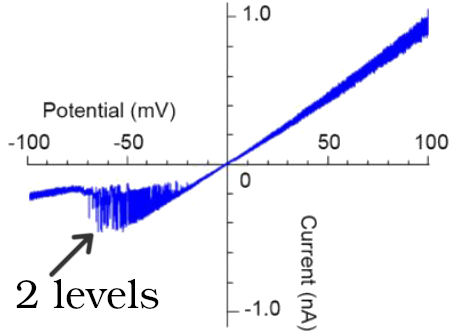
\includegraphics[width=1.05\linewidth,valign=t]{Figures/IV-90.png}
  \end{subfigure}%
  \adjustbox{minipage=1.3em,valign=t}{}%
  \hspace{.25cm}
  \vspace{-0.2cm}
  \begin{subfigure}[t]{\dimexpr.5\linewidth-1.3em\relax}
  \centering
  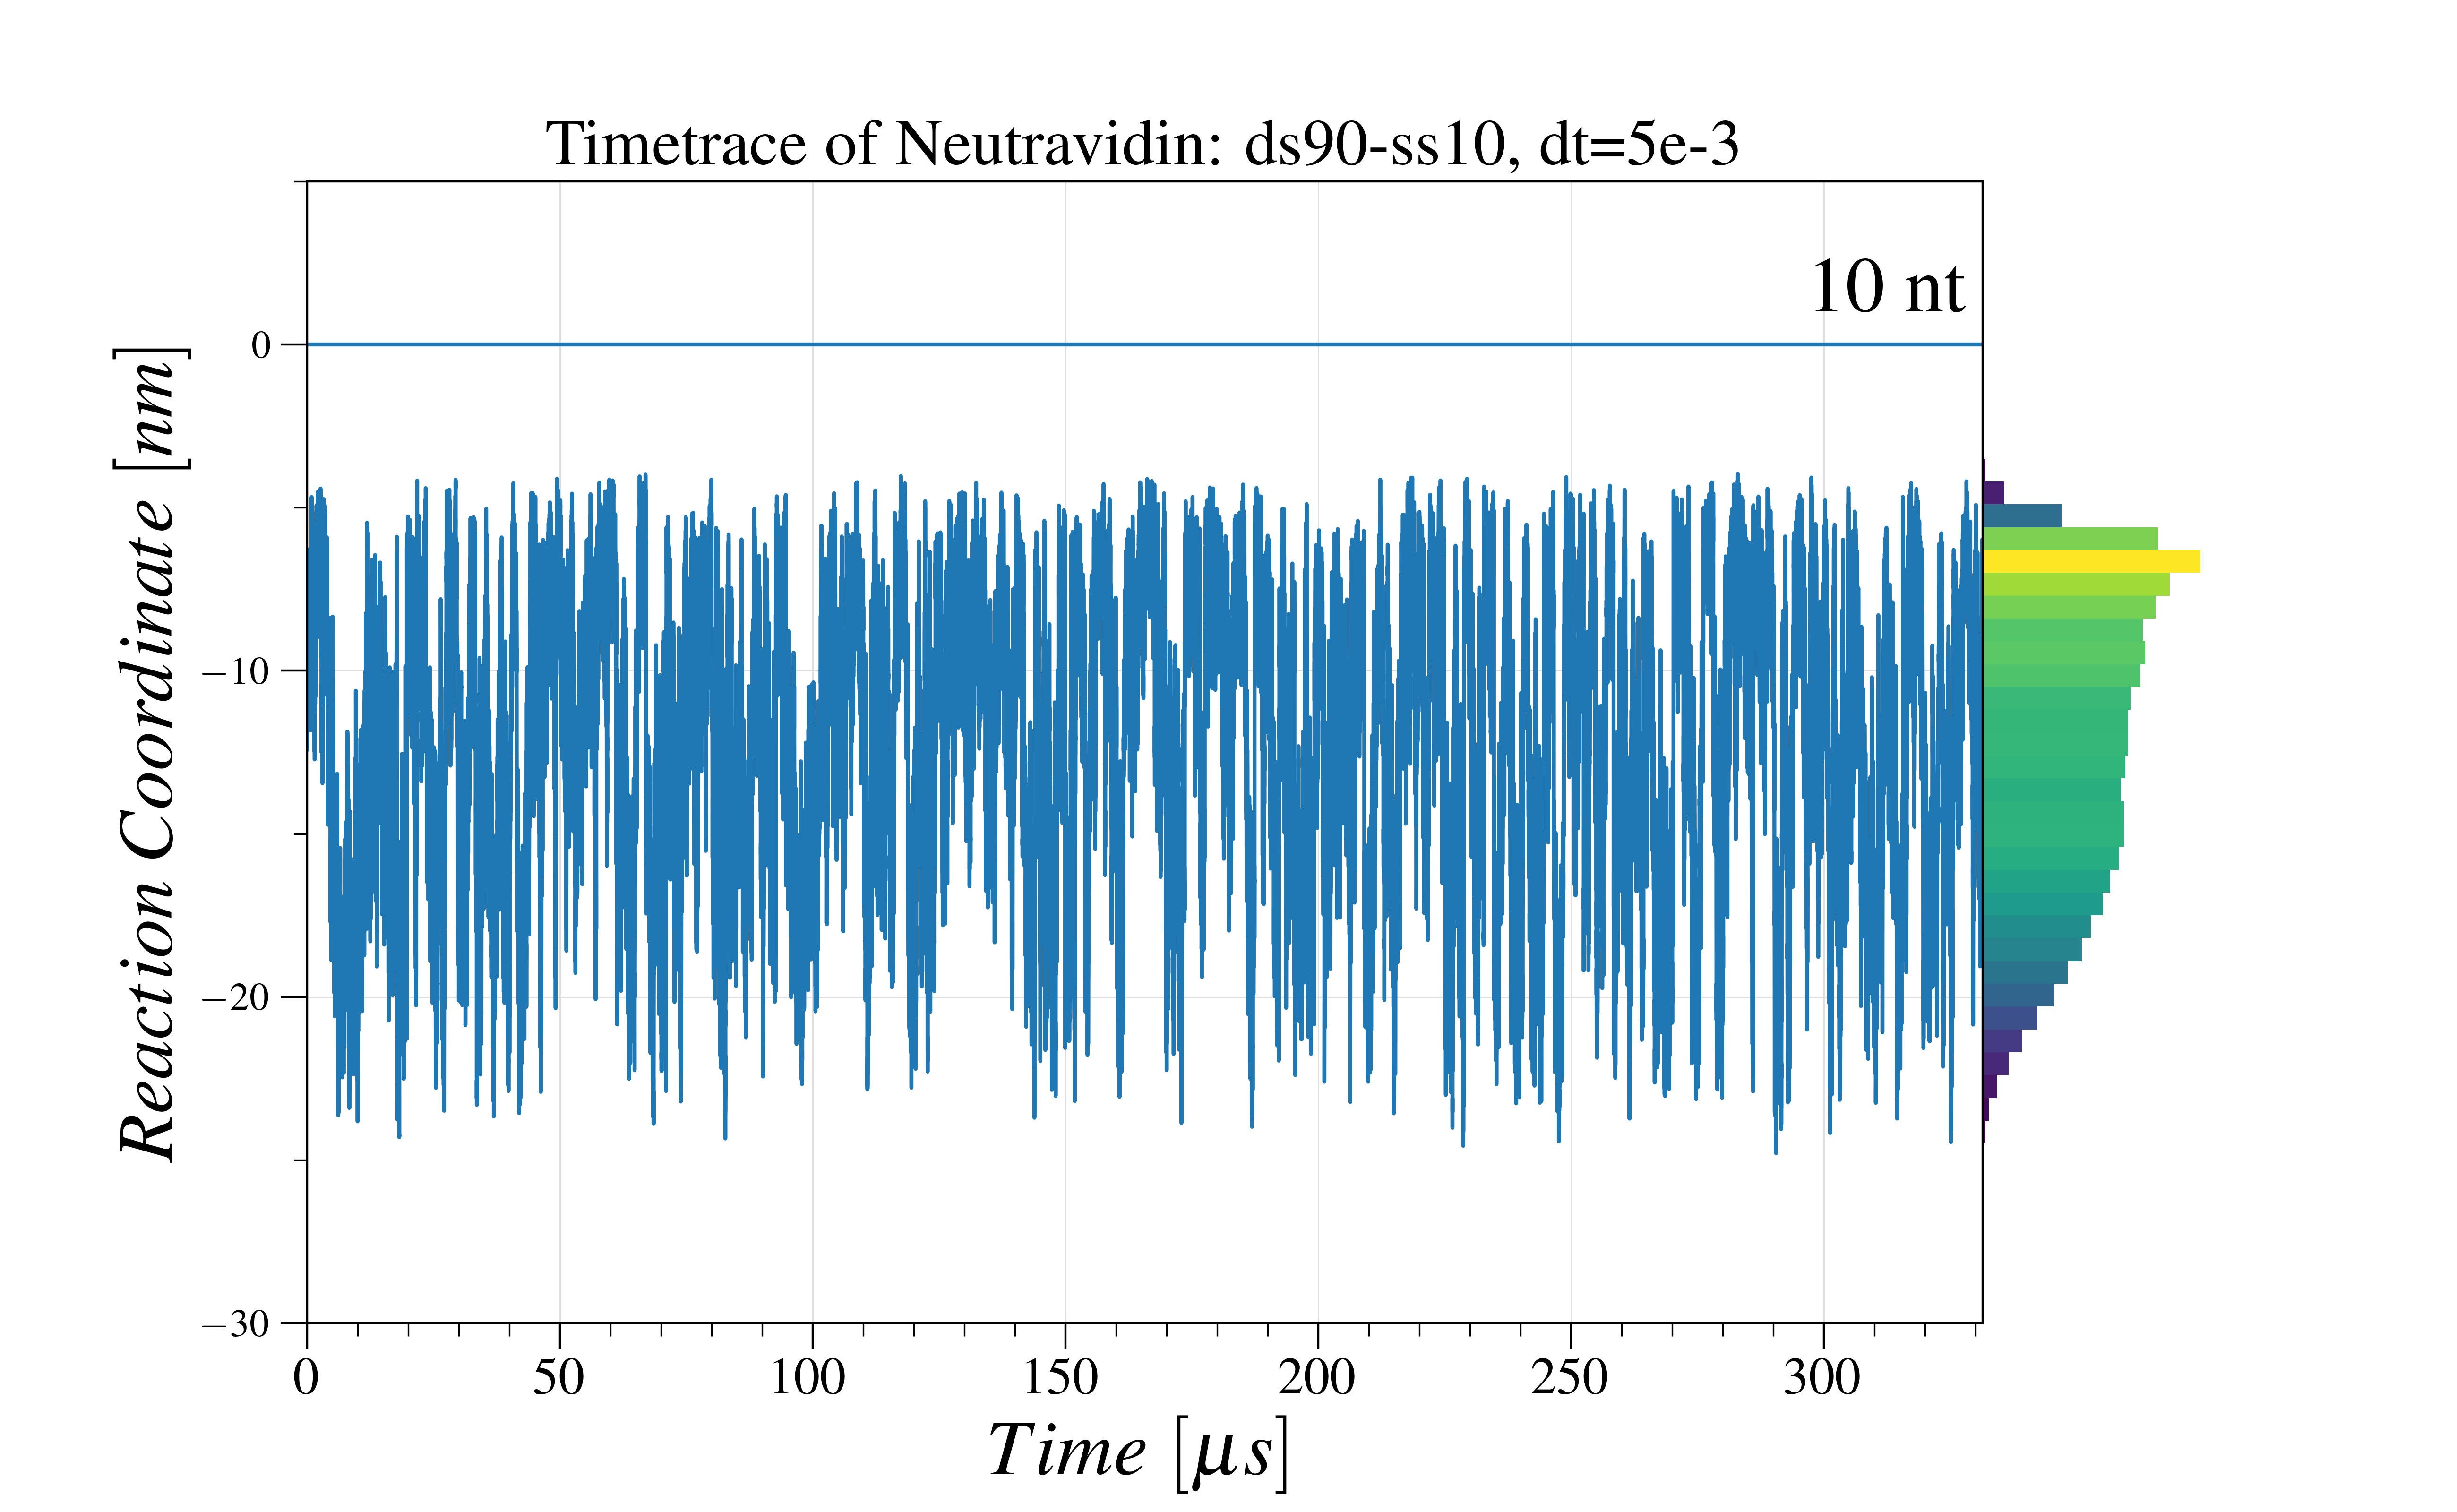
\includegraphics[width=.95\linewidth,valign=t]{Figures/MR-90.png}
  \end{subfigure}%
  \adjustbox{minipage=1.3em,valign=t}{}%
  \hspace{.3cm}
  \begin{subfigure}[t]{\dimexpr.21\linewidth-1.3em\relax}
  \centering
  \vspace{-0.5cm}
  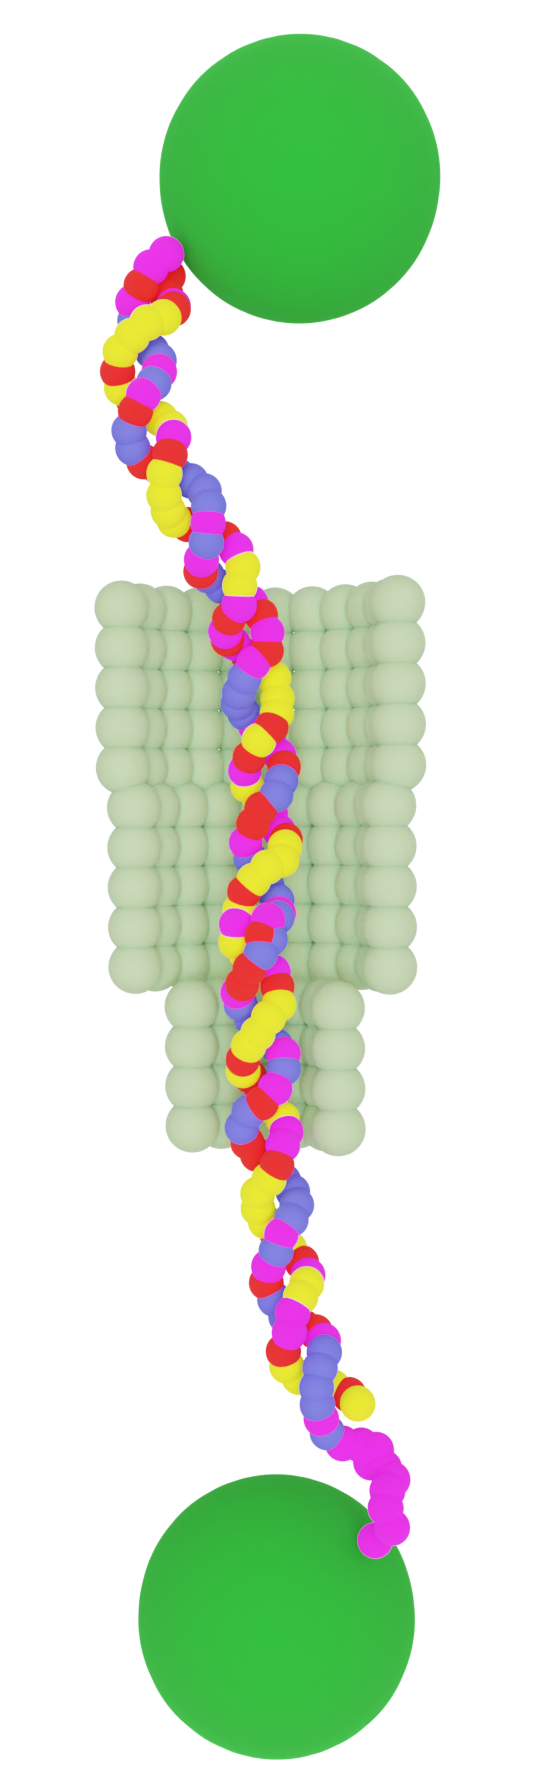
\includegraphics[width=.4\linewidth,valign=t]{Figures/Rotaxane-90.png}
  \end{subfigure}
  \label{fig:test}
  \end{centering}

  \vspace{.4cm}

  \begin{centering}
  \adjustbox{minipage=1.3em,valign=t}{}%
  \begin{subfigure}[t]{\dimexpr.3\linewidth-1.3em\relax}
  \centering
  \vspace{0.15cm}
  \hbox{\hspace{0.35cm}
  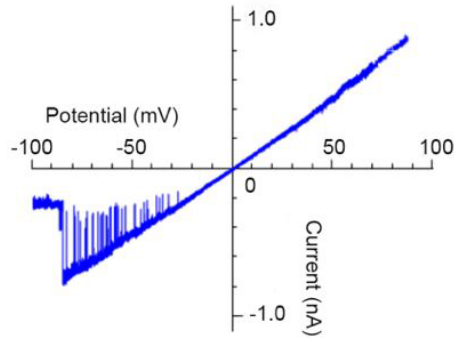
\includegraphics[width=1.05\linewidth,valign=t]{Figures/IV-80.png}}
  \end{subfigure}%
  \adjustbox{minipage=1.3em,valign=t}{}%
  \hspace{-0.5cm}
  \begin{subfigure}[t]{\dimexpr.5\linewidth-1.3em\relax}
  \centering
  \hbox{\hspace{0.56cm}
  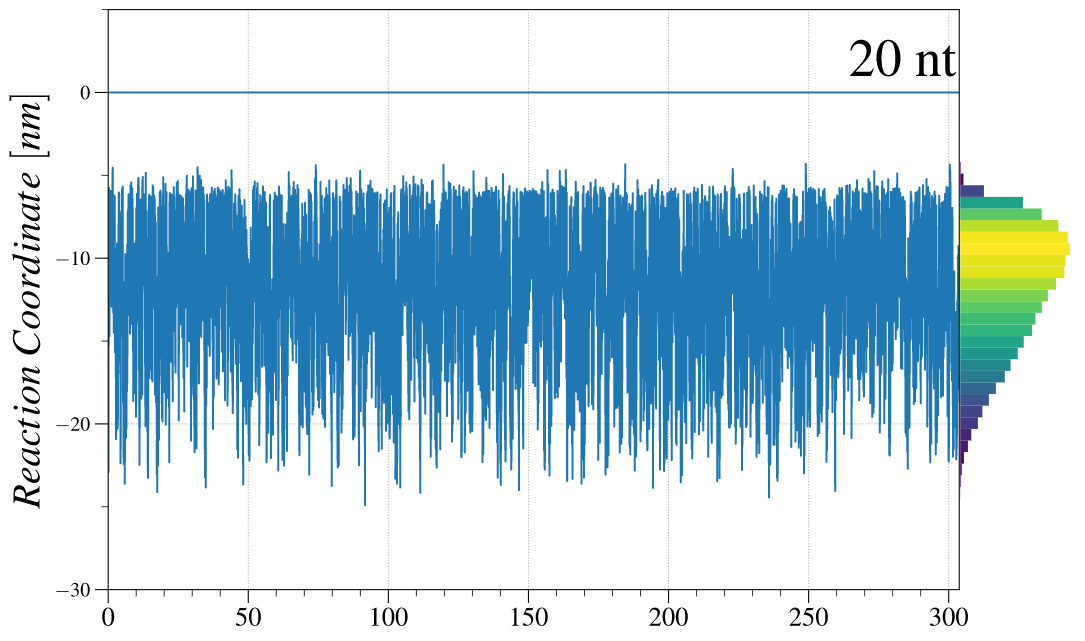
\includegraphics[width=.95\linewidth,valign=t]{Figures/MR-80.png}}
  \end{subfigure}%
  \adjustbox{minipage=1.3em,valign=t}{}%
  \hspace{.5cm}
  \begin{subfigure}[t]{\dimexpr.21\linewidth-1.3em\relax}
  \centering
  \vspace{-0.5cm}
  \hspace{-0.4cm}
  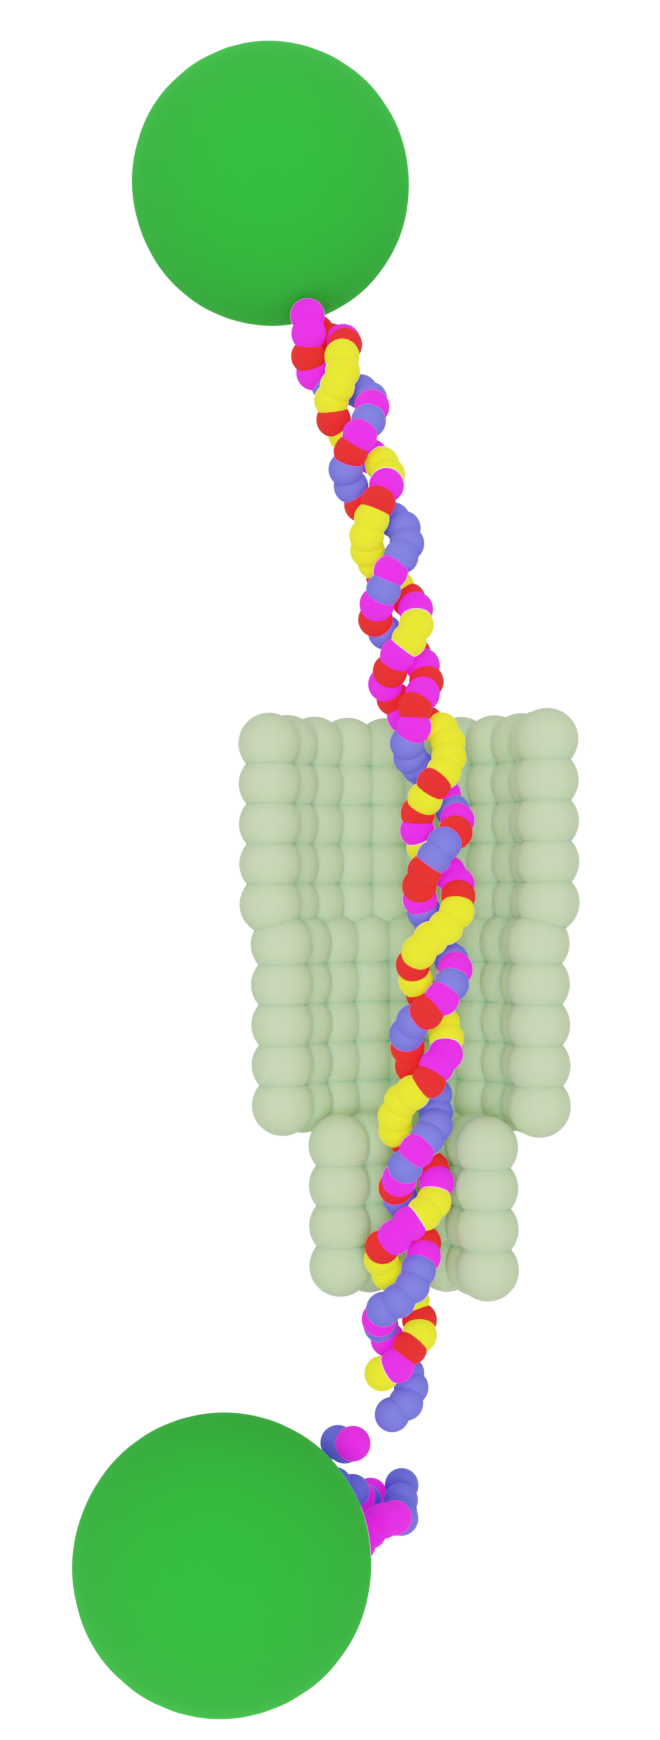
\includegraphics[width=.5\linewidth,valign=t]{Figures/Rotaxane-80.png}
  \end{subfigure}
  \label{fig:test}
  \end{centering}

  \vspace{.25cm}

  \begin{centering}
  \adjustbox{minipage=1.3em,valign=t}{}%
  \begin{subfigure}[t]{\dimexpr.3\linewidth-1.3em\relax}
  \centering
  \vspace{0.2cm}
  \hbox{\hspace{0.4cm}
  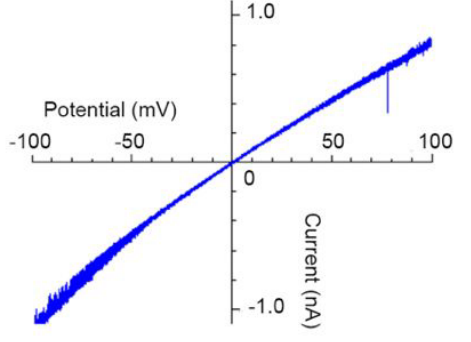
\includegraphics[width=1.05\linewidth,valign=t]{Figures/IV-70.png}}
  \end{subfigure}%
  \adjustbox{minipage=1.3em,valign=t}{}%
  \begin{subfigure}[t]{\dimexpr.5\linewidth-1.3em\relax}
  \centering
  \hbox{\hspace{0.15cm}
  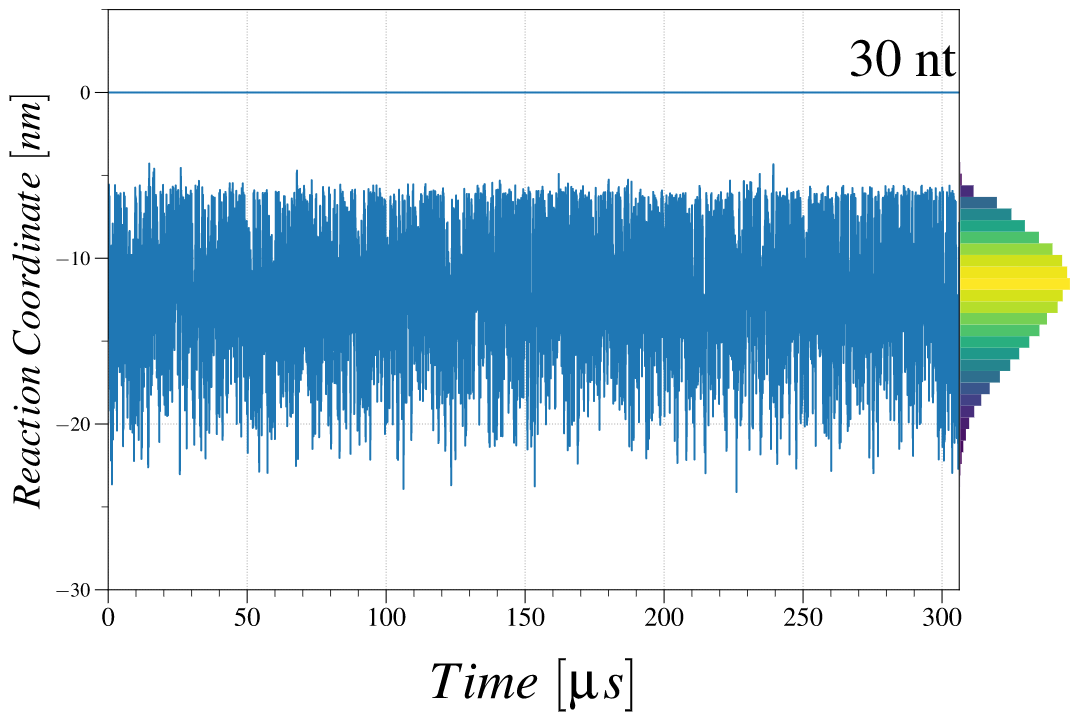
\includegraphics[width=.95\linewidth,valign=t]{Figures/MR-70.png}}
  \end{subfigure}%
  \adjustbox{minipage=1.3em,valign=t}{}%
  \hspace{0.5cm}
  \begin{subfigure}[t]{\dimexpr.21\linewidth-1.3em\relax}
  \centering
  \vspace{-0.6cm}
  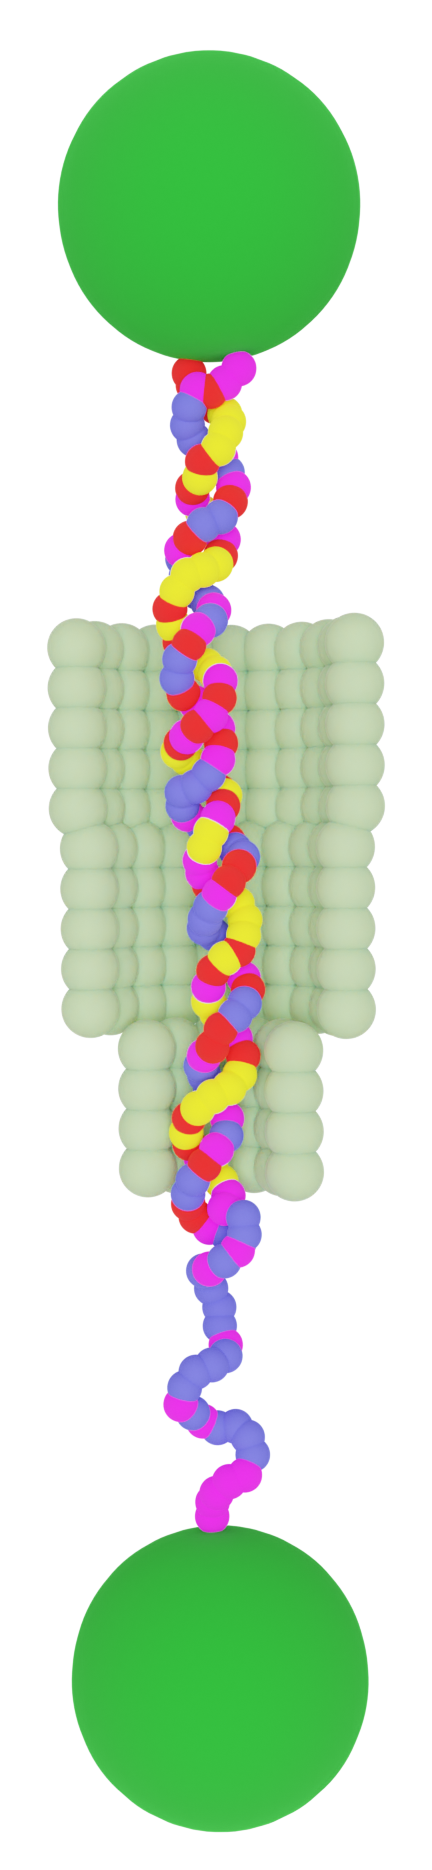
\includegraphics[width=.35\linewidth,valign=t]{Figures/Rotaxane-70.png}
  \end{subfigure}
  \label{fig:test}
  \end{centering}
  \caption[short lof/lot caption]{This is a figure.\vspace{2cm}}

\end{figure}

To interpret the observed characteristics in the I-V traces, molecular dynamics
simulation where performed of the mixed rotaxanes. The rotaxanes where simulated with no
bias, i.e. $0 mV$, to solely highlight the changes in the entropic effects. Quantifying
the conformational fluctuations of the rotaxane is done by tracing the trans-stopper
protein during the simulation using a reaction coordinate defined in our system. This
reaction coordinate, $X$, is determined as,
\begin{equation}
  X = \begin{cases}
        &z_0 + |\textbf{r} - \textbf{r}_{cis}|, \hspace{0.5cm} \textit{if on cis-side}\\
        &z, \hspace{2.5cm} \textit{if inside pore}\\
        &-|\textbf{r}|, \hspace{2.11cm} \textit{if on trans-side}
      \end{cases}
\end{equation}
Here the z-axis is aligned with the symmetry axis of the nanopore, placing the origin of
the coordinate system at center of the pore's trans-entrance. With respect to this
coordinate system, the center of pore's cis-entrance is located at $r_{cis} = (0,0,z_0)$.

In Figure ... the measured time trace of the $X$-coordinate is presented for each mixed
rotaxane type.  The horizontal line indicates the origin of the reaction coordinate,
representing the trans-entrance of the pore. On the right side of these graphs the $X$
histograms of the time traces are presented, indicating the positional distribution of
the trans-stopper during the simulations. It should be noted that the time traces are not
obtained from one continuous simulation, but rather aggregated from various independent
simulations performed in parallel, aiming to reduce the simulation time.

For the rotaxane fully composed of dsDNA, i.e. $0nt$, a uniform  $X$  histogram is found.
This result indicates free diffusion of the rotaxane within a bounded one dimensional
domain, namely the nanopore. In the case where $10nt$ and $20nt$ are substituted into the
composition of the rotaxane a peak is observed in the $X$ histogram. This peak indicates
a tendency of the trans-stopper to move towards the entrance of the nanopore. This
observation is in agreement with the previously discussed I-V curves, since the presence
of the stopper at the pore entrance partially blocks the current flow. This tendency
is driven by an entropic force arising from the smaller ssDNA strand, being more easily
captured in the constriction of the pore compared to the large dsDNA strand.


Next, we observe that increasing the length of the ssDNA part of the mixed rotaxane
gradually shifts the histogram's peak further away from the pore entrance. Confining a
portion of the freely fluctuating ssDNA strand inside of the pore,
drastically reduces the number of available configurational microstates and thereby also
its entropy. This change in entropy induces an opposing entropic force.
An equilibrium configuration is found, when both the large dsDNA is kept outside of the
constriction, while allowing a maximal length of ssDNA strand to freely fluctuate outside
of the pore. These combined effects shift the peak of the distribution further away from
the pore entrance as the number of nucleotides is increased. An ever larger
electrophoretic force is required to sustain full pore blockage, which is why no blockage
is observed in the experiment's voltage range. The results found in these simulations are
in accordance with the corresponding simulations performed by Bayoumi et al.[.], using
the bead-and-spring model.

As the final part in our analysis of the mixed rotaxanes, the confined diffusion of the
$0nt$ mixed rotaxane is studied. The uniform distribution of the $X$ histogram suggests
that the rotaxane vertically fluctuates inside of the pore like a rigid rod. To study
this diffusive behaviour, the mean square displacements(MSD) of the
trans-stopper is determined within a range of time intervals.\footnote{reference
tidynamics by Pierre de Buyl} Calculating the MSD is done by utilising a rolling-window
analysis on the measured time trace. The MSD is an important quantity used to
characterise diffusive processes, since it allows us to verify whether an external force
influences the motion. From analytical calculations, presented in appendix A, we find
that one dimensional confined diffusion can be described up to the second order as,
\begin{equation*}
\langle \Delta x \rangle = \frac{L^2}{6} - \frac{96}{\pi^4} e^{-\frac{D \pi^2t
}{L^2}},
\end{equation*}
here $L$ is the length of the confined region, i.e. the hight of the pore, and $D$ the
diffusion constant of the particle. This model was fitted to our simulations, for which
the result is presented in Figure... From this we can conclude the $0nt$ mixed rotaxane
can be well described using the simple model of one dimensional confined diffusion,
confirming our postulation. This model predicts the diffusion coefficient of the mixed
rotaxane as, $69.08 \pm 0.02 \mu s^{-1}$, giving us an idea of the speed of the
rotaxane dynamics.

\begin{figure}[ht!]
\begin{center}
  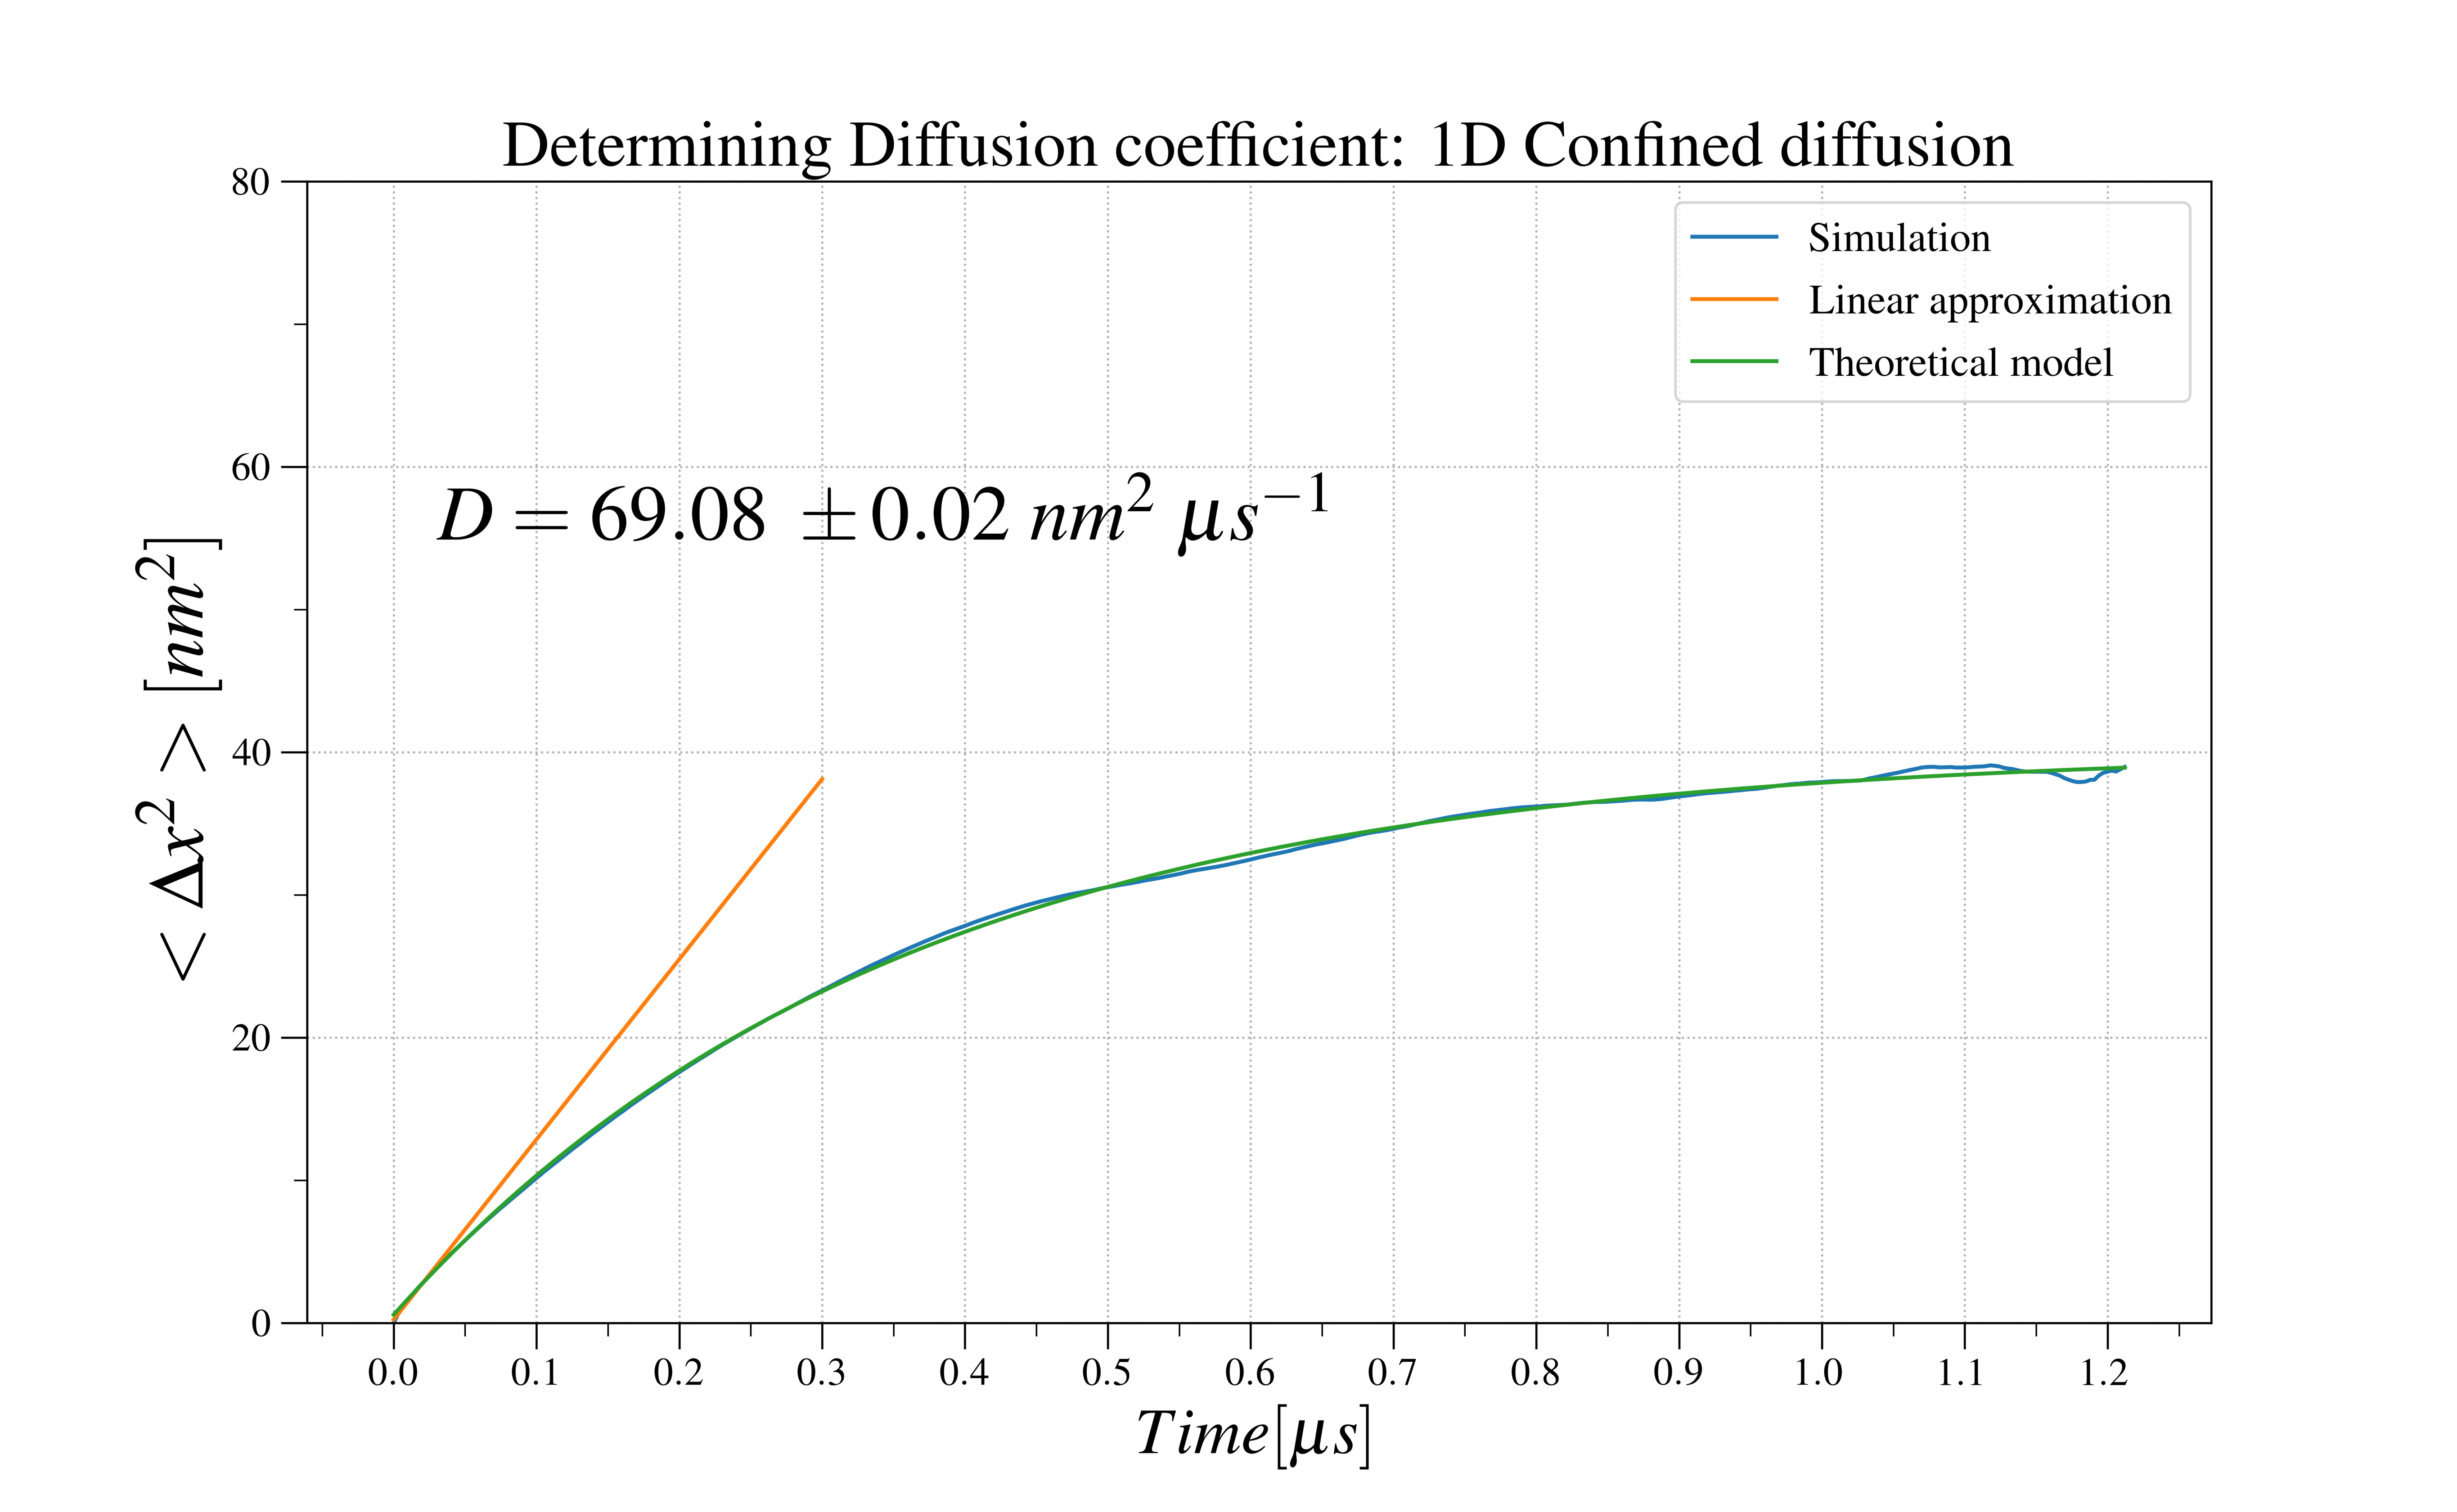
\includegraphics[width=\textwidth]{Figures/MR-100-diff.png}
  \caption[short lof/lot caption]{write caption}
\end{center}
\end{figure}

\section{Conformational Fluctuations of the ds- and ss-Rotaxanes}

Having gained insight into the entropic interactions between the DNA and the
nanopore in the mixed rotaxanes, now the stable intermediate states of the nanopiston's
operation cycle are
studied. Both the rotaxane-ss and -ds are composed of stiff dsDNA and flexible ssDNA
parts, which characterise their conformational fluctuations by the entropic interactions.
The two rotaxanes types are simulated in a nanopore, using the predefined coarse-grained
model, in absence of an external bias, i.e.  $0mV$. The results are presented in Figure
\ref{fig:conform}

Analysing the conformational fluctuations of the rotaxane-ds, we observe from the blue
histogram that the ssDNA
overhang remains predominantly outside of the pore. This effect can be explained by
taking
into account the entropic cost of capturing the flexible strand of ssDNA into the
constriction of the pore. Since the geometry of the rotaxane prohibits the overhang from
reaching the cis-side of the pore, the overhang can only freely fluctuate on the
trans-side of the pore. Throughout the simulation this entropic force keeps the overhang
in the trans-reservoir and thereby placing the cis-protein stopper close to the entrance
of the pore. This entropic interaction plays an important role in the operation of the
nanopiston. Even when an external voltage difference induces an upward electrophoretic
force on the rotaxane, the competing entropic force keeps the overhang outside of the
constriction and thereby exposing it for hybridisation with a fuel strand. This also
explains the halting of the piston cycle at high voltages. In this case the entropic
force is overcome by the induced electrophoretic force, sequestering the overhang inside
of the pore inhibiting the binding of fuel strands.

In the same figure the results for the rotaxane-ss are presented. We observe that the
histograms are shifted upwards, indicating an upwards entropic arising from the high
flexibility of the long ssDNA strand. This force originates from the increase in
configurational microstates available to the rotaxane-ss, when the ssDNA strand is
allowed to freely fluctuate in the
cis-reservoir. The flexibility of the ssDNA strand overcomes the entropic penalty of
confining the dsDNA into the constriction of the pore. Capturing the interface between
the ssDNA and dsDNA parts of the rotaxane-ss inside of the pore promotes the
operation cycle. In this case a longer ssDNA strand is exposed to the cis-reservoir,
better facilitating the hybridisation with cargo strands. This can be seen in the
positional histogram of the cis-protein stopper, where the large fluctuations of the
ssDNA strand allow it to venture far away from the nanopore.

These results explain the functional importance of the entropic interactions in the
nanopiston's operating cycle. Comparing our findings with the simulation results by
Bayoumi et al., we see that both models are in reasonable accordance. However, in our
simulations the interface of the rotaxane-ss is observed entering inside the pore's
constriction, while in the bead-and-spring model this behaviour is not observed. This
difference can be attributed to the more accurate simulating of ssDNA by OxDNA, mainly
arising from the more precise parametrisation of the model and the ability for
consecutive bases to unstack.

\begin{figure}[ht!]
\begin{center}
  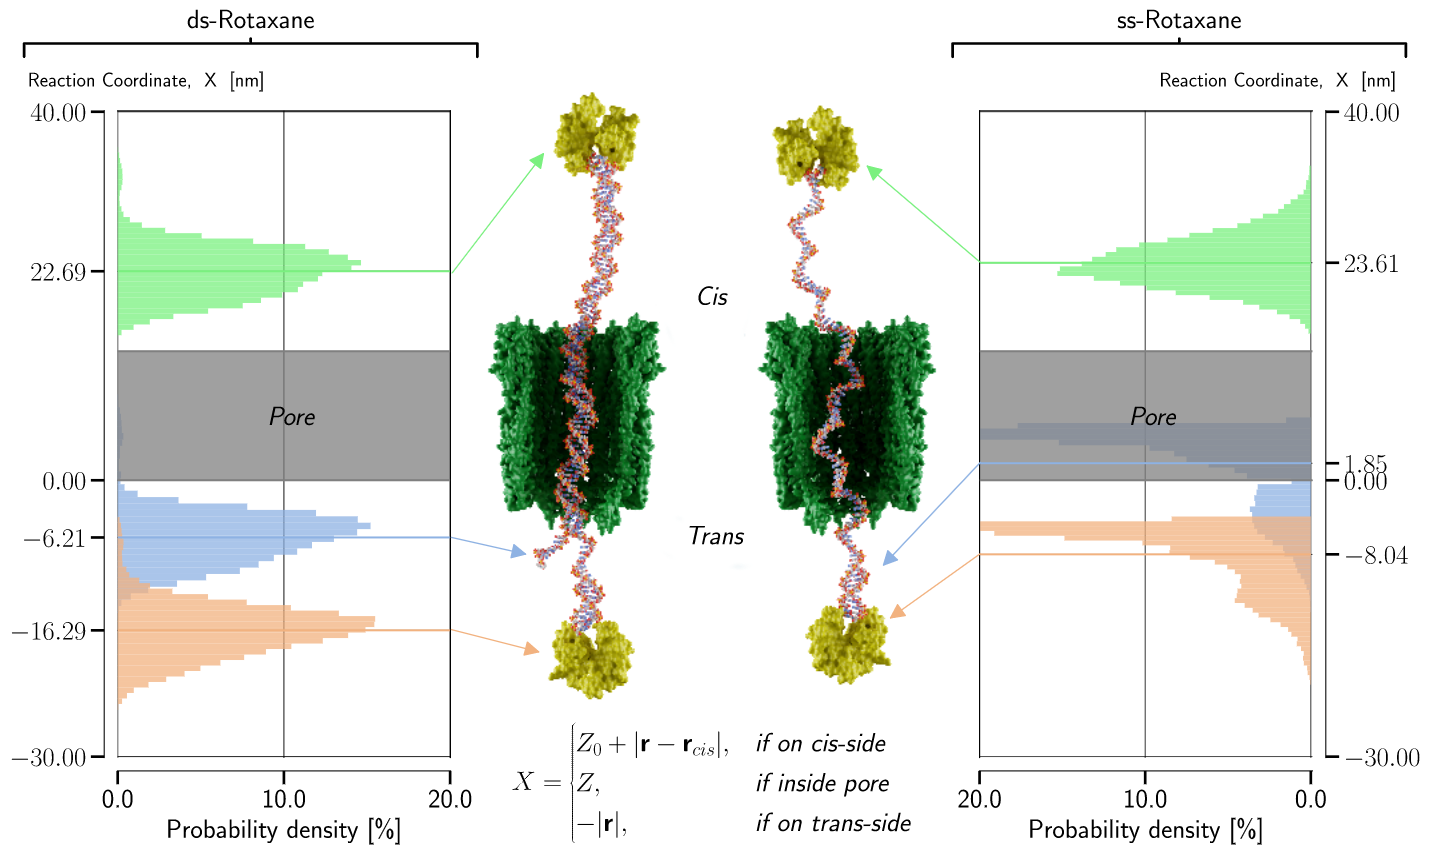
\includegraphics[width=1\textwidth]{Figures/image.png}
   \caption[Conformational fluctuations of the ss- and
ds-rotaxane.]{\linespread{0.5}{\small Conformational fluctuations of the rotaxane-ds
    (left) and -ss (right). In the center renders of the atomistic structure for both
    rotaxane variants are shown. On the sides the $X$-histograms, see definition, for
    selected components of the rotaxanes are presented. The mean values of the
    $X$-coordinates are marked by the horizontal lines. From the results we conclude that
    the flexible ssDNA strands determine the fluctuations of the rotaxanes-ds and -ss.
    Central images were rendered using Blender.\cite{blender}}}
\label{fig:conform}
\end{center}
\end{figure}

\section{Hybridisation Reactions in the Piston Cycle}

Hybridisation reactions are central to the operation cycle of the DNA nanopiston. By
providing the required free energy, they facilitate the transitions between the two
stable states of the cycle, rotaxane-ss and rotaxane-ds. Combining these transitions with
the previously discussed entropic interactions leads to a ratcheting mechanism, enabling
the extraction of useful work from the intrinsicly stochastic system.

% The associated length and time scales of these reactions make their in-depth analysis
% experimentally challenging. For this reason scientists resort to computational
% simulations for high resolution analyses of these reactions.
To study the DNA
hybridisation occurring during the piston operation cycle, we utilise our OxDNA based
model of the piston, which is simulated using molecular dynamics. As previously discussed
in chapter three, the intrinsic energy landscape associated with these reactions
complicates brute force simulations of the transitions. To overcome these limitations a
forward flux sampling algorithm is employed. The order parameter used in these
simulations is based on the number of correclty hybridised basepairs. The phase space is
thus partitioned with $80$ hypersurfaces, where the interface of $\lambda_i$ corresponds
to $i$  formed basepairs in the hybridisation reactions. Generating the transition
pathways between these interface is done using the Rosenbluth-like (RB) method, described
in Chapter 3.3.

To illustrate the viability of this
technique, first both the hybridisation and strand displacement reactions of the
rotaxanes are simulated outside of the nanopore. From these simulations it is
confirmed that using the forward flux sampling algorithm the full ensemble of transition
pathways, present in the hybridisation reactions, can be studied.

However, performing these same simulations with the rotaxanes placed inside of the
nanopore inhibits the reaction from occurring. Initially the simulations for both the
strand displacement and hybridisation reaction show comparable behavior to the
simulations performed outside of the pore. However, during the final stages of these
simulations the geometry of the rotaxane forces three ssDNA strands inside of the pore's
constriction. The diameter of the pore was modelled to carefully capture both the
electrostatic and excluded volume interactions between the ClyA pore and the DNA.
This results in a diameter of $2.9\ mm$, compared to the $1\ nm$ width of the ssDNA
strand.
Due to the static nature of our coarse-grained pore model, the diameter of the pore
constriction does not facilitate the three ssDNA strands to enter the constriction
simultaneously.

Molecular dynamics simulations performed by Willems et al.\cite{Willems2020} indicate
that the $\alpha$-helices constituting the pore's constriction allow for structural
fluctuations of the constriction. The per-residue b-factor of ClyA-AS was used to study
the flexibility of the side-chains in the protein complex. The calculated b-factor is
proportional to the mean square displacement of a specific residue\footnote{Refers to a
single amino acid
monomer in the protein.} in the ClyA-AS, averaged over all
$12$ monomers in the protein complex. Here, we observe that the residues corresponding to
the $\alpha$-helices in the constriction are found to have a large b-factor and thus
fluctuate significantly.

Our simulations indicate that the compliancy of the pore
entrance is essential in the hybridisation reactions of the rotaxanes. However, during
the design of our coarse-grained model this compliancy was not taking into account. This
limitation of our coarse-grained model impedes the full analysis of the DNA nanopiston's
operating cycle.

To resolve this limitation of our model, an attempt was made to incorporate these
fluctuations in the simulations. This was done by allowing the constituent beads of the
nanopore constriction to fluctuate during the simulation. To stabilise the protein
structure FENE bonds were used to connect the beads and retain the cyclindrical structure
of the pore. Parameterising these interatomic bonds was found to be challenging and was
not successful within the time constraints of this thesis.

% \begin{figure}[ht!]
%   \centering
%   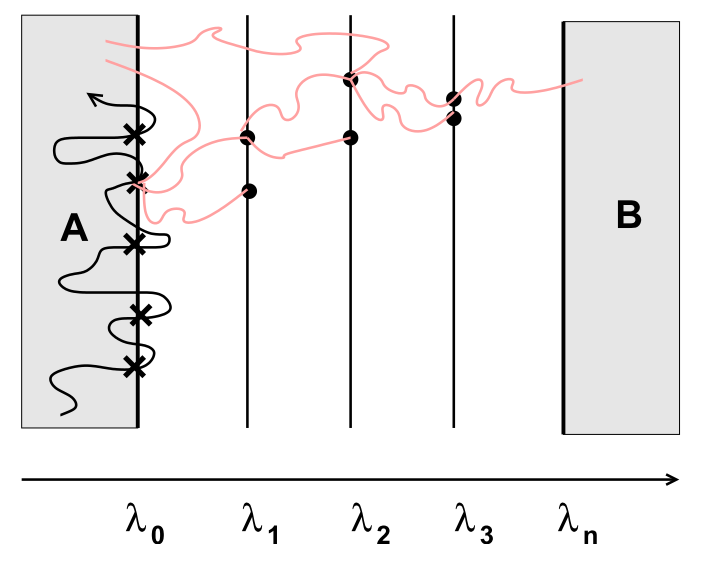
\includegraphics[width=0.6\linewidth]{Figures/FFS.jpg}
%   \caption{Nog maken}
% \end{figure}



\chapter{Conclusions and Perspectives}
\vspace{-1cm}
\epigraph{All models are wrong, but some are useful.}
{--- \textup{George Box}}
\noindent In this work the novel molecular machine devised by Bayoumi et al. has been
studied using
molecular dynamics simulations. The primary objective of this research was to shed
light on the operating principles facilitating the autonomous and active transport which
characterise this DNA nanopiston. In this chapter the obtained results are summarized,
after which recommendations for future research are made.

\section{Results \& Conclusions}

Understanding the underlying processes driving the operation of molecular machines is an
important corner stone in furthering their development. As a result of the scale and
complexity of these structures, shedding light on these interactions is experimentally
challenging. In this work we aimed to provide an insight into the operation of the
DNA nanopiston using molecular dynamics simulations.

This thesis builds further upon simulations presented in the original paper, where a
coarse-grained model of the DNA nanopiston was developed based on both theoretical and
experimental considerations. The central component of this model is the DNA rotaxane
which was simulated using a bead-and-spring model. To increase the scope of the research,
we designed a new coarse-grained model of the DNA nanopiston utilising a more accurate
representation of DNA, namely OxDNA. This new model yields a more realistic description
of DNA while also enabling us to simulate DNA hybridisation reactions.

The entropic penalty of confining single stranded DNA inside of the nanopore is presumed
to play an important role in the mechanisms driving the DNA piston. We studied these
entropic effects by simulating a specifically engineered class of rotaxanes, called the
mixed rotaxanes. These simulations indicate that there are two competing entropic
interactions present in the rotaxane-pore complex. A first entropic force is found to
arise from confining the large dsDNA strands of the rotaxane inside of the pore.
Competing with this force are the smaller but more flexible ssDNA strands which endeavour
to maximize their available configurational space by opposing the confinement of the
pore. As the length of these ssDNA strands is increased, this latter interaction starts
to dominate.

After establishing this essential understanding of the entropic interactions, the two
stable states of the piston's operating cycle are simulated, i.e. rotaxane-ss and
rotaxane-ds. These simulations indicated that the sequestering of the overhang of
rotaxane-ss is prevented by the entropic penalty of confining it in the pore.
The established entropic force enables the hybridisation with fuel strands even opposing
an upward electrophoric force, differentiating the DNA nanopiston as an active
transporter. Due to the rotaxane geometry this hybridisation reaction results in the
formation of rotaxane-ss in a low-entropy state. As a consequence the rotaxane-ss
spontaneously migrates in the trans-cis direction exposing the flexible ssDNA strand to
the cis-reservoir, enclosing the dsDNA fraction inside of the pore. This
upward motion plays an important role in exposing the ssDNA fraction of rotaxane-ss to
the cis-reservoir, where it can hybridise with a cargo strand. Here we concluded that
the interplay of the hybridisation reactions and the entropic interactions collectively
drive the molecular machine.

In the last part of this thesis an attempt was made to study the ensemble of
hybridisation pathways providing the free energy to drive the nanopiston. The study of
these thermodynamic transitions was complicated by the complex reaction kinetics and an
initial energy barrier. To overcome this difficulty an forward flux sampling algorithm
was used to analyse these transitions. From the performed simulations we concluded that
the static representation of the ClyA pore in our coarse-grained model inhibits these
hybridisation reactions. The compliance of the pore constriction is found to be essential
in facilitating the hybridisation reactions, yet were not incorporated in our model.

The performed computational analysis of the DNA nanopiston confirmed earlier research on
the operating principles facilitating the piston cycle. The exploratory research that was
performed motivates further exploration towards the functioning of this nanopiston.
This exploratory research motivates further research around the operation of this
molecular machine. Eventually, this knowledge will aid the development of novel molecular
devices, further blurring the line between nature and the artificial.

\section{Future Perspectives}

During this thesis we were able to deepen our understanding of the DNA
nanopiston. However, some important questions remained unanswered. While studying the
hybridisation reactions, which drive the molecular machine, we encountered the
limitations of
our coarse-grained model. Simulations indicated that the compliancy of the nanopore
is an essential component in facilitating these reactions. In our current model the ClyA
nanopore is represented as a static complex, not allowing the diameter fluctuations that
are needed for the hybridisation to take place.
Future research should attempt to incorporate a more accurate representation of the ClyA
nanopore in the coarse-grained model of the DNA nanopiston.

Various approaches can be taken to accomplish this improved accuracy.
A first proposition would be to expand further upon the existing model, by
incorporating the constriction of the pore in the Langevin integrator. Using experimental
data, we can parameterise the interactions between the constituent beads of the pore and
reproduce the diameter fluctuations of the constriction of ClyA. Another
possible solution could be to use an already parameterised coarse-grained model.
An example of such a model is the Martini force-field, which allows for accurate
simulations of
transmembrane proteins, like the ClyA pore. In this new model both OxDNA or the Martini
force-field could be integrated to simulate the DNA strand. These suggested improvements
would increase the accuracy of our model, probably enabling the simulation of a full
piston cycle.

Molecular dynamics simulations will proof to be a useful tool in the development of
new molecular machines. Future research is focused on designing molecular devices that
are able to not only transport DNA, but also other molecules through a membrane.
Eventually, the aim would be to implement these new molecular machines into a
sophisticated droplet-based device with emergent properties, i.e. a fully synthetic cell.




% APPENDIX
\begin{appendices}
\addtocontents{toc}{\protect\setcounter{tocdepth}{1}}
\chapter{One Dimensional Confined Diffusion}

This appendix provides a detailed description of the motion of a Brownian particle
confined to a one dimensional domain. Due to the stochastic nature of this motion, we
will discuss the evolution of the probability density function $\phi(x,t)$, which
represents the probability of finding the particle on the position $x$ at time t.
Once the evolution of this probability function is known, the statistical properties can
be evaluated. Here, we will discuss the Mean Square Displacement (MSD), as it is used to
analyse the motion of the $0nt$ mixed rotaxane.\\
A central result in statistical mechanics is that the evolution of
$\phi$ is  described by the diffusion equation, given by
\begin{equation}
  \frac{\partial \psi}{\partial t} =  D \frac{\partial^2 \psi}{\partial x^2}, \quad
  \label{eq:diff}
\end{equation}
where D is the diffusion coefficient of our particle.
The confinement is imposed through reflecting boundary conditions at $x=0$ and $x=L$,
which is equivalent to imposing a
vanishing particle current at the boundaries of our domain, $j = - D \frac{\partial
\psi}{\partial x} = 0$. Solving equation \ref{eq:diff} can be done using the
method of
separation of variables, where we assume that the solution can be expressed as $
\psi(x,t) = f(x)g(t)$. Upon this substitution Eq. \ref{eq:diff} becomes,
\begin{equation}
  \frac{\dot{g}}{g} = \frac{\ddot{f}}{f} = - \alpha,
\end{equation}
where the two expressions are implied to be constant since the variables are independent.
The partial differential equation is now treated as two seperate ordinary differential
equations, for which we find,

\begin{align}
t:\quad \dot{g} = - \alpha g(t) \Rightarrow g(t) = e^{-\alpha t},
\end{align}

\begin{align}
  x:\quad D \ddot{f} = - \alpha f(x) \Rightarrow f(x) &= A \sin(K x) + B \cos(Kx)\\
  &= B \cos(\frac{\pi n x}{L}).
\end{align}
In the latter expression the boundary conditions impose that $A=0$ and constrain the
parameters by the relation,
\begin{align}
  \frac{\alpha}{D} = \frac{\pi^2 n^2}{L^2}.
\end{align}
By substituting the found results into the assumed form of the solution, we find the
general solution to the confined diffusion equation as the linear combination,
\begin{align}
  \psi(x,t) &= \sum_{n=0}^{+\infty} C_n \cos\Big(\frac{\pi n x}{L}\Big) e^{- \frac{D\pi^2
  n^2}{L^2}t}.
\end{align}
At time $t=0$ the particle is assumed to be found at $x_0$ resulting in the initial
condition,
\begin{align}
  \psi(x, 0) = \delta(x-x_0) = \sum_{n=0}^{+ \infty} C_n \cos(\frac{\pi n x}{L}).
\end{align}
Imposing this initial condition on the found general solution of the confined diffusion
equation gives,
\begin{align}
  \psi(x, t)=\frac{1}{L} \Bigg[ 1 + \sum_{n=1}^{+\infty} \cos\Big(\frac{\pi n
  x_0}{L}\Big) \cos\Big(\frac{\pi n x}{L}\Big) e^{- \frac{D\pi^2  n^2}{L^2}t}\Bigg].
\end{align}
This expression describes the behaviour of a Brownian particle in a one dimensional
confined domain. Using the found expression the MSD is calculated to be,
\begin{align}
  \langle \Delta x^2 \rangle &= \langle(x-x_0)^2\rangle\\&= \frac{L^2}{6}\Bigg[1 -
  \frac{96}{\pi^4}
  \sum_{k=0}^{+\infty} \frac{1}{(2k+1)^4} e^{- \frac{D(2k+1)^2 \pi^2}{L^2}t}\Bigg].
\end{align}
As expected, the mean square distances saturates to $\langle \Delta x^2 \rangle = L^2/6$
in the long-time limit $t \gg L^2 / D.$ To explore the other limiting case $t \ll L^2/D
$, we perform a Taylor expansion of the exponential and find,
\begin{align}
  \langle \Delta x^2 \rangle &= \frac{L^2}{6} - \frac{16 L^2}{\pi^4} \sum_{k=0}^{\infty}
  \frac{1}{(2k+1)^4} + \frac{16 D t}{\pi^2} \sum_{k=0}^{\infty} \frac{1}{(2k+1)^2} +
  \mathcal{O}\bigg(\frac{D^2 t^2}{L^4}\bigg).
\end{align}
Using the two convergent series,
\begin{equation}
  \sum_{k=0}^{\infty} \frac{1}{(2k+1)^2} = \frac{\pi^2}{8} \qquad \text{and} \qquad
  \sum_{k=0}^{\infty} \frac{1}{(2k+1)^4} = \frac{\pi^4}{96}
\end{equation}
the free diffusion is recovered at short time scales,\cite{BICKEL200724}
\begin{equation}
  \langle \Delta x^2 \rangle = 2Dt \qquad \text{for }\,\, t \ll L^2/D.
\end{equation}

\end{appendices}

% BIBLIOGRAPHY
% \addcontentsline{toc}{chapter}{Bibliography}
% \begin{multicols}{1}
% \begin{smallfont}
\twocolumn
% \bibliography{Bibliography/thesis.bib}
\printbibliography
% \end{smallfont}
% \end{multicols}
% \cleardoublepage

\onecolumn
% \thispagestyle{empty}
\chapter*{Acknowledgements}
\addcontentsline{toc}{chapter}{Acknowledgements}
...

\cleardoublepage
\thispagestyle{empty}

% Back side of book
\cleartoleftpage{} % Make sure the back page is at an even page number


% ----------------------- Achterblad ------------------------------
% Vergeet niet de tekst aan te passen:
% - Afdeling
% - Adres van de afdeling
% - Telefoon en faxnummer
% -----------------------------------------------------------------
\thispagestyle{empty}
\sffamily
%
\begin{textblock}{191}(102,-22)
{\color{blueline}\rule{160pt}{5.5pt}}
\end{textblock}
%
\begin{textblock}{191}(157,-22)
{\color{blueline}\rule{5.5pt}{59pt}}
\end{textblock}
%
\begin{textblock}{183}(-35,-22)
\textblockcolour{}
\flushright
\fontsize{7}{7.5}\selectfont
\textbf{DEPARTEMENT NATUURKUNDE EN STERRENKUNDE}\\
Celestijnenlaan 200d bus 2412\\
3000 LEUVEN, BELGI\"{E}\\
tel. + 32 16 32 71 24\\
fys.kuleuven.be\\
\end{textblock}
%
\begin{textblock}{191}(145,-16)
\textblockcolour{}
\includegraphics*[height=16.5truemm]{Figures/sedes}
\end{textblock}
%
\begin{textblock}{191}(-31,224)
{\color{bluetitle}\rule{544pt}{55pt}}
\end{textblock}


\end{document}
